\documentclass[10pt]{article}
\usepackage{commands}

\begin{document}
\begin{tcolorbox}
  \begin{center}
  \begin{Large}
    \textbf{PHYS 353 (Advanced Statistical Mechanics) Notes} \\
    \vspace{5pt}
  \end{Large}
  \begin{large}
        Rio Weil \\
\vspace{5pt}
    \emph{This document was typeset on \today}
  \end{large}
  \end{center}
\end{tcolorbox}

\begin{center}
  \textbf{Introduction:}

  This is a set of lecture notes taken from UChicago's PHYS 353 (Advanced Statistical Mechanics), taught by Peter Littlewood. Topics covered include the discrete to continuous transition, the ferromagnetic and antiferromagnetic Heisenberg chain, Ginzburg-Landau Theory, Fluctuations, The Scaling Hypothesis, The Renormalization Group, Perturbative RG, Continuous Symmetries, the non-linear $\sigma$ model, the 2-D XY model, Disorder and random system, Random fields, Spin glasses, Replica symmetry breaking, Neural networks and Boltzmann machines, and Non-equilibrium dynamics.
  
\end{center}
\addtocontents{toc}{\protect\hypertarget{toc}{}}
\tableofcontents

\newpage
\section{Introduction}
\emph{I was 34 minutes late to lecture due to misunderstanding the start time - thanks to Kalpak for providing his notes!}

\subsection{Probabilities in Statistical Mechanics}
In stat mech, probabilities are given by:
\begin{equation}
    P(\mu) = \frac{e^{-\beta H(\mu)}}{Z}
\end{equation}
for a microstate $\mu$. Here, $Z$ is the partition function:
\begin{equation}
    Z = \sum_\mu e^{-\beta H(\mu)}
\end{equation}
and $\beta = \frac{1}{k_B T}$ is the inverse temperature. The free energy can be obtained as:
\begin{equation}
    F = -\frac{1}{\beta}\ln Z
\end{equation}

What is meant by a state $\mu$? In some sense, there is a tension, as one slices up the continuous state space of classical physics. This is resolved by fields.

\subsection{Spin Models}
A rich setting to explore statistical mechanics is spin models. For example, the celebrated \emph{Ising model}is defined by the Hamiltonian:
\begin{equation}
    H_{\text{Ising}} = \sum_{ij}J_{ij}S_iS_j
\end{equation}
with $J_{ij}$ the coupling between classical spins $S_i \in \set{1, -1}$. We can also generalize this for arbitrary spin directions by promoting the spins to vectors (giving rise to a continuous degree of freedom), yielding the Heisenberg model:
\begin{equation}
    H_{\text{Heisenberg}} = \sum_{ij}J_{ij}\v{S}_i \cdot \v{S}_j.
\end{equation}

As is clear from the sums appearing in the above expressions, we are considering discrete spins (perhaps on some lattice). We can convert to momentum space via a Fourier transform, and then via a ``coarse-graining procedure'' (formalized by the renormalization group) we obtain a roughly continuous spectrum, which we may treat as a field.

\subsection{From discrete models to fields}
For example, we can consider the linear dispersion relation:
\begin{equation}
    \omega(k) = c\abs{k}
\end{equation}
which gives rise to the density of states:
\begin{equation}
    d^3n = u(k)d^3k = u(\omega)d\omega
\end{equation}
Which by then considering a sphere in $k$-space of surface area $4\pi k^2$ this becomes:
\begin{equation}
    qu(\omega) = u(k)4\pi k^2 \frac{dk}{d\omega}
\end{equation}
The energy density $u(k)$ we take to be constant, i.e. just $V/(2\pi)^d = L^3/(2\pi)^d$ (for a box of length $L$) and $\dod{k}{\omega}$ is obtained from the dispersion relation, yielding:
\begin{equation}
    d^3n = \frac{L^3}{2\pi^2}\frac{\omega^2}{c^3}
\end{equation}
This is the Rayleigh argument for black-body radiation. Of course this is incorrect, as the density of energy diverges as $\omega \to \infty$. This is fixed by quantum mechanics, where the Einstein blackbody argument yields:
\begin{equation}
    u(\nu) = \frac{8\pi h\nu^3}{c^3}\frac{1}{e^{\frac{h\nu}{k_B T}} - 1}.
\end{equation}

Let's now return to the spin model, and consider a field construction of the system. We define te magnetization:
\begin{equation}
    m = \sum_{i=1}^N S_i
\end{equation}
and we nwo coarse grain, taking $m = m(x)$ to be a function of $x$. We look at a window/block of spins and describe it with a theory in the continuum limit. For a given window/block $i$, we can consider:
\begin{equation}
    m(x_i) = \sum_{i, j < N} S_{i+j}
\end{equation}

Phenomenologically, we can guess the theory with legal terms:
\begin{equation}\label{eq:GinzLandau}
    H = \int dx \left[am^2(x) + bm^3(x) + cm^4(x) + k(\nabla m)^2 + k'(\nabla^2 m)^2 + \ldots \right]
\end{equation}
and use this to probe the explore of the system. Note that the Hamiltonian cannot have terms of order $m$ or $\Delta m$ as this breaks the $\mathbb{Z}_2$ inversion symmetry. However, such terms can enter in the forms of external fields (yielding terms like $hm$) which break the symmetry.

\subsection{Phase Transitions}

We can also think about phases of matter and phase transitions between them. E.g. phase transition between solid/liquid/gas phases are discontinuous. Can have discontinuous phase transitions between different phases; find free energy minimums of two different phases, and they cross. There's a subtlety at the critical point, however, which we return to later (it turns out that this point is scale invariant, and described by a conformal field theory). Also note that there are $V$ for which no apparent symmetries broken in the liquid-to-gas transition, i.e. the phase transition is continuous (but it does turn out that an emergent symmetry becomes broken).

\begin{figure}[htbp!]
    \centering
    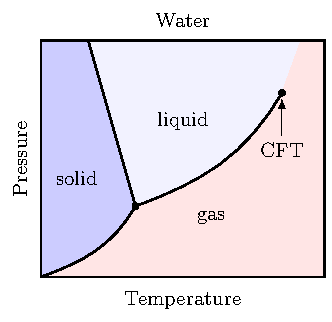
\includegraphics[]{Lectures/Figures/PT_diagram.pdf}
    \caption{Phase diagram of water. There is a lot of rich phenomenology in the phase transitions, for example at the critical point where the system is scale invariant and described by a CFT.}
    \label{fig:PTwater}
\end{figure}

In the magnet case, we can have magnetic and non-magnetic phase. In magnetic phase, has to choose a direction for the magnetization to point in. This breaks the $\ZZ_2$ symmetry. Looking at the phase diagram for a magnet, we have the parameters $T$ temperature and $h$ the external magnetic field. For $h > 0$ we have magnetization up and for $h < 0$ we have magnetization down. At zero temperature the transition is abrupt. There is a critical temperature $T_c$ above which the transition is smooth, and below $T_c$ we have varying degrees of an abrupt transition. Interestingly, the critical point between liquid and gas ``looks like'' an Ising transition.

\begin{figure}[htbp!]
    \centering
    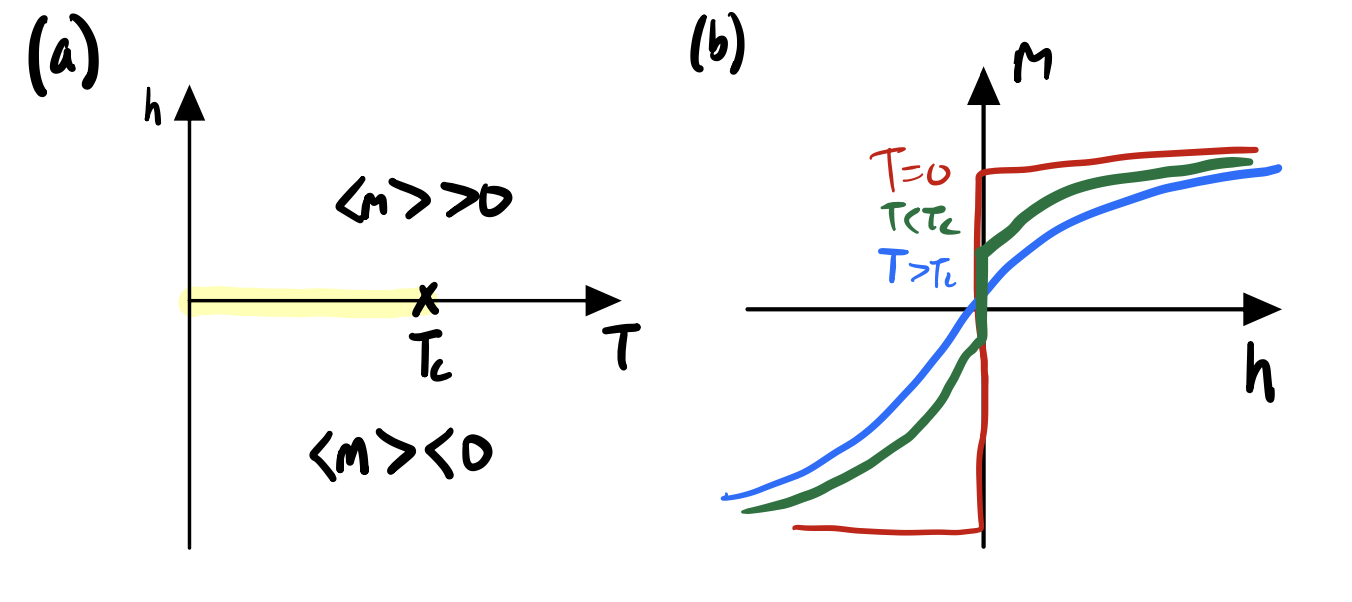
\includegraphics[scale=0.55]{Lectures/Figures/Ising_phases.png}
    \caption{(a)$h$ (external field) vs. $T$ (temperature) phase diagram for the Ising model and (b) behaviour of $m$ (magnetization) as a function of $h$ for different $T$. For $h > 0$ we have $\avg{m} > 0$ and vise versa for $h < 0$. For $T < T_c$, there is an abrupt transition in $m$ at $h=0$ (yellow line). This can be seen by studying the behaviour of $m$ for different temperatures; for $T = 0$ the transition is abrupt (as we would expect; since the external field is the only contribution to the energy, any finite magnetic field fully polarizes the spins). Below $T_c$ the transition stays abrupt, though with a smaller ``jump'' in the magnetization, and above $T_c$ the transition is smooth.}
    \label{fig:Ising_phases}
\end{figure}

We can obtain scaling laws for the magnetization:
\begin{equation}
    m(T, h = 0) = \begin{cases} 0 & T > T_c \\ \abs{t}^\beta & T< T_c \end{cases}
\end{equation}
\begin{equation}
    m(T = T_c, h) \sim h^{1/\delta}
\end{equation}

There are other quantities we may compute; for example we could measure the magnetic susceptibility $\chi = \dpd{m}{h}(t)$. Because the system becomes very polarizable near the phase transition, we may expect that $\chi$ has a peak/divergence at $T = T_c$, which is characterized by a further exponent. We could also compute the specific heat of the system, which also has its associated exponent and so on.

There's a whole zoo of critical exponents, and it turns out that there are (universality) classes where the exponents are the same - i.e. near these phase transitions very different systems are governed by the same theories.

Note that the theory described by Eq. \eqref{eq:GinzLandau} is known as Ginzburg-Landau theory (or the \emph{mean-field} theory), and was written down to describe phenomenology. We have a power series expansion in the magnetization, with the coefficients (e.g. $a$) as smooth functions governed by $T, h$, and so on.

We can consider a $\phi^4$ theory:
\begin{equation}
    F = a\phi^2 + b\phi^4 + h\phi
\end{equation}
with a phenomenological guess of $a = a_0(T - T_c)$.
\begin{equation}
    \dod{F}{\phi} = 0, \quad \phi^2 = -\frac{a}{b} \text{ or } \phi = 0
\end{equation}
We then have $\phi \sim (T_c - T)^{1/2}$, i.e. $\beta = 1/2$.

General procedure: Start with mean field theory. Then, aspects of field theory will turn out. One aspect will be thermal fluctuations about the mean field theory states. Then we think about terms like $k(\nabla m)^2$, which tells us that there are energy costs to (e.g.) mis-aligned spins. This is known still as the Gaussian model as the Hamiltonian with this term is still quadratic in the fields. The moment I have a gradient term, I get modes in the system that can propagate. If I have a lot of modes, I don't get a phase transition.

Scaling Hypothesis - I know there are a set of critical exponents. How are they related? Via scaling. So, suppose I look at the system on different scales. As I average over different scales, if the system has to look self-similar. RG gives us a way to obtain critical exponents.

Other systems - we will also look at systems in low-dimensions, which can be interesting. There are also systems with inherent disorder/randomness, e.g. glasses which are frozen but not ordered systems. There is at least one model that realizes this, which Parisi got a Nobel for. We will also look at dynamical systems; what happens to open/driven systems? There are ways to formally write them in a very similar language. E.g. friction, forced flow, growing things at an interface, biology. Finally, we may study information and data. The straightforwards introduction for physicists is spin glasses, which can (in theory) be used to encode data via learning a set of interactions $J_{ij}$. 
\section{From Particles to Fields}
In this lecture, we will look at a chain of atoms, and a chain of ferromagnetic spins.

\subsection{Phonons}

We consider atoms of mass $m$ connected by springs of spring constant $k_s$, with equilibrium $a$. We can notate the displacement of the $n$th atom from its equilibrium position as $\phi_n$, and $x_n$ the distance of the $n$th atom from the end of the string. 

\begin{figure}[htbp]
    \centering
    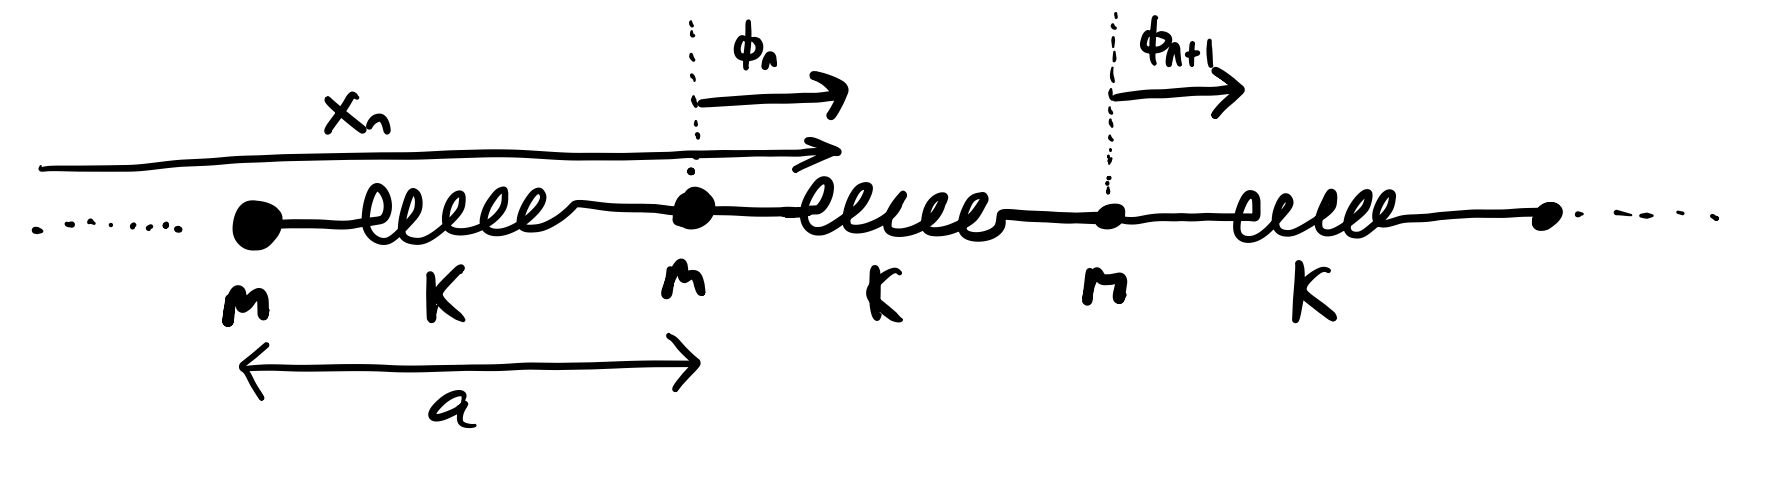
\includegraphics[scale=0.4]{Lectures/Figures/Atom_spring_chain.png}
    \caption{Diagram of a chain of atoms connected by springs.}
    \label{fig:Atom_spring_chain}
\end{figure}

The Lagrangian of the system is then:
\begin{equation}
    L = T - V = \sum_{i=1}^N \left[\frac{1}{2}m\dot{x}_n^2 - \frac{k_s}{2}\left(x_{n+1} - x_n - a\right)^2\right] = \sum_{n=1}^N \left[\frac{1}{2}m\dot{\phi}_n^2 - \frac{k_s}{2}\left(\phi_{n+1}-\phi_n\right)^2\right]
\end{equation}
notice there is a potential energy piece and a kinetic energy piece, both quadratic. We will want to solve for the eigenmodes of these problem. There are $N$ degrees of freedom and as such we expect to find $N$ eigenmodes.

This problem is solvable! We can write down the equation of motion of the springs; this is just nearest neighbour couplings so we can write down an analytic solution.

We promote:
\begin{equation}
    \phi_n \to a^{1/2}\phi(x)
\end{equation}
with the $a^{1/2}$ introduced for dimensional purposes, namely in such a way that we measure position in units of $\frac{x}{a}$, i.e. making it dimensionless. Then:
\begin{equation}
    (\phi_{n+1} - \phi_n) \to a^{3/2}\p_x \phi(x)
\end{equation}
Finally, we convert from a discrete sum to an integral:
\begin{equation}
    \sum \to \frac{1}{a}\int_0^{L=N_a}dx
\end{equation}
Thus the Lagrangian becomes a \emph{functional} (i.e. a function of a function) of a field:
\begin{equation}
    L[\phi] = \int_0^x \mathcal{L}(\phi, \p_x\phi, \dot{\phi})
\end{equation}
where $\mathcal{L}$ is the Lagrangian density:
\begin{equation}
    \mathcal{L} = \frac{1}{2}m\dot{\phi}^2 - \frac{k_s a^2}{2}(\p_x \phi)^2.
\end{equation}
We then write down the classical action:
\begin{equation}
    S[\phi] = \int dt L[\phi]
\end{equation}
Currently the field $\phi$ is not determined; it is a function of $x, t$. Our next task is to look for solutions that minimize the action.

To this end, we have the Euler-Lagrange equation:
\begin{equation}
    \dpd{\LL}{\phi} - \dod{}{t}\dpd{\LL}{\dot{\phi}} - \dod{}{x}\dpd{L}{(\p_x \phi)} = 0
\end{equation}
which is derived from the principle of least action. Working out the Euler Lagrange equation, we get the expected result:
\begin{equation}
    \boxed{[m\p_t^2 - (k_s a^2)\p_x^2]\phi(x, t) = 0}
\end{equation}
this is a wave equation! What we can see is it describes sound waves. Notice that the above equation is translation invariant, and as such the general solution is the sum of a right and left handed wave:
\begin{equation}
    \phi_+(x + vt) - \phi_-(x - vt)
\end{equation}
with velocity:
\begin{equation}
    v = a\sqrt{\frac{k_s}{m}}.
\end{equation}

Often however, it is common to look at this equation and say that it is simplest to study it in terms of Fourier modes; consider solutions:
\begin{equation}
    \phi(x, t) = \phi_0e^{i(\omega t - kx)}
\end{equation}
which plugging into the wave equation gives us the dispersion relation:
\begin{equation}
    \omega = vk
\end{equation}
The waves oscillate in time and in space.

Going back to the discrete case, we have the eigenmodes:
\begin{equation}
    \phi_n(t) = \sum_{k}\frac{1}{\sqrt{N}}e^{i(\omega_k t - k n a)}
\end{equation}
with dispersion:
\begin{equation}
    \omega(k) = 2\sqrt{\frac{k_s}{m}}\abs{\sin(\frac{k a}{2})}
\end{equation}
This solution knows about the discreteness of the lattice. Going to the continuum, we lost something, but we have a much simpler theory. In particular, the theory is good for small $k$/large wavelengths. The coarse graining made us lose information about the short-wavelength modes; we should not use the field theory for microscopic wavelengths. But, say for populating the chain with low-$T$ bosons (i.e. low energy bosons) this captures the phenomenology well. 

The dispersion curves looks like:
\begin{figure}[htbp]
    \centering
    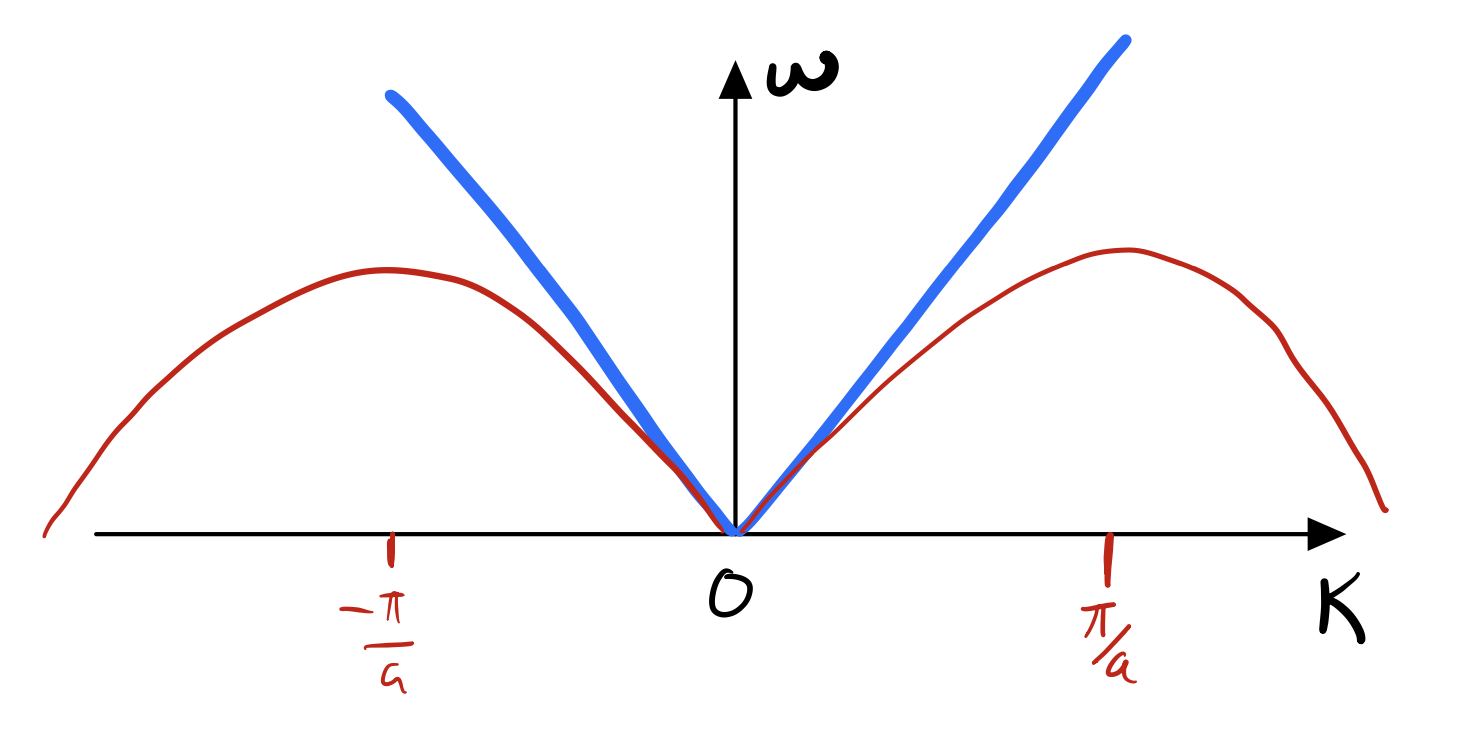
\includegraphics[scale=0.4]{Lectures/Figures/Phonon_dispersion.png}
    \caption{Continuum and Discrete Dispersion. The continuum dispersion is linear in $k$, while the discrete dispersion is $\sim \abs{\sin(k)}$. The two dispersion relations agree for small $k$/large wavelengths/small energies.}
    \label{fig:Phonon_dispersion}
\end{figure}

We can now use this to do thermodynamics! We can write down the internal energy:
\begin{equation}
    E(T) = E_0 + \sum_k \hbar \omega(k)\left[\avg{n_k} + \frac{1}{2}\right]
\end{equation}
where:
\begin{equation}
    \avg{n_k} = \frac{1}{e^{\frac{\hbar\omega}{k_BT}} - 1}
\end{equation}
In the limit where $k_B T \ll \hbar\omega$, $\hbar\omega(k) \to \hbar v k$ and the energy goes as $\sim T^2$. This is the well known thermodynamic dependence of the spring chain.

\subsection{Ferromagnetic Heisenberg Chain}
We consider the quantum Hamiltonian:
\begin{equation}
    \hat{H} = -J\sum_{m=1}^{N-1} \hat{\v{S}}_m \cdot \hat{\v{S}}_{m+1}
\end{equation}
where we take the coupling $J > 0$ such that the spins aligning result in lowered energy (i.e. we are describing a ferromagnet). At each site we have spin operators:
\begin{equation}
    [\hat{S}^i_m, \hat{S}^j_n] = i\delta_{mn}\e^{ijk}\hat{S}^k_n
\end{equation}
with $\delta_{mn}$ the Kronecker delta (which tells us that the spin operators only have nontrivial commutation on the same site) and $\e^{ijk}$ is the totally anti-symmetric tensor. We denote the total spin as $S$, a number (can be 1/2, 1, 3/2, etc.). We can consider the eigenstates of $\hat{S}^z$:
\begin{equation}
    \hat{S}^z_m\ket{s_m} = s\ket{s_m}.
\end{equation}
where $\ket{S_m}$ form a ladder of states from $s = -S, -S+1, \ldots, S-1, S$. We guess the ground state:
\begin{equation}
    \ket{\Omega} = \bigotimes_{m=1}^N \ket{S_m}
\end{equation}
i.e. all the spins are spin up. This clearly minimizes the energy, as for each coupling term $\v{S}_m \cdot \v{S}_{m+1}$ we get energy $-JS$ and so the total energy of $\ket{\Omega}$ is $-JSN$. Note however in writing this ground state down we broke some symmetry, as indeed the spins could be all aligned in any direction, and we would get the same ground state energy.

Recall that on a single site, we can have the raising/lowering operators:
\begin{equation}
    \hat{S}^\pm_m = \hat{S}^x_m \pm i \hat{S}^y_m
\end{equation}
which takes us up/down the ladder of $\ket{s_m}$ eigenstates. We can now rewrite our Hamiltonian to be of the form:
\begin{equation}
    \hat{H} = -J\sum_m \left(\hat{S}^z_m\hat{S}^z_{m+1} + \frac{1}{2}\left(\hat{S}^+_m\hat{S}^-_{m+1} + \hat{S}^-_m\hat{S}^+_{m+1}\right)\right)
\end{equation}

We now play a trick, namely the Holstein-Primakoff transformation. We define new operators (sometime known as magnon variables):
\begin{equation}
    \hat{S}^z_m = S - \hat{a}^\dag_m \hat{a}_m
\end{equation}
\begin{equation}
    \hat{S}^+_m = \left(2S - \hat{a}^\dag_m \hat{a}_m\right)^{1/2}a
\end{equation}
\begin{equation}
    \hat{S}^-_m = \hat{a}^\dag_m \left(2S - \hat{a}^\dag_m \hat{a}_m\right)^{1/2}
\end{equation}
where:
\begin{equation}
    [\hat{a}_m, \hat{a}_n^\dag] = \delta_{mn}
\end{equation}
It can be verified that this transformation is \emph{exact} (though it looks strange!) as it preserves the spin commutation relations. Why does this work? Intuitively, we have introduced the bosons through the operators $\hat{a}, \hat{a}^\dag$; the ladder of spin states look like the ladder of spin states (just that one is an infinite, and one is a finite ladder). But the square roots actually make sure that the dimensionality of our Hilbert space is preserved, because when I hit the walls of $\pm S$, the state vanishes. However it is instructive to consider the case where $S$ is large:

Let us Taylor expand $\hat{S}^\pm$:
\begin{equation}
    \hat{S}^+_m \approx \sqrt{2S}\hat{a}_m + \frac{O(\hat{a}_m^\dag \hat{a}_m \hat{a}_m)}{\sqrt{2S}}
\end{equation}
if $S \to \infty$, then we can throw away all but the first order term. Interestingly, it has a habit of working even when $S = \frac{1}{2}$. Let us write the Hamiltonian to second order in the operators:
\begin{equation}
    \hat{H} = -JNS^2 + JS\sum_m\left[\hat{a}^\dag_m\hat{a}_m + \hat{a}^\dag_{m+1}\hat{a}_{m+1} - \hat{a}^\dag_m \hat{a}_{m+1} - \hat{a}^\dag_{m+1}\hat{a}_m\right] + O(S^0)
\end{equation}
The number operator terms come from the $\hat{S}^z$, while the exchange terms come from the $\hat{S}^\pm$ cross terms. As such, we have now rewrote the Hamiltonian in terms of bosonic modes. Because this is periodic, the natural thing to do is to go back to the phonon problem in the discrete sense. There, we went into momentum space, and we shall do that again here:
\begin{equation}
    \tilde{\hat{a}}_k = \frac{1}{\sqrt{N}}\sum_m e^{ikm}\hat{a}_m
\end{equation}
where the $\tilde{\hat{a}}_k$ corresponds to a momentum annihilation operator and $\hat{a}_m$ corresponds to a position annihilation operator. Note that the momentum operators obey the same algebra:
\begin{equation}
    [\tilde{\hat{a}}_k, \tilde{hat{a}}^\dag_{k'}] = \delta_{kk'}
\end{equation}
which transforms the Hamiltonian into:
\begin{equation}
    \hat{H} = -JNS^2 + \sum_k \omega_k \tilde{\hat{a}}^\dag_k \tilde{\hat{a}}_k
\end{equation}
where:
\begin{equation}
    \omega_k = 4J\sin^2(\frac{k}{2})
\end{equation}
This is a quadratic (at small $k$) dispersion relation. Note that we still have a zero mode at $k = 0$ where the symmetry is preserved. Note also that in the HW, you will solve the classical version of this problem, and find the same dispersion.

\begin{figure}[htbp]
    \centering
    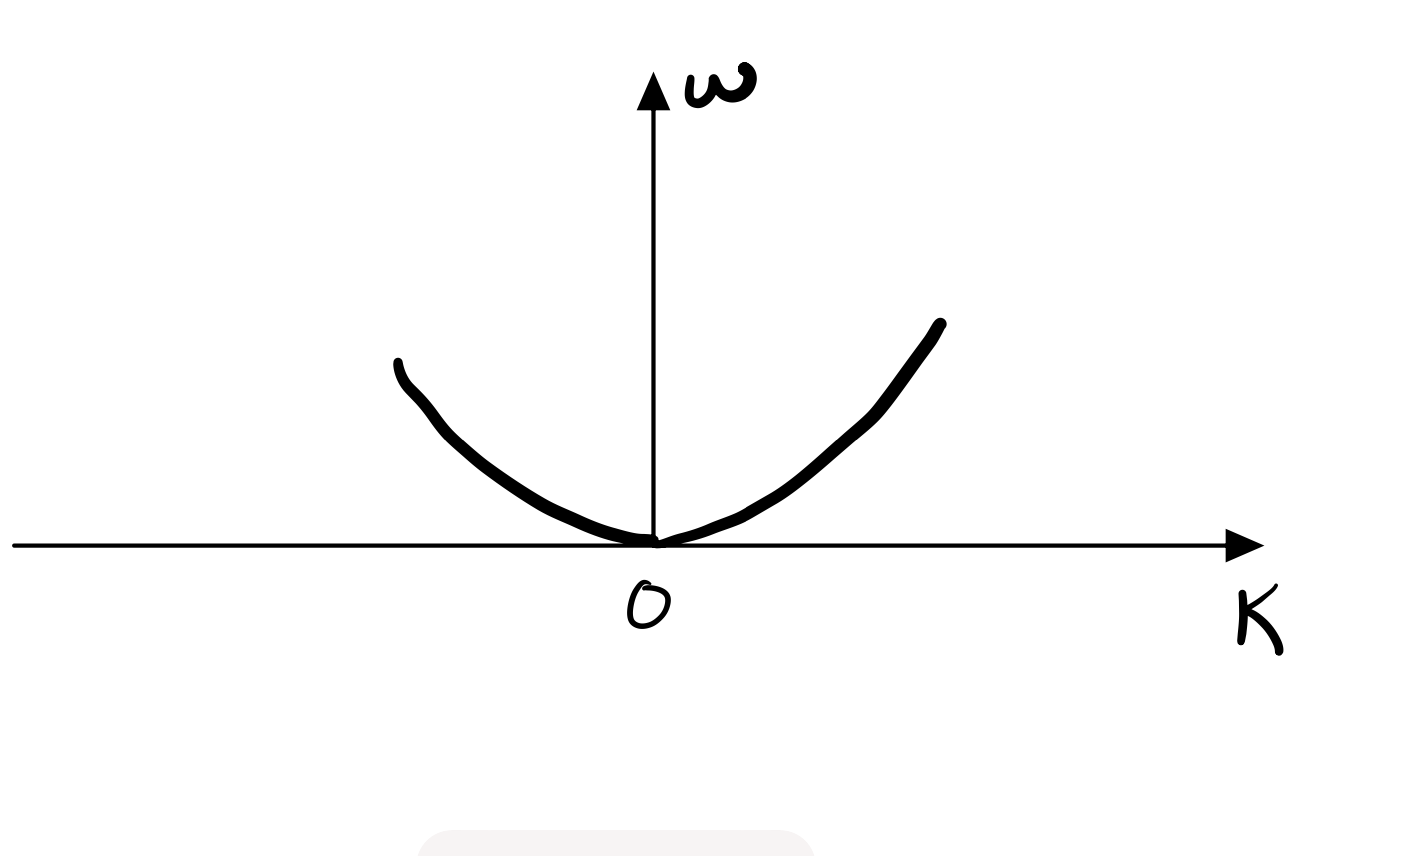
\includegraphics[scale=0.4]{Lectures/Figures/FM_spin_dispersion.png}
    \caption{Small $k$ dispersion relation for the ferromagnetic Heisenberg spin chain. For small $k$, the dispersion is quadratic.}
    \label{fig:FM_spin_dispersion}
\end{figure}

We call these objects ``spin waves''. This is clearly an approximation, as we have ignored the $O(S^0)$ terms in the Hamiltonian which include terms such as $\hat{a}^\dag a \hat{a}^\dag a$ which correspond to interactions between spin waves. So long as we stay near the zero mode, there is ``nowhere to go'' so the interactions can be neglected (if we look at large $k$ modes on the other hand, the interactions become relevant). 

A naive field theory for this would produce $\omega_k \sim k$, but it turns out spin conservation + rotational invariance gives us $\omega_k \sim k^2$. On Friday, we will look at the antiferromagnetic version of this problem, where we will see we obtain $\omega_k \sim k$ (due to vacuum fluctuations).

\section{Antiferromagnetic Heisenberg Chain,}
\subsection{Review of the Heisenberg Chain}
Recall the Heisenberg spin chain Hamiltonian:
\begin{equation}\label{eq:Heisenbergchain}
    \hat{H} = -J\sum_m\left(\hat{S}^z_m\hat{S}^z_{m+1} + \frac{1}{2}\left(\hat{S}^+_m\hat{S}^-_{m+1} + \hat{S}^-_m \hat{S}^+_{m+1}\right)\right)
\end{equation}
and after the Holstein-Primakoff transformation, this became:
\begin{equation}
    \hat{H} = -JNS^2 + JS\sum_{m}\left(\hat{a}^\dag_m\hat{a}_m + \hat{a}^\dag_{m+1}\hat{a}_{m+1} - \hat{a}^\dag_m\hat{a}_{m+1} - \hat{a}^\dag_{m+1}\hat{a}_m\right) + O(S^0)
\end{equation}
Note to get here we first did an exact transformation into bosonic operators, then expanded this transformation in a Taylor series to obtain a Hamiltonian quadratic in $\hat{a}/\hat{a}^\dag$. This can be turned into a field theory; loosely, we can replace the $a$s by field operators:
\begin{equation}
    \hat{a}_m \to \hat{\phi}(x), \quad \hat{a}^\dag_m \to \hat{\phi}^\dag(x)
\end{equation}
Further, we can consider:
\begin{equation}
    \hat{a}_{m+1} \approx \hat{a}_m + \dpd{}{x}\hat{a}_m
\end{equation}
which can give us $\nabla \hat{\phi}$ terms. We also have the promotion of the commutators to the continuum:
\begin{equation}
    [\hat{a}_m, \hat{a}^\dag_{m'}] = \delta_{mm'} \to [\hat{\phi}(x), \hat{\phi}^\dag(x')] = \delta(x - x')a
\end{equation}
Note that this would give us a free field theory (as the bosonic operator terms are all quadratic).

\subsection{Antiferromagnetic Case}
Formally, we change the sign of $J$ in Eq. \eqref{eq:Heisenbergchain} so that it is now $J < 0$. Now, we guess our ground state to be alternating between spin up/down, with spins on the A sublattice being up and those on the B sublattice being down:

\begin{figure}[htbp]
    \centering
    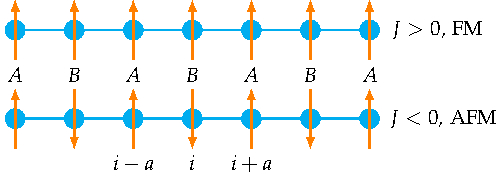
\includegraphics[scale=0.5]{Lectures/Figures/FMAFMHeisenbergchain.pdf}
    \caption{Cartoon picture of FM and AFM Heisenberg chain. $J > 0$ (ferromagnet) encourages the spins to align, while $J < 0$ (antiferromagnet) encourages the spins to anti-align. Our guess for the ground state in this case is to bipartition the chain into two sublattices, $A, B$ for spins pointing up and down. We do note that this is an ansatz/guess for the ground state, and is not an exact eigenstate of the quantum Hamiltonian.}
    \label{fig:FMAFMHeisenbergchain}
\end{figure}
So, let us consider applying a $\pi$ rotation on the $B$ sublattice of spins, i.e. taking:
\begin{equation}
    S^z_B \to -S^z_B, \quad S^y_B \to -S^y_B, \quad S^x_B \to S^x_B
\end{equation}
So the Hamiltonian becomes:
\begin{equation}\label{eq:AFMHeisenbergchain}
    \hat{H} = -\abs{J}\sum_m\left(\hat{S}^z_m\hat{S}^z_{m+1} - \frac{1}{2}\left(\hat{S}^+_m\hat{S}^+_{m+1} + \hat{S}^-_m \hat{S}^-_{m+1}\right)\right)
\end{equation}
or with the H.P. transformation:
\begin{equation}\label{eq:AFMHeisenbergchainHP}
    \hat{H} = -\abs{J}NS^2 + \abs{J}S\sum_{m}\left(\hat{a}^\dag_m\hat{a}_m + \hat{a}^\dag_{m+1}\hat{a}_{m+1} - \hat{a}_m\hat{a}_{m+1} - \hat{a}^\dag_{m+1}\hat{a}^\dag_m\right) + O(S^0)
\end{equation}
If we diagonalize this (which we can always do - it is a quadratic form!) we obtain:
\begin{equation}
    \hat{H} = -N\abs{J}S(S+1) + \abs{J}S\sum_k \m{\hat{a}^\dag_k & \hat{a}_k}\m{1 & \cos k \\ \cos k & 1} \m{\hat{a}_{-k} \\ \hat{a}^\dag_{-k}}
\end{equation}
where:
\begin{equation}
    \hat{a}_k = \sum_m e^{ikm}\hat{a}_m
\end{equation}
Now doing a Bogoulibov transformation:
\begin{equation}
    \m{\hat{\alpha}_k \\ \hat{\alpha}^\dag_{-k}} = \m{\cosh \theta_k & -\sinh \theta_k \\ -\sinh\theta_k & \cosh\theta_k}\m{\hat{a}_k \\ \hat{a}^\dag_{-k}}
\end{equation}
with $\tanh 2\theta_k = \cos k$. With this rotation, $\hat{H}$ becomes:
\begin{equation}
    \hat{H} = -N\abs{J}S^2 + 2\abs{J}S\sum_k(\sin k)\hat{\alpha}^\dag_k \hat{\alpha}_k
\end{equation}
Which gives us the spectrum - it is linear! We can think of these eigenstates as linear superpositions of spin waves in the original basis.

Unfortunately, we aren't quite done. These operators are not conserved. Because the ground state is defined by $\hat{\alpha}_k\ket{0} = 0$, but $\hat{\alpha}_k$ is a combination of $a^\dag/a$s and so can create excitations.

Let us look at the magnetization of the ground state:
\begin{equation}
    M = \bra{0} \frac{1}{N}\sum_i \hat{S}^z_i\ket{0} = S - \frac{1}{N}\sum_i \bra{0}a^\dag a \ket{0} = S - \frac{1}{N}\sum_k \sinh^2\theta_k
\end{equation}
I.e. we see it is nonzero! These are quantum fluctuations on top of the classical ground state. Looking at the integral form for this, we have:
\begin{equation}
    M = S - \int_0^{1/a}dk \frac{1}{k} k^{d-1}
\end{equation}
which diverges at $k = 0$ for $d = 1$. An important note to make; fluctuations, even quantum ones, can destroy phase transitions! E.g. the 1D classical Heisenberg model orders, the quantum one does not. But of course when we look at thermal fluctuations thing disorder even more.

The fact that $M$ diverges in 1D tells us that the approximation (i.e doing the sublattice divisions...) we made at the beginning was incorrect. This sublattice division is incorrect as there is no local $SU(2)$ symmetry (only a global one). This might have been okay if I was just asking about long range order. If $M$ turned out to be finite, we would still have a magnet... but here that is not the case.

\subsection{Phase Transitions in the Classical Magnet}
We consider a classical magnet (i.e. a lattice of classical spins), subject to two parameters, an external magnetic field $h$ and a temperature $T$. We consider the magnetization $m(T)$, which is something we may measure in a lab:
\begin{equation}
    m(T) = \frac{1}{V}\lim_{h \to 0}M(h, t)
\end{equation}
where:
\begin{equation}
    M(h, T) = \frac{1}{N}\sum_i S_i
\end{equation}
is a quantity that depends on the external field and temperature.

We have the scaling of the magnetization:
\begin{equation}
    m(T, h=0) = \begin{cases}
        0 & t > 0
        \\ \abs{t}^\beta & t < 0
    \end{cases}
\end{equation}
with $t = \frac{T_c - T}{T}$. We can also consider the scaling of $m$ w.r.t. $h$ at the critical temperature:
\begin{equation}
    m(T = T_c, h) \propto h^{1/\delta}.
\end{equation}
The $\beta, \delta$ appearing above are the critical exponents that quantify the phase transition.

We may also consider the measurement of a response function, i.e. the response of the system to some perturbation that we put in. An example is the magnetic susceptibility $\chi$:
\begin{equation}
    \chi(T, h =0) = \dpd{m}{h}
\end{equation}
or the specific heat:
\begin{equation}
    C = \left.\dod{E}{T}\right|_T \propto c \abs{t}^{-\alpha_\pm}
\end{equation}

\begin{figure}
    \centering
    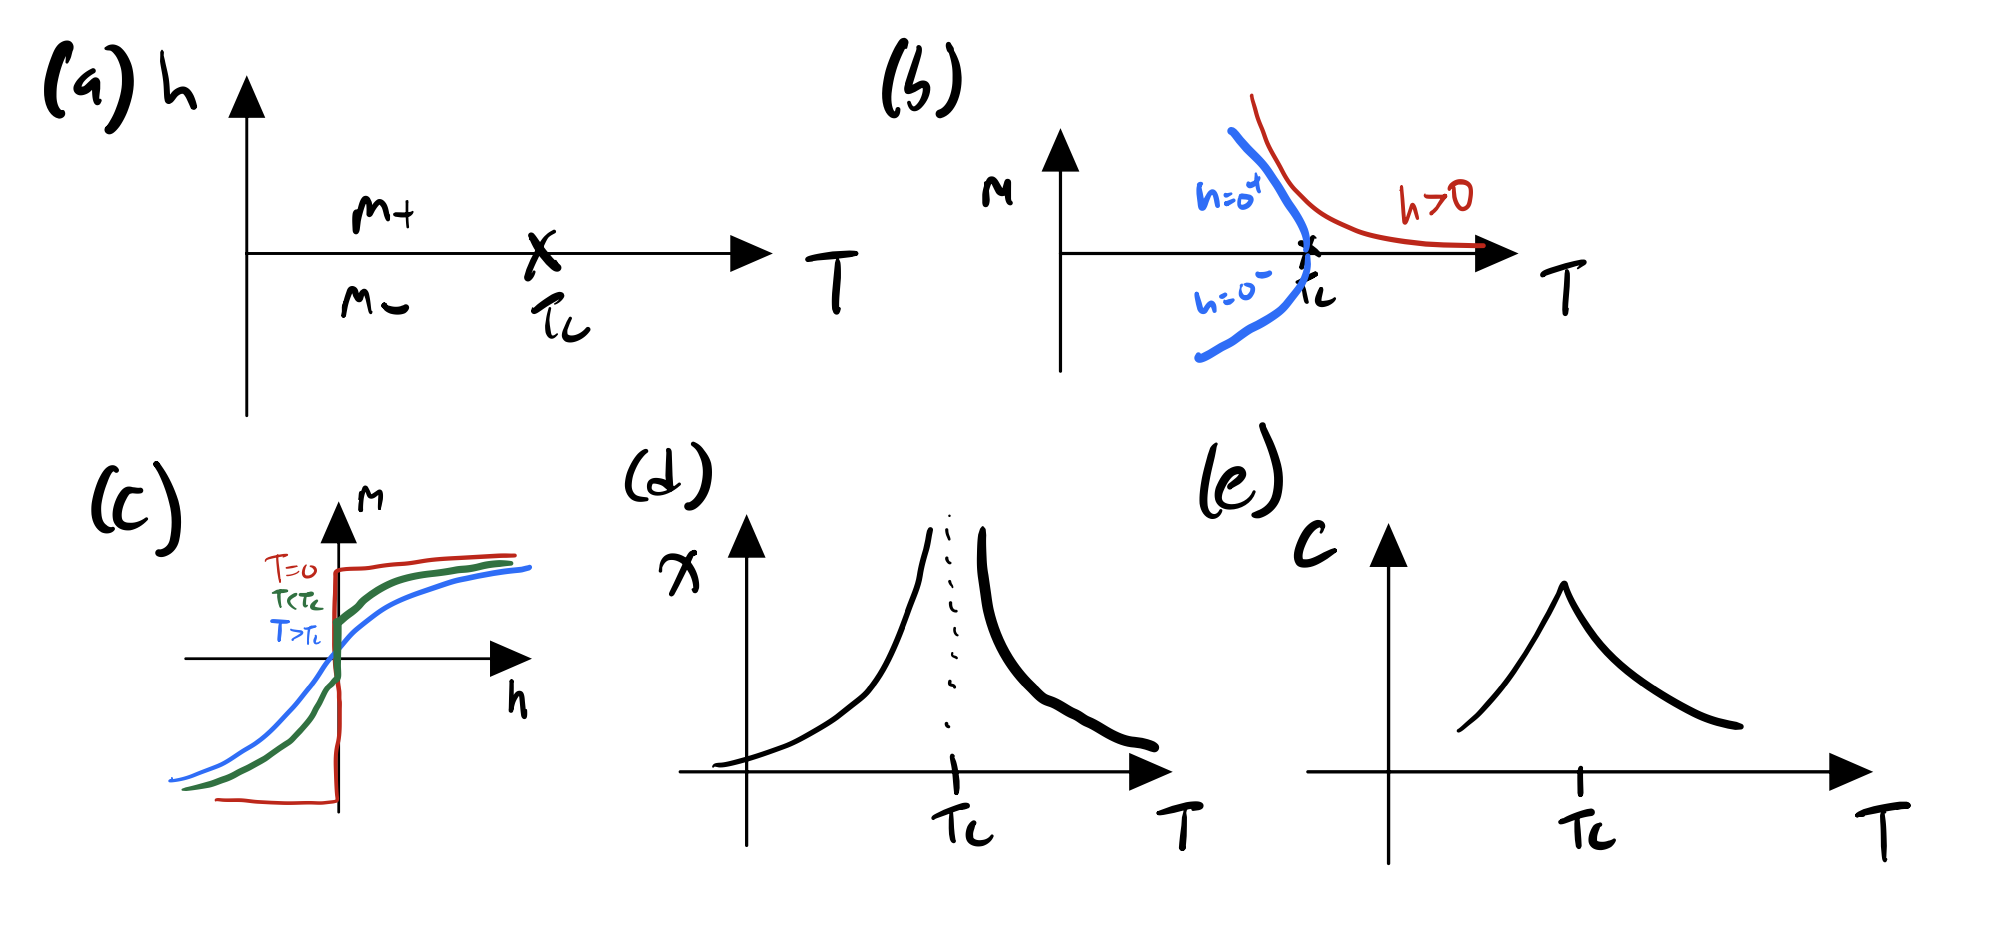
\includegraphics[scale=0.5]{Lectures/Figures/Various_plots.png}
    \caption{Plots of various measurable quantities and their behaviours near the critical temperature. (a) External field vs. Temperature. (b) Magnetization vs. Temperature for $h = 0$ and $h > 0$. (c) Magnetization vs. External field for various $T$. (d) Magnetic susceptibility vs. Temperature. (e) Heat capacity vs. Temperature.}
    \label{<label>}
\end{figure}

How do we calculate these quantities? We start with some partition function:
\begin{equation}
    Z = \Tr (e^{-\beta(H_0 + m.h.)})
\end{equation}
with $\beta = (k_B T)^{-1}$, $H_0 = -J\sum_{ij}S_iS_j$ and $m.h. = -h\sum_i S_i$ (the magnetization in field $h$). The trace here is a shorthand to say we compute the exponential for every possible configuration of spins, with the terms weighted by the energy (you could do this numerically, e.g. by doing a Monte Carlo simulation).

If I have a partition function, I can compute things! In particular, if I want to compute the (average) magnetization:
\begin{equation}
    \avg{M} = \dpd{\ln Z}{(\beta h)} = \frac{1}{Z}\Tr(Me^{-\beta(H_0 + m.h.)})
\end{equation}
We can then compute $\chi$:
\begin{equation}
    \chi = \dpd{M}{h} = \beta\left[\frac{1}{Z}\Tr\left(M^2e^{-\beta H}\right) - \frac{1}{Z^2}\left(\Tr(Me^{-\beta H})\right)^2\right]
\end{equation}
Of we look at this carefully, we see the first term is the expectation of $M^2$ and the second term is the square of the expectation value of $M$, i.e.:
\begin{equation}
    \chi = \beta\left(\avg{M^2} - \avg{M}^2\right).
\end{equation}
Thus, the susceptibility tells you about fluctuations from the average.

This $M$ we have written here is an average over all configurations and over all space. We may also be interested in an average just over space. To this end, we may consider that the macroscopic magnetization is just the integral over the course-grained position dependent magnetization $m(x)$:
\begin{equation}
    M = \int d^3r m(x)
\end{equation}
from which:
\begin{equation}
    \chi = \beta \int d^3r d^3r' \left(\avg{m(r)m(r')} - \avg{m(r)}\avg{m(r')}\right).
\end{equation}
Now, if $r, r'$ are closeby, we expect the magnetization to be correlated, and if they are not, it depends on the ordering of the state. To this end, let us define here a connected average of $C$:
\begin{equation}
    \avg{m(r)m(r')}_C = \avg{(m(r) - \avg{m(r)})(m(r') - \avg{m(r')})} = G(r-r') - m^2
\end{equation}
where $G$ is a (Green's) function that depends on the distance $r-r'$. With this, the integral for $\chi$ becomes:
\begin{equation}
    \chi = \frac{V}{k_B T}\int dr \avg{m(r)m(0)}_C.
\end{equation}
So, interestingly, the susceptibility tells us something about the correlation function of spins. Generically, I expect this to decay:
\begin{equation}
    G(r) \sim e^{-r/\xi}
\end{equation}
which introduces the idea of a correlation length $\xi$. As I approach the phase transition, far-away degrees of freedom become more and more correlated- from the divergence of $\chi$ at the phase transition, we can also conclude that the correlation length $\xi$ must also diverge. Thus, we hypothesize:
\begin{equation}
    \xi \sim \abs{t}^{-\nu}.
\end{equation}
Also, notice that this happens on \emph{both} sides of the transition.

\subsection{Ginzburg-Landau Theory}
Another way we can thing about the partition function:
\begin{equation}
    Z(T) = \Tr(e^{-\beta H}) = \int \mathcal{D}[m(r)] W(m(r))
\end{equation}
I.e. look at all spatial configurations $\mathcal{D}[m(r)]$ of the order parameter, for each of these compute the statistical weight $W$, and add them up. 

We can use the $W$ to define a Hamiltonian:
\begin{equation}
    \beta H[m(r)] = -\ln W[m(r)]
\end{equation}
we do this to avoid writing down a microscopic Hamiltonian. Then, $\beta H[m(r)]$ is a functional of $m$, so:
\begin{equation}
    \beta H[m(r)] = \int d^dr \phi[m(r), r] = \int d^d r \phi[m, \nabla m, \nabla^2m, h, \ldots]
\end{equation}
We assume that $\phi$ is an analytic function of all of these variables, and stop at some point because we would consider some terms to not be relevant.
\section{Ginzburg-Landau Theory Continued}
\subsection{Review from last class + Symmetries}
We will go into the phenomelogical G-L theory, showing how the mean field theory are derived from the saddle point approximation. We then consider small Gaussian fluctuations about this saddle point. Sometimes these fluctuations are not actually small, which will get us into discussion of the renormalization group.

We start with the partition function:
\begin{equation}
    Z(T) = \Tr(e^{-\beta H}) = \int \mathcal{D}[\bar{m}(\v{r})]W(\bar{m}(\v{r}))
\end{equation}
Here, $\bar{m}$ is a coarse-grained averaged of the order parameter, the coarse-grained version of the microscopic spins $S_i$s. We take an integral over all configurations, and we associate with each configuration a statistical weight $W$.

We then define the (effective) Hamiltonian as:
\begin{equation}
    \beta H_{\text{eff}}[\bar{m}(\v{r})] = -\ln W[\bar{m}(\v{r})] \implies W \sim e^{-\beta H_{\text{eff}}}
\end{equation}
We remark that RG will eventually allow us to derive the effective Hamiltonian from the microscopic one. Then, $\beta H[\bar{m}(\v{r})]$ is a functional of $m$, and we assume that $\Phi$, whose integral gives the effective Hamiltonian, is local:
\begin{equation}
    \beta H_{\text{eff}} = \int d^dr \Phi[\bar{m}(\v{r}), \v{r}]
\end{equation}
and then we may expand it perturbatively:
\begin{equation}
    \Phi[\bar{m}(\v{r}), \nabla \bar{m}(\v{r}), \nabla^2 \bar{m}(\v{r}), \ldots].
\end{equation}
The next assumption that $\Phi$ is an analytic function. We now consider symmetries of the system. For example for the Heisenberg chain, we have rotational symmetry:
\begin{equation}
    H[R\bar{m}] = H[\bar{m}]
\end{equation}
This symmetry implies that the leading order term must be $\bar{m}^2 = \bar{\v{m}}\cdot\bar{\v{m}}$, and then $\bar{m}^4$ and so on (the rotational symmetry forbids odd powers). Further, inversion symmetry forbids odd powers in $\nabla m$, so we consider:
\begin{equation}
    (\nabla \bar{m})^2 = \sum_{i=1}^n \sum_{\alpha=1}^d (\p_\alpha \bar{m}_i)(\p_\alpha \bar{m}_i)
\end{equation}
What if the system is anisotropic? E.g. we have a unit cell that has different $x/y$ lengths; then we can rescale via redefinition $y \to yb, x \to x/a$ to recover isotropy. The symmetries must then be preserved.

\subsection{Minimal Model}
We consider a scalar field $m$, where:
\begin{equation}
    \beta H = \text{const} + \int d^dr\{\frac{1}{2}tm^2(\v{r}) + \frac{1}{4}um^4(\v{r}) + \frac{1}{2}k(\nabla m)^2 - hm\}
\end{equation}
Where we note the model has inversion symmetry up to the external magnetic field term. At the moment, the constants appearing in the model are all phenomelogical, e.g. $t = t(T, B, P, \ldots)$ For now, we don't care about the parameters precisely - we are just trying to see if there is any interesting behaviour generically interesting in theory. Are there any points in parameter space where it changes its behaviour? This is quite a different approach from trying to ``solve'' a specific microscopic model.

For this theory to be sensible, we must have $u > 0$; else the magnetization will grow to infinity (as $m \to \infty$ would then prove to be the lowest energy configuration), and there is nothing to stabilize the model (if $u < 0$ we require a $m^6$ term to stabilize it). $k > 0$ is also known from the phonons in the model; it gives the dispersion at long wavelengths; if $k < 0$, it would disperse downwards, and at finite wavevectors the model would be unstable.

\subsection{Mean Field Theory from Saddle Point Approximation}

The next question - a technical one - is what does $\mathcal{D}[m(\v{r})]$ mean? The idea will be to discretize:
\begin{equation}
    \int D[m] F(m, \dpd{m}{x}, \ldots) = \lim_{N \to \infty}\prod_{i=1}^N \int dm_i F[m_i, \frac{m_{i+1} - m_i}{\delta}, \ldots]
\end{equation}
Large fluctuations have a high energy cost (due to the gradient term) and thus have low statistical weight. 

The first thing we are tempted to do when minimizing $h$ is to choose configurations where $m$ is uniform; the zeroth order guess is to say that $m(\v{r}) = m + \delta m(\v{r})$, where $\delta m(\v{r})$ are the fluctuations we return to in a moment. We then have:
\begin{equation}
    Z \propto \text{Const} \int dm \exp(-V(\frac{1}{2}tm^2 + \frac{1}{4}um^4 - hm))
\end{equation}
where $V$ is the volume. Now, this is an easy integral; since $V$ is large, the dominant term is the minimum of the function in the exponential. We can now compute the free energy:
\begin{equation}
    F = -\frac{1}{\beta}\ln Z \pm \text{Const} + V\min_m[\Phi(m)]
\end{equation}
An aside; there are all kinds of constants that flow around in this problem due to taking limits and large numbers of integrals. We can ignore these, because all multiplicative constants that go into the partition function end up going into an additive constant into $F$ which we can drop (it just sets the zero energy). 

We minimize $\Phi$, so the condition on the minimal $m$ is:
\begin{equation}
    tm + um^3 - h = 0.
\end{equation}

\begin{table}[htbp]
    \centering
    \begin{tabular}{|c|c|c|c|}
        Sign of $t$ & Minimizing $m$ & Critical Exponents & Specific Heat
        \\ $t > 0$ & $m = h/t$ & $\alpha \sim \frac{1}{t}, \gamma = 1$ & 0
        \\ $t < 0$ & $m = \pm \sqrt{\frac{t}{m}}$ & $\beta = 1/2$ & $\frac{1}{2u}$
        \\ $t = 0$ & $m = \left(\frac{h}{u}\right)^{1/3}$ & $\delta = 3$ &
    \end{tabular}
    \caption{Table of minimizing $m$ and Critical exponents depending on $t$.}
    \label{tab:phi4behaviour}
\end{table}

If $t > 0$ then we have one solution, if $t < 0$ then we have broken symmetry and we have two solutions. The specific heat is obtained from $C = -T\dpd[2]{F}{T}$, where we note that:
\begin{equation}
    \beta F = \begin{cases}
        0 & t > 0
        \\ -\frac{t^2}{u} & t < 0
    \end{cases}
\end{equation}
and we note that there is a discontinuity at $t = 0$.

Note that there are models where this is exact. Consider a system with finite range interactions, where the interactions drop off at some length scale $R_0$. 

\begin{figure}[htbp]
    \centering
    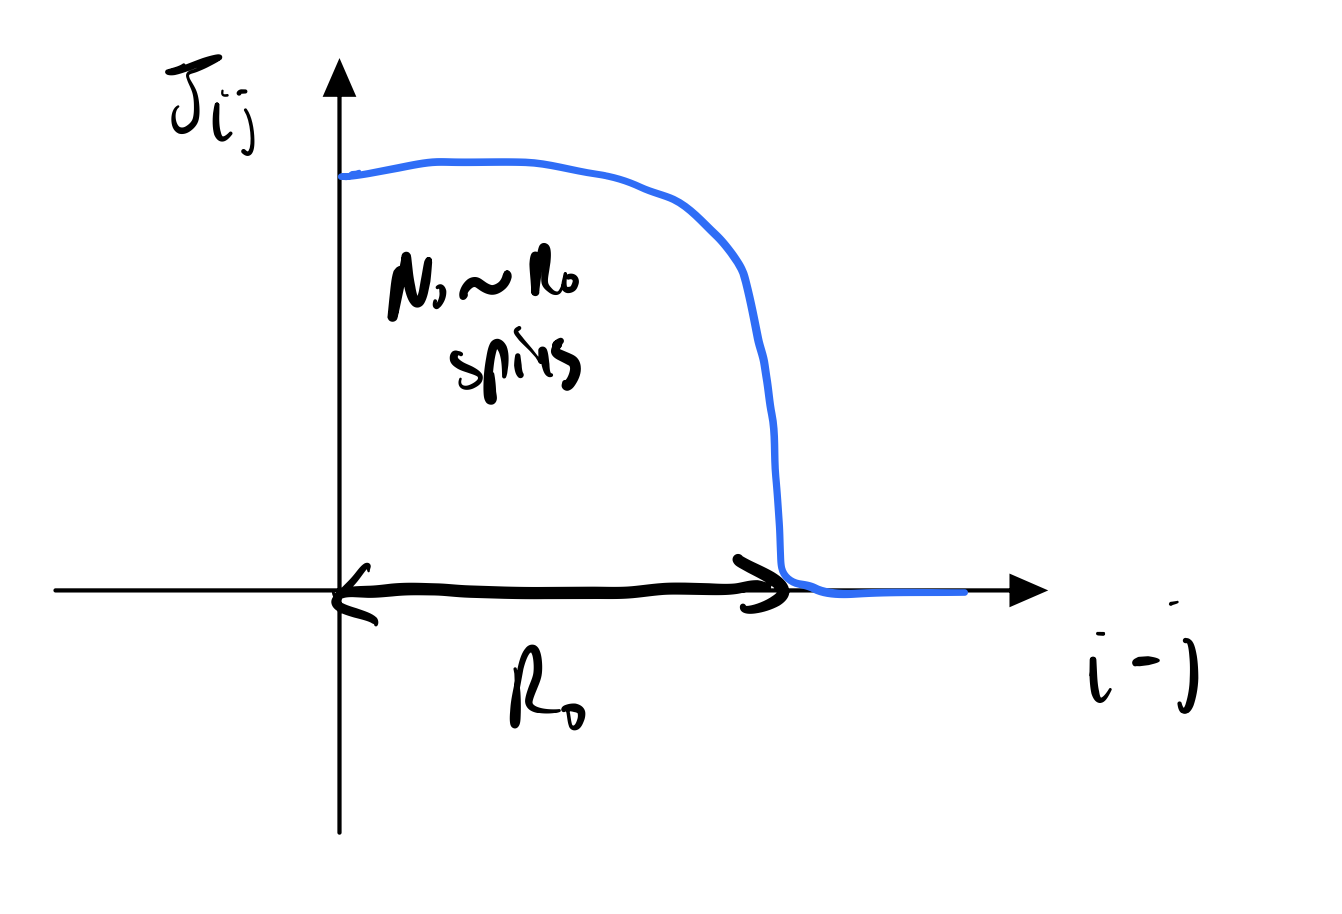
\includegraphics[scale=0.5]{Lectures/Figures/finite_range_interactions.png}
    \caption{Plot of the interactions/couplings $J_{ij}$, where the interactions are the same up to some long length scale $R_0$.}
    \label{fig:finite_range_interactions}
\end{figure}

In the Ising model, this looks like:
\begin{equation}
    H = \sum_{ij}JS_iS_j = \frac{J}{N_0}\sum_{\abs{i-j} < R_0}S_iS_j
\end{equation}
This looks like a coarse grained version:
\begin{equation}
    H = \sum_i S_i h_i
\end{equation}
where:
\begin{equation}
    h_i = \frac{J_0}{N_0}\sum_i S_i = J_0\avg{S}
\end{equation}
In the $N_0 \to \infty$ limit, this theory becomes correct (i.e. long range interactions get us closer to mean field theory, which makes sense! If all spins interact with each other, then the mean field literally is the physical field felt). A variant of this was used to win the Nobel prize last week (We will discuss the Hopfield model later in the course - it is a ferromagnet).

Note that the saddle point approximation works in a high number of dimensions, but it generally fails in a small number of dimensions - despite the dominance of the saddle point, there are many ways of making fluctuations; hence entropy comes in, competing with the energetics argument we have made here.

\subsection{Fluctuations}
We have two classes of models we consider, characterized by their symmetries.

\subsubsection*{Continuous (Rotational) Symmetries}
These are found, e.g., in X-Y models, Heisenberg models, superconductors. These generically have symmetries like $U(1), O(2), SO(2)$. The order parameters have amplitude and a phase, $\psi(x) = \abs{\psi_0}e^{i\theta(x)}$. At the mean field level, we can write $\abs{\nabla m}^2 = m_0^2 \abs{\nabla \Theta}^2$. We consider Hamiltonians with fluctuations of the form:
\begin{equation}
    \beta H = \text{Const} + \int d^d x\{\frac{1}{2}k\abs{\nabla\psi}^2\} \to \abs{\psi_0}^2\int d^dx \frac{1}{2}k(\nabla \Theta)^2 
\end{equation}
The stiffness is $\frac{1}{2}k\abs{\psi_0}^2$, where $\psi_0$ is the order parameter. Because this vanishes above the transition, the modes do not have stiffness above the critical point; they do below, with the stiffness vanishing as they approach the critical temperature. We can rewrite this as:
\begin{equation}
    \frac{1}{2}\abs{\psi_0}^2k\sum_a a \abs{\Theta_a}^2
\end{equation}
If we start populating these modes (as if they are bosons), we can get a very large number of them. We saw this in the AFM spin chain. Something similar will happen here. 

Why are they called soft modes? If I am far below $T_c$, the slope inb the dispersion relation is finite. As I approach $T_c$ in the mean field model, the slope goes to zero as the order parameters go to zero. Hence, they are ``soft''.

\begin{figure}[htbp]
    \centering
    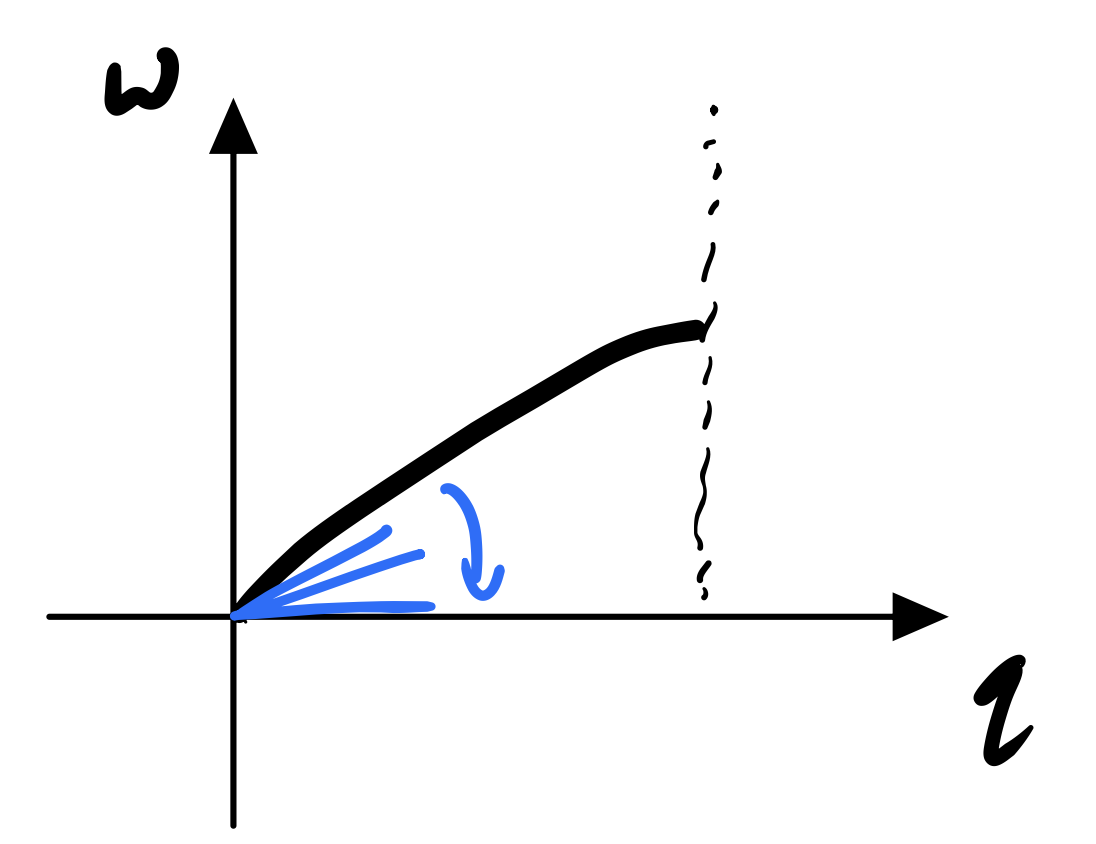
\includegraphics[scale=0.4]{Lectures/Figures/soft_modes.png}
    \caption{Depiction of ``soft modes'' in the dispersion relation, where as the temperature approaches the critical temperature below the slope in the dispersion (and the ``stiffness'') approaches zero.}
    \label{fig:soft_modes}
\end{figure}

\subsubsection*{Discrete ($\ZZ_2$) symmetry}
Next, we consider;
\begin{equation}
    \beta H = \int d^dx[\phi = \frac{1}{2}tm^2 + \frac{1}{4}um^4 + \frac{1}{2}k(\nabla m)^2]
\end{equation}
To which we can consider a more general E-L equation to find the extremum:
\begin{equation}
    k\nabla^2 m = tm + um^3
\end{equation}
We can now consider solutions that start into one well and cross into another well. We can solve this explicitly:
\begin{equation}
    m = m_0\tanh(\frac{x-x_0}{\omega})
\end{equation}
where the width is:
\begin{equation}
    \omega = \sqrt{\frac{2k}{-t}}
\end{equation}
This is another stationary solution; we previously found the lowest energy solution, this is a higher-lying stationary solution. As $t \to 0$, the domain wall becomes very long and the energy goes to zero. Notably, this is a particle-like excitation, with a lot of degrees of freedom as there are many points where it could be placed. Thus, we have to sum over all possible places to put 1, 2, \dots, $N$ domain walls. Each one has finite/small energy, but there are very many of these, so the entropic contribution is likely to win.

Next class, we will discuss how to measure these fluctuations (i.e. scattering experiments).
\section{Fluctuations, Continued}

\subsection{Phase and Amplitude Fluctuations}
We consider $\phi$ (the effective Hamiltonian/energy):
\begin{equation}
    \phi(\v{m}) = \frac{\kappa}{2}\abs{(\nabla \v{m})}^2 + \frac{t}{2}m^2 + \frac{u}{4}m^4
\end{equation}
where $\v{m}$ is a order parameter with magnitude $m = \abs{\v{m}(\v{x})}$ but also a phase (as it has a direction).

Looking at the potential, we have massless ``Goldstone'' modes that go between the two wells and the massive modes that oscillate inside of a given well.

\begin{figure}[htbp]
    \centering
    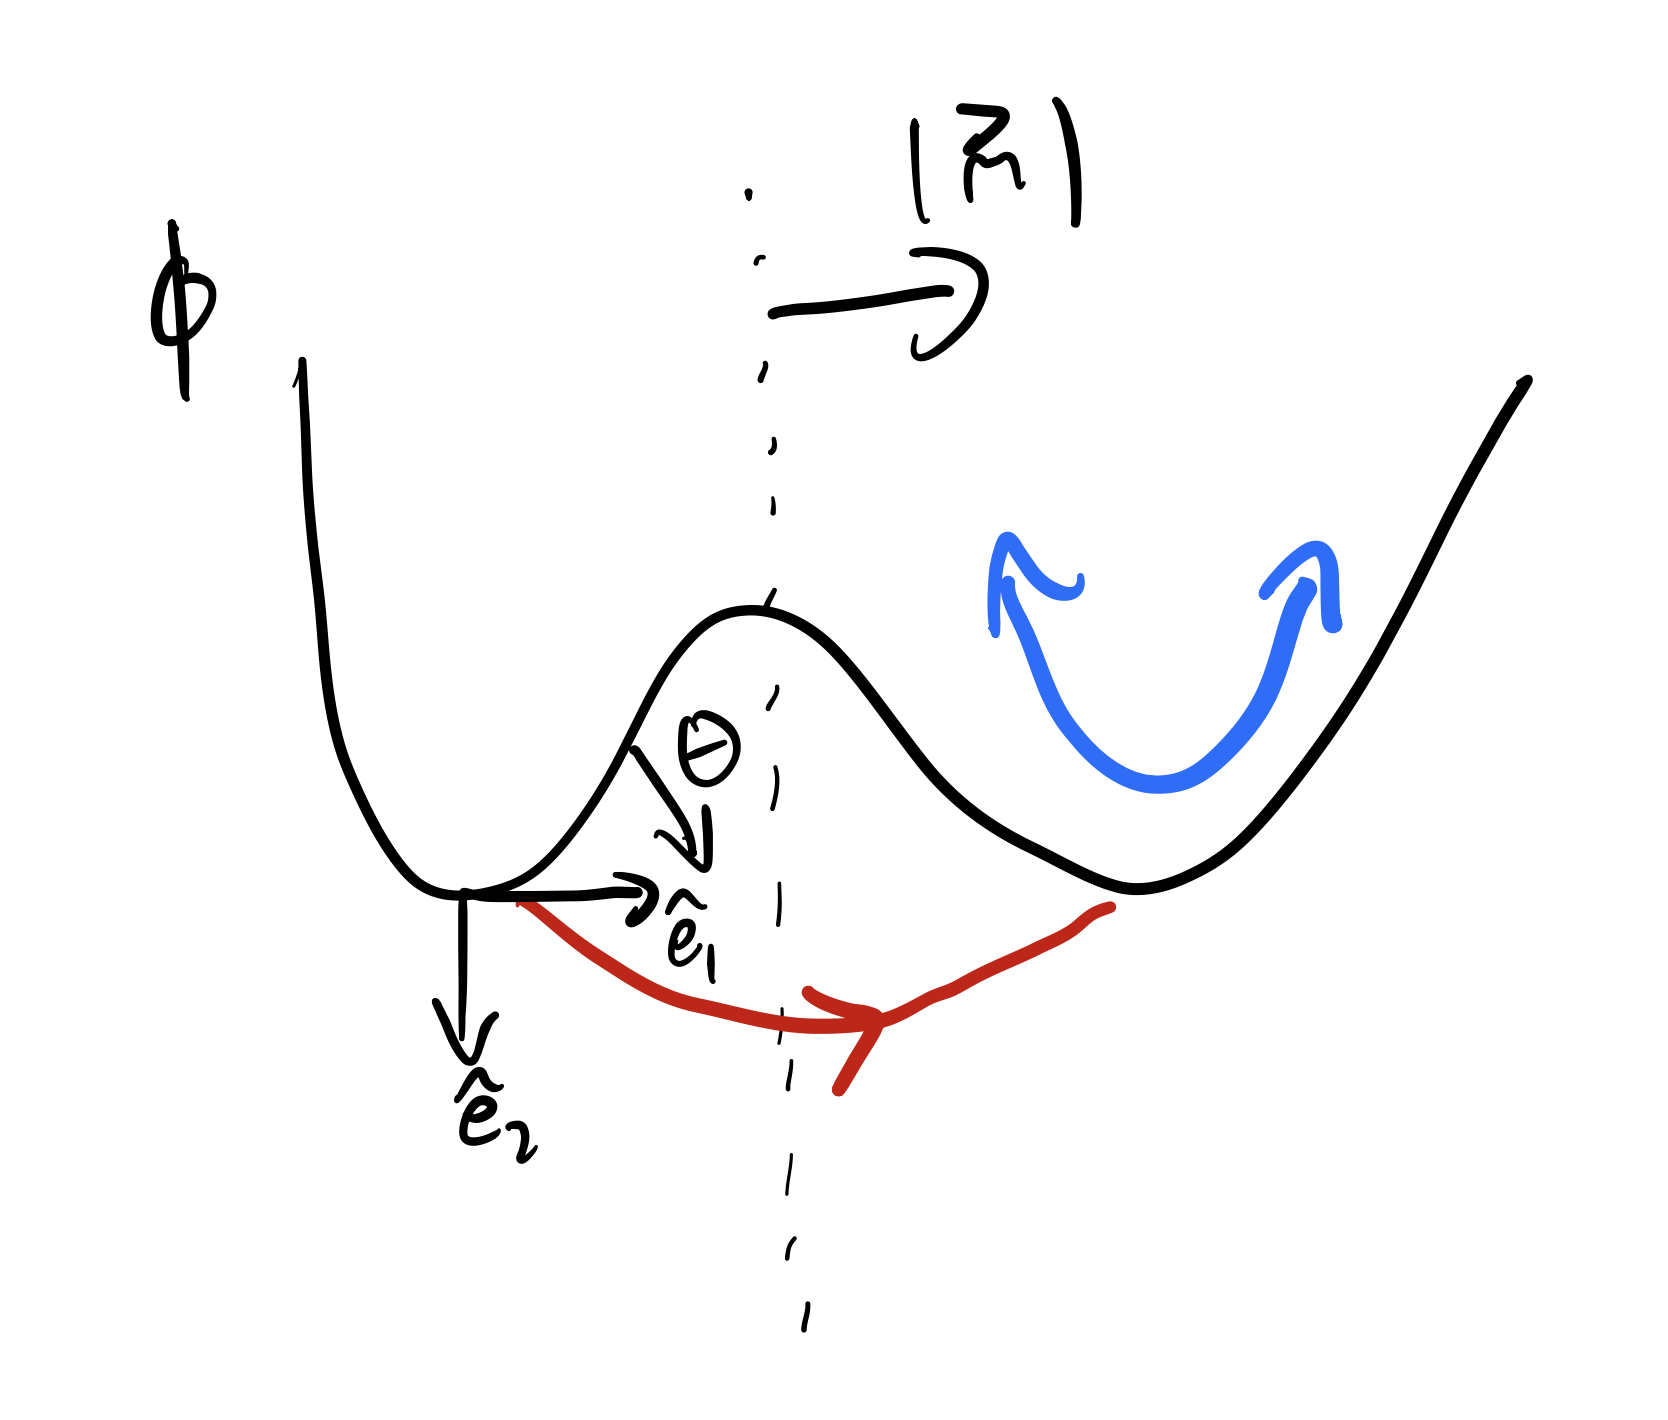
\includegraphics[scale=0.3]{Lectures/Figures/mexican_hat_fluctuations.png}
    \caption{We consider a potential/energy $\phi$ that depends on an order parameter $\v{m}(\v{x})$. The order parameter has magnitude $m = \abs{\v{m}}$ and direction $\theta$. There are massless Goldstone modes (red) that go between the wells of the potential, and massive modes that stay within a potential. For a given direction of the order parameter, we choose locally a coordinate system such that $\hat{e}_1$ points along the direction of magnetization and $\hat{e}_2$ (and other vectors) to be mutually orthogonal. This plot is for $t < 0$.}
    \label{fig:mexican_hat_fluctuations}
\end{figure}

We wish to find the probability distribution:
\begin{equation}
    \mathcal{P}[\v{m}(\v{x})] = \exp(-\int d^dx \phi(\v{m}, \v{x})).
\end{equation}

Let us notate $\avg{m} = \bar{m}$ and then write:
\begin{equation}
    m = [\bar{m} + \phi_l(\v{x})]\hat{e}_1 + \sum_{\alpha=2}^n \phi_{t, \alpha}(\v{x})\hat{e}_\alpha
\end{equation}
Where $\hat{e}_1$ is a vector parallel to the magnetization, and and $\hat{e}_\alpha$ for $\alpha = \set{2, \ldots, n}$ are vectors perpendicular to the magnetization and mutually orthogonal. The $\phi_l, \phi_t$ appearing above are the longitudinal and transverse fluctuations, respectively.

We consider the mean field solution:
\begin{equation}
    \bar{m} = \begin{cases}
    0 & t > 0
    \\ \sqrt{-\frac{t}{u}} & t < 0
    \end{cases}
\end{equation}
Which we then obtain:
\begin{equation}
    -\ln \mathcal{P} = V\left[\frac{t}{2}\bar{m}^2 + \frac{u}{4}\bar{m}^4\right] + \int d^dx \left(\frac{\kappa}{2}\abs{\nabla \phi_l}^2 + \left(\frac{t + 3u\bar{m}^2}{2}\right)\phi_l^2\right) + \int d^dx \left(\frac{\kappa}{2}\abs{\nabla \phi_t}^2 + \left(\frac{t + u\bar{m}^2}{2}\right)\phi_t^2\right) + O(\phi_{l/t}^4)
\end{equation}
Let us rescale:
\begin{subequations}
    \begin{align}
        \frac{\kappa}{\xi_l^2} &= t + 3u\bar{m}^2 = \begin{cases}
            t & t > 0
            \\ -2t & t < 0
        \end{cases}
        \\ \frac{\kappa}{\xi_t^2} &= t + u\bar{m}^2 = \begin{cases}
            t & t > 0
            \\ 0 & t < 0
        \end{cases}
    \end{align}
\end{subequations}
Where the $\xi$ are called correlation lengths. Above the mean-field phase transition they are the same. Below, they are different. The $0$ is the Goldstone mode (gapless, linear) and the $-2t$ is the massive mode (gapped, looks like a harmonic oscillator at long wavelengths).

We now have translation invariance, so a natural change of basis is to go into Fourier/momentum space:
\begin{equation}
    \phi(x) = \sum_\v{q} \phi_\v{q} \frac{e^{i\v{q} \cdot \v{x}}}{\sqrt{V}}
\end{equation}
We then find:
\begin{equation}
    \mathcal{P}[\phi_{l\v{q}}, \phi_{t\v{q}}] \propto \prod_{\v{q}, \alpha}\exp(-\frac{\kappa}{2}\left(\v{q}^2 + \xi_\alpha^{-2}\right)\abs{\phi_{\alpha\v{q}}}^2)
\end{equation}
We can now start to compute objects of interest, e.g. correlation functions (between fluctuations). We call this the structure factor:
\begin{equation}\label{eq:structurefactor}
    S(\v{q}) = \avg{\phi_{\alpha\v{q}}\phi_{\beta\v{q}'}} = \frac{\delta_{\alpha\beta}\delta_{\v{q},-\v{q}'}}{\kappa(q^2 + \xi^2_\alpha)}
\end{equation}
The decoupling of longitudinal/transverse gives the first delta function and the second comes from momentum conservation. The denominator comes from the computation of the Gaussian integrals. Plotted, it looks like:

\begin{figure}[htbp]
    \centering
    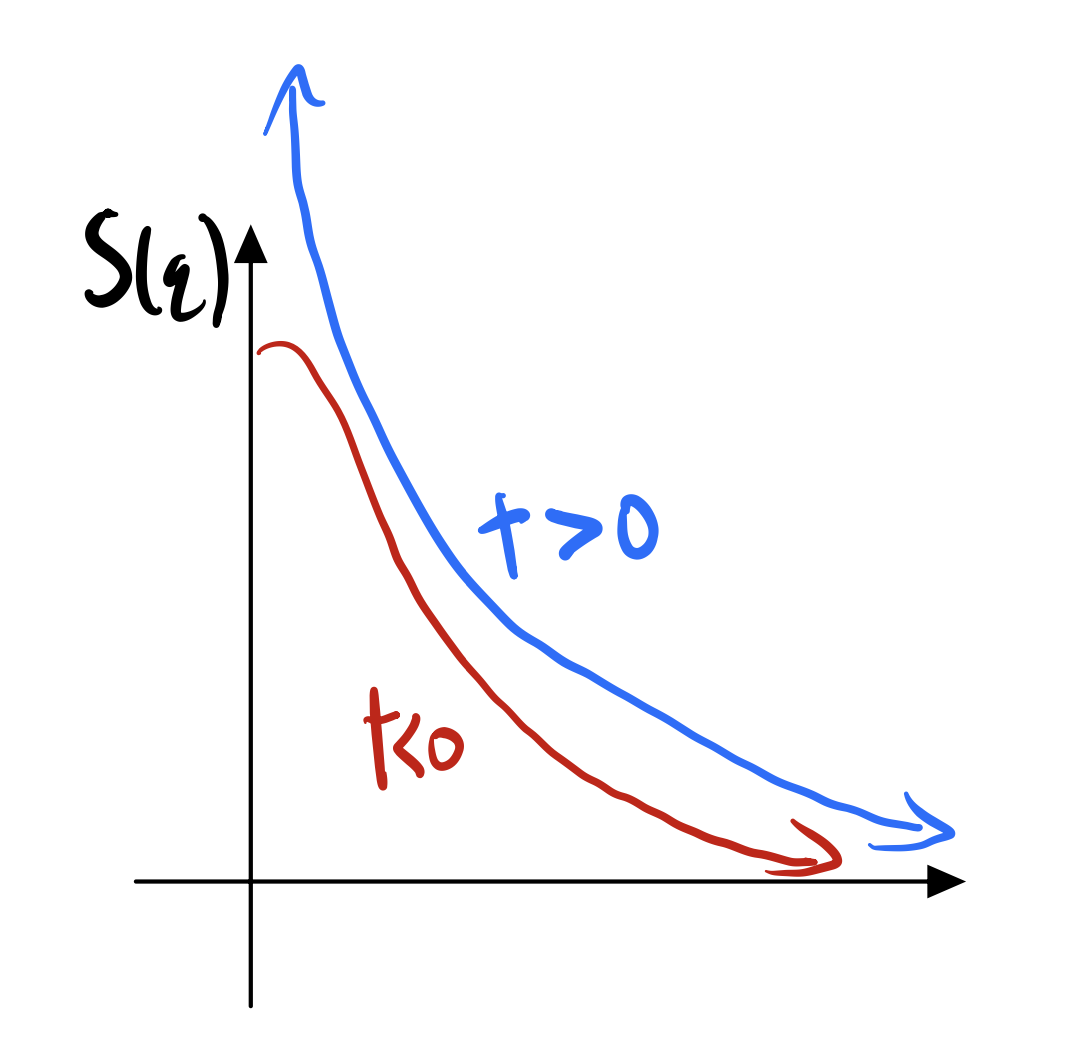
\includegraphics[scale=0.3]{Lectures/Figures/structure_factor.png}
    \caption{Plot of structure for transverse modes as a function of $q$. For $t < 0$ we have $\xi_t = 0$ and so the structure factor diverges at $0$. For $t > 0$, $\xi_t$ is finite so the structure factor at $0$ does not diverge. The structure factor for the longitudinal fluctuations has the same general shape as the $t > 0$ transverse fluctuations (for $t < 0$ and $t > 0$; $\xi_l$ is finite for both regimes, just with a different prefactor. For $t > 0$ it is identical to the transverse fluctuations).}
    \label{fig:structure_factors}
\end{figure}

What is the interpretation of $S(\v{q})$? We have some object of interest, which we probe via a scattering experiment. We have some probe, which could be an electron, neutron, photon etc. It has an incident wavevector $\v{k}_i$ and a output wavevector $\v{k}_f$, emerging at some angle $\theta$ to the incident. If we have elastic scattering, then the energy of the particle remains unchanged, but there is some changed momenta, i.e. $\v{k}_f = \v{k}_i + \v{q}$. We then study the scattering amplitude:
\begin{equation}
    A(q) \propto \bra{\v{k}_f}\v{U}\ket{\v{k}_i} \propto \sigma(\v{q})\int d^dx e^{i\v{q}\cdot \v{x}}\rho(\v{x}) \propto \rho_\v{q}
\end{equation}
Note that the average over the scattering amplitude vanishes:
\begin{equation}
    \avg{A(q)} = \avg{\rho_\v{q}} = 0
\end{equation}
So to probe the structure we want to study:
\begin{equation}
    S(q) = \avg{\abs{A(\v{q})}^2} \propto \avg{\rho_\v{q}}
\end{equation}

\subsection{Technical Aside: Gaussian Integrals}
Consider the single variable integral:
\begin{equation}
    I_1 = \int_{-\infty}^\infty d\phi e^{-\frac{1}{2}k\phi^2 + n\phi}
\end{equation}
We solve via completing the square and then redefinition of the integration variable to $\phi' = \sqrt{k}(\phi - \frac{h}{k})$. What is left with just the familiar Gaussian integral, which we should be familiar with the result of:
\begin{equation}
    I_1 = \int_{-\infty}^\infty d\phi e^{-\frac{1}{2}k(\phi - \frac{h}{k})^2 + \frac{h^2}{k}} = \sqrt{\frac{2\pi}{k}}e^{\frac{h^2}{2k}}
\end{equation}
Now consider $\dod{I_1}{h}$, which via differentiating under the integral sign we know is equivalent to $\avg{\phi}$.
\begin{equation}
    \dod{I_1}{h} = \int d\phi \phi e^{-(\ldots)} = \avg{\phi} = \frac{h}{k}
\end{equation}
This integral is correct up to a constant factor. We don't have to care about these constants, as eventually we take the logarithm of the partition function, and this becomes an additive constant which has no effect on the physics. We can also look at the second derivative:
\begin{equation}
    \dod[2]{I_1}{h} = \avg{\phi^2} = \frac{h}{k} + \frac{h^2}{k^2}
\end{equation}
We can also look at the cumulant:
\begin{equation}
    \avg{\phi^2}_c = \avg{\phi^2} - \avg{\phi}^2 = \frac{h}{k}.
\end{equation}
In principle we could go to higher order cumulants, but you can verify for yourself that these would all vanish.

Now, let's look at the $N$-dimensional version:
\begin{equation}
    I_N = \int_{-\infty}^\infty \prod_{i=1}^N d\phi_i \exp(-\frac{1}{2}\sum_{ij}\phi_i K_{ij}\phi_j + \sum_i n_i \phi_i) = \sqrt{\frac{(2\pi)^N}{\det K}}\exp(\sum_{ij}h_i \frac{K_{ij}^{-1}}{2}h_j)
\end{equation}
How would we obtain this? $K$ is a general, presumably symmetric matrix. We diagonalize $K$, and suppose it has eigenvalues $K_{ij}\hat{q}_j = K_q \hat{q}_j$. We use the $\hat{q}_j$ as the canonical basis, and rotate into this basis by saying $\phi_i = \sum_q \tilde{\phi}_q \hat{q}_i$. Thus the integral becomes:
\begin{equation}
    I_N = \int \prod_{q=1}^N d\tilde{\phi}_q \exp(-\frac{K_q}{2}\phi_q^2 + h_q\tilde{\phi}_q) = \prod_{q=1}^N\sqrt{\frac{2\pi}{K_q}}\exp(h_q\frac{K_q^{-1}}{2}h_q)
\end{equation}
where now recognizing the determinant is just the product of the eigenvalues, and rotating back into the eigenbasis, gives the desired expression.

Remark: This relation is very useful, and it works out for QFTs as well, with some $i$s floating around.

\subsection{Back to Physics - Transverse Fluctuations and Coloumb Emergence}
Now, we make the remark that all Gaussian theories are \emph{solvable} - they may be wrong, but they are solvable. In other words, mean field theory + fluctuations to lowest order (i.e. quadratic) are completely solvable analytically, and are known as Gaussian theories. They are simple, but already can give us interesting phenomena.

For example, for the structure factors appearing in Eq. \eqref{eq:structurefactor}, we were able to find this just with a Gaussian theory, and it tells us that the long wavelength/small $q$ is the interesting regime where things are happening. We can look at the exponent $\eta$ that tells us how the structure factor scales.
\begin{equation}
    S(q, t=0) \sim \frac{1}{q^{2 - \eta}}
\end{equation}

Let us focus on the tranverse fluctuations, below the critical temperature, so $t < 0$ with $\eta_t = 0$. Then, we have:
\begin{equation}
    \mathcal{P}(\Theta(q)) \propto \exp(-\frac{\kappa}{2}\sum_q q^2\abs{\Theta_q}^2)
\end{equation}
So with out computed structure factor, let us look at the probability fluctuations in the angles:
\begin{equation}
    \avg{\Theta_\v{q}\Theta_{\v{q}'}} = \frac{\delta_{\v{q} + \v{q}'}}{\kappa q^2}
\end{equation}
Going back into real space, this is the statement that:
\begin{equation}
    \avg{\Theta(\v{x})\Theta(\v{x}')} = \frac{1}{V}\sum_\v{q}e^{i\v{q}(\v{x} - \v{x}')}{\kappa q^2} = \int \frac{d^dq}{(2\pi)^d}\frac{e^{i\v{q}\cdot(\v{x} - \v{x}')}}{q^2}
\end{equation}
This is just the Coloumb potential:
\begin{equation}
    C(\v{x}) = -\int \frac{d^d q}{(2\pi)^d}\frac{e^{i\v{q}\cdot\v{x}}}{q^2}
\end{equation}
Which satisfies $\nabla^2 C = \delta^d(\v{x})$, i.e. just Gauss' Law for a point charge. Now, we can ask what happens to the potential as $x \to \infty$?
\begin{equation}
    \lim_{x \to \infty}C(x) \propto \begin{cases}
        \text{Const} & d > 0
        \\ x^{2-d} & d < 2
        \\ \ln(x) & d =2 
    \end{cases}
\end{equation}
This behaviour can be obtained by looking at $d^dq \sim q^{d-1}dq$ (plus various angular integrals which we don't care about). 

Thus, in low dimensions the correlations fall off like a power law, so no long range order. For $d > 2$ we maybe have LRO. At $d = 2$, we have the critical/marginal dimension. We have a pesky logarithm, and we need more work (which we will study in future lectures).

Earlier on, we explained how there were models (AFM Heisenberg) that did not order at low dimensions due to the presence of soft modes. This is a souped up version of that. So, when generally looking at a theory, if I look at a theory with Goldstone modes, I should look at the phase fluctuations and see if I get LRO. Even though in principle the length scales can get very large, we can still say that at very large scales that the correlations fall off. Also, its worth noting that the LRO is temperature dependent; we dropped the $\beta$s through the calculations here, but it is relevant.
\section{Scaling Theory}
\subsection{Recap}
To recap; we are studying Gaussian theory, in particular $\phi^4$ theory of a magnet. This is mean field theory + quadratic fluctuations, which is exactly solvable, but can still give us insight.

We looked at correlation length associated to longitudinal and transverse fluctuations. We studied the effect of the transverse fluctuations/Goldstone mode, and below 2-$d$ the correlations die off and we have no LRO. This was the lower critical dimension. We will now study an upper critical dimension, which will turn out to be $d = 4$.

We look at the logarithm of the partition function:
\begin{equation}
    \ln Z = \frac{t}{2}\bar{m}^2 + \frac{u}{4}\bar{m}^4 + \int d^dx \left[\frac{1}{2}\kappa(\nabla \phi_l)^2 + \xi_l^{-2} \phi_l^2\right] + \int d^dx \left[\frac{1}{2}\kappa(\nabla \phi_t)^2 + \xi_t^{-2}\phi_t^2\right]
\end{equation}
The correlation lengths have the scaling:
\begin{equation}
    \xi_l = \begin{cases}
        \xi_0 t^{-1/2}  & t > 0 
        \\ (-2t)^{-1/2} & t < 0
    \end{cases}
\end{equation}
\begin{equation}
    \xi_t = \begin{cases}
        \xi_0 t^{-1/2} & t > 0 
        \\ \infty & t < 0
    \end{cases}
\end{equation}
The important observation for the transverse modes is below the phase transition, the $\xi_t\phi_t^2$ term is absent. We can do the integral by going into momentum space:
\begin{equation}
    \int d^dx \left[\frac{1}{2}\kappa(\nabla \phi_t)^2 + \xi_t^2\phi_t^2\right] = \int \frac{d^dq}{(2\pi)^d} \left[\frac{1}{2}\kappa (q^2 + \xi_t^{-2})\phi_t(q)^2\right]
\end{equation}
Then the partition function is:
\begin{equation}
    Z = Z_{MF}e^{-\ln\det(\kappa(q^2 + \xi_t^{-2}))}
\end{equation}
Where this comes from:
\begin{equation}
    Z = \int \mathcal{D}\phi_q e^{-\frac{1}{2}\int d^d q\kappa (q^2 + \xi_t^{-2})\phi_q^2}
\end{equation}
And then we take the Gaussian integral. Then computing the correlators from this result (dropping $\xi_t$ as we are $t < 0$);
\begin{equation}
    \avg{\phi_t(\v{q}), \phi_t(\v{q}')} = \frac{\delta_{\v{q} + \v{q}'}}{\kappa \v{q}^2} \implies \avg{\phi_t(\v{x})\phi_t(\v{x}')} = \int \frac{d^dq}{(2\pi)^d} \frac{e^{i\v{q} \cdot \v{x} - \v{x}'}}{\kappa \v{q}^2}
\end{equation}
from which we saw that:
\begin{equation}
    \lim_{x \to \infty}C(x = \abs{\v{x} - \v{x}'}) \propto \begin{cases}
        \text{Const} & d > 0
        \\ x^{2-d} & d < 2
        \\ \ln(x) & d =2 
    \end{cases}
\end{equation}
and found our lower critical dimension of $2$. 

\subsection{Massive Modes and Upper Critical Dimension}
We have the partition function of the longtitudinal modes:
\begin{equation}
    Z = Z_{MF}e^{-\ln\det(\kappa(q^2 + \xi_l^{-2}))}
\end{equation}
Let us look at the free energy, by taking the logarithm of $Z$:
\begin{equation}
    F = F_{MF} + \frac{1}{2}\int \frac{d^dq}{(2\pi)^d} \ln(\kappa(\v{q}^2 + t))
\end{equation}
Now looking at the heat capacity:
\begin{equation}
    C = -T\dpd[2]{F}{T} \sim -t\dpd[2]{F}{t}
\end{equation}
Looking at the contribution from the fluctuations:
\begin{equation}
    C \sim \int \frac{d^dq}{(2\pi)^d}\frac{1}{(\kappa q + t)^2} \stackrel{t \to 0}{\sim} \int_0^{1/a} dq \frac{q^{d-1}}{q^4} \sim a^{4d}
\end{equation}
we want to see how this integral behaves. For $d > 4$, we have the integral is well behaved at $q = 0$ and evaluates to $\sim a^{4d}$ as above. For $d < 4$, we need to keep the correlation length (else the integral does not converge) so:
\begin{equation}
    \int_0^{1/a}dq \frac{q^{d-1}}{(q^2 + \xi_l^{-2})} \sim \xi^{4-d}
\end{equation}
Plotting the heat capacity, we get:

\begin{figure}[htbp]
    \centering
    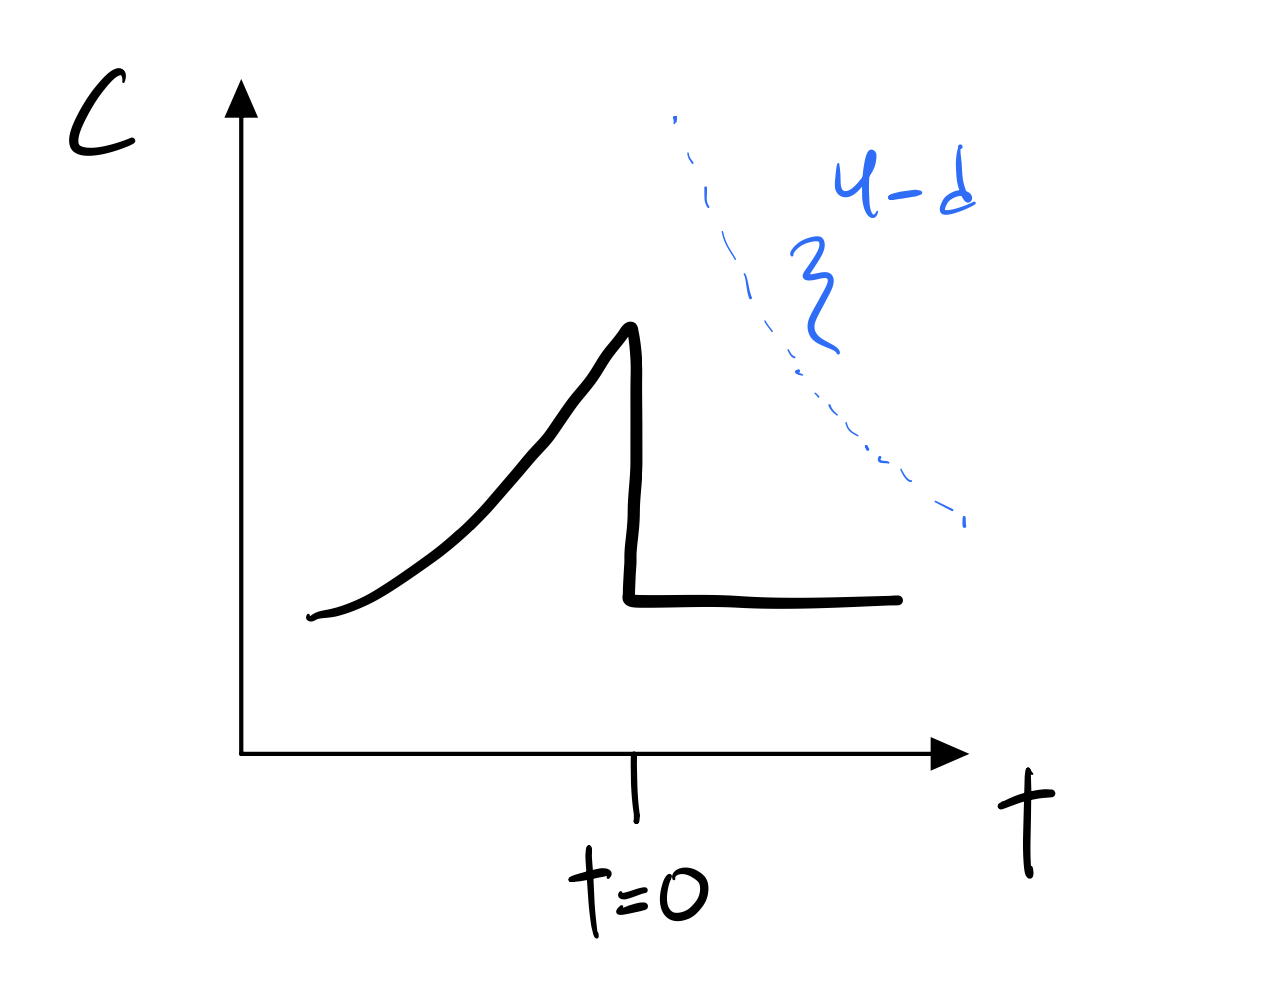
\includegraphics[scale=0.5]{Lectures/Figures/lec6heatcapacity.png}
    \caption{Plot of heat capacity for Gaussian theory.}
    \label{gaussian-heatcapacity}
\end{figure}

So, we see that Gaussian theory fails for $d < 4$. Why? We said MF theory + small fluctuations. If the effect of small fluctuations is benign, then we are happy. If the effect of small fluctuations is large, then we aren't happy; the theory is not self-consistent. Below $d < 4$, the failure of the integral to converge (and the rapid change in behaviour of physical quantities due to the fluctuations) tells us that the theory does not apply.

So below $d = 2$ we have no LRO, and above $d = 4$ we know that MFT + Gaussian fluctuations is ok. The interesting regime left to explore is $d = 2$ to $d = 4$. 

We also were studying the phase transition at $t = 0$ we can also ask about the magnitude of the fluctuations as we go away from the transitions.

In summary, we saw that the heat capacity from the mean field goes as $C_{MF} = \frac{1}{u}$ and the capacity of the fluctuations go as $C_{F} = \frac{\xi^{4-d}}{\kappa^2}$. The $\kappa$ is a microscopic parameter that characterizes the stiffness of the bare mode, with dimensional analysis from $\kappa \nabla^2$ telling us that $\kappa$ has a dimension of length square, i.e. $\kappa \sim \xi_0^{2}$. Thus:
\begin{equation}
    C_F \sim \frac{\xi_0^{4-d}\abs{t}^{-\frac{4-d}{2}}}{\xi_0^4} = \frac{1}{\xi_0^d}t^{-\frac{4-d}{2}}
\end{equation}
so indeed the $t$ piece diverges, but we have the $\xi_0$ piece characterizing the microscopic correlation length. So, if we have a system with a very long microscopic correlation length, we have to get very close to the transition $t = 0$ to see the divergence. This defines a temperature where the fluctuations where the fluctuations take over and the theory fails. This temperature is typically known as the \emph{Ginzburg temperature}. There are systems, typically superconductors, where the microscopic correlation length is very long. So, despite the fact that the correlations diverge, we have to get very close to the transitions to see these diverging correlations.

\subsection{Scaling Theory}
Is it going to be the case where I need a theory that calculates a new parameter for each fluctuating quantity? Or are they all related? Our proposal is the latter. Let us make this statements precise

\emph{Scaling theory:} Thermodynamic functions (e.g. the thermodynamic free energy $F$) are homogenous functions of scaled variables (e.g. $T, h$).

This hypothesis can be used to simplify the problem such that I may compute simple things. To be clear, we already had this in mean field theory. There, we looked at some (scaled) free energy which we viewed as the minimum of a power series expansion:
\begin{equation}
    f(t, h) = \min_m \left[\frac{t}{2}m^2 + \frac{u}{4}m^4 - hm\right]
\end{equation}
For example, this gave:
\begin{equation}
    f(t, h) = \begin{cases}
        -\frac{t^2}{4u} & h = 0, t < 0
        \\ -\frac{3}{4}\frac{h^{4/3}}{u^{1/3}} & h \neq 0, t = 0
    \end{cases}
\end{equation}
With a crossover line $h \sim \abs{t}^{3/2}$ below which we have the first behaviour, and above which we have the second.

\begin{figure}[htbp]
    \centering
    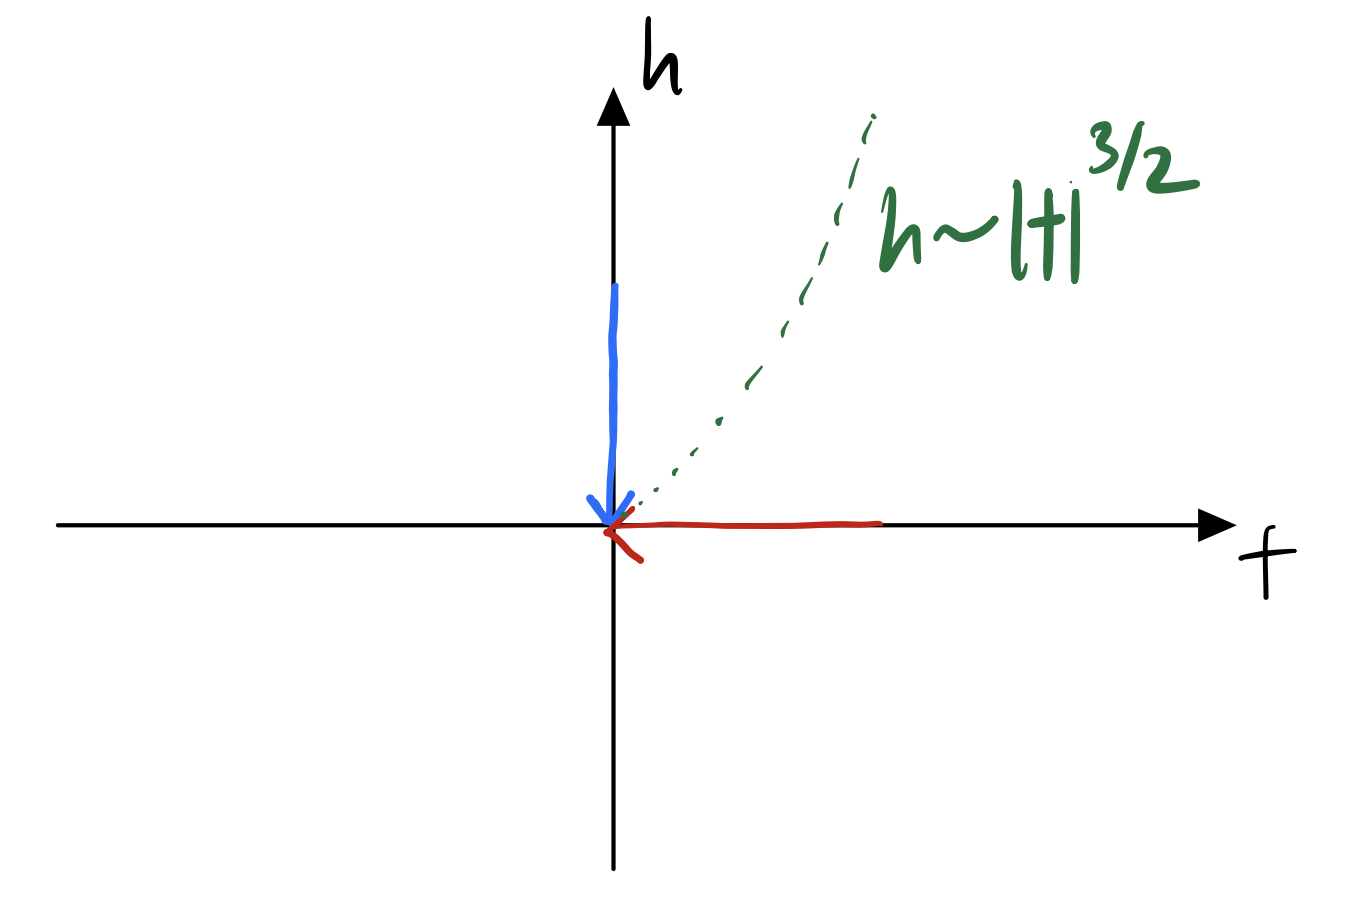
\includegraphics[scale=0.5]{Lectures/Figures/htcrossover.png}
    \caption{The free energy has a certain behaviour aloing the $h = 0$ and $t = 0$ lines. The crossover of these two behaviours occurs along $h \sim \abs{t}^{3/2}$.}
    \label{fig-htcrossover}
\end{figure}

Rewriting this in another way, We have:
\begin{equation}
    f(t, h) = \abs{t}^2g(h/\abs{t}^\Delta)
\end{equation}
where $g$ is a homogenous function of $h/\abs{t}^\Delta$. The previous calculations constrain $g$. E.g. at $g = 0$, we have:
\begin{equation}
    g(0) = -\frac{1}{4u}
\end{equation}
and
\begin{equation}
    g(x\to\infty) \sim x^{4/3}
\end{equation}
In the limit where $h$ is large, we also know the answer is independent of $t$, therefore if we have:
\begin{equation}
    f(t, h) = \abs{t}^2\left(\frac{h}{\abs{t}^\Delta}\right)^{4/3}
\end{equation}
the $t$-independence constrains $\Delta = 3/2$. 

In MF theory, we know precisely what $g$ is. In general with scaling analysis, we only know the asymptotic behaviour.

What we will do - we propose that there is a ``better theory'', where:
\begin{equation}
    f_{\text{sing}}(t, h) = \abs{t}^{2-\alpha}g(h/\abs{t}^\Delta)
\end{equation}
The singular component to the energy goes as:
\begin{equation}
    \begin{split}
        E_{\text{sing}} \sim \dpd{f}{t} &= (2-\alpha)\abs{t}^{1-\alpha}g(h/\abs{t}^\Delta) - \Delta h \abs{t}^{1-\alpha-\Delta}g'(h/\abs{t}^\Delta)
        \\ &= \abs{t}^{1-\alpha}\left((2-\alpha)g(h/\abs{t}^\Delta) - \Delta(\frac{h}{\abs{t}^\Delta})g'(h/\abs{t}^\Delta)\right)
    \end{split}
\end{equation}
where the term in brackets is another homogenous function, $g_E(h/\abs{t}^\Delta)$. To get the heat capacity, we take the derivative again:
\begin{equation}
    C_{\text{sing}} \sim -\dpd[2]{f}{t} = \abs{t}^{-\alpha}g_c(h/\abs{t}^\Delta)
\end{equation}
and we have the magnetization:
\begin{equation}
    m(t, h) = \dpd{f}{h} = \abs{t}^{2-\alpha-\Delta}g_m(h/\abs{t}^\Delta)
\end{equation}
now, as $h \to 0$, we have $g_m \to \text{const}$, and we identify the critical exponent $\beta = 2 - \alpha - \Delta$. For large arguments, we propose $g_M(x) \sim x^P$, then:
\begin{equation}
    m(t=0, h) \sim \abs{t}^{2-\alpha-\Delta}\left(\frac{h}{\abs{t}^\Delta}\right)^P
\end{equation} 
so by the $t$-independence argument, we have:
\begin{equation}
    2 - \alpha - \Delta = P\Delta
\end{equation}
and then:
\begin{equation}
    m(h) \sim h^{\frac{2-\alpha-\Delta}{\Delta}}
\end{equation}
so then we identify the exponent:
\begin{equation}
    \delta = \frac{\Delta}{2 - \alpha - \Delta} = \frac{\Delta}{\beta}
\end{equation}
whose measurement allows us to infer $\Delta$.

Why might this theory be true? Underlying this theory is a diverging correlation length, which gives you averaging, and is solely responsible for the singular fluctuations. The last thing we propose is that there is a correlation length $\xi$ that is hidden behind all of this phenomenology, where:
\begin{equation}
    \xi \sim \abs{t}^{-\nu}g_\xi(\frac{h}{\abs{t}^\Delta})
\end{equation}
where the divergence of $\xi$ is responsible for the rest of the behaviour we have analyzed. 

This is the hypothesis, and we have to work out this hypothesis in such a way that is self-consistently well behaved. The process we will go through (known as the \emph{renormalizaiton group}) will start with a Ginzburg-Landau theory, suggest there is a diverging length scale that is responsible for the phenomena, and then average that action on a characteristic length scale. We then scale. Then, supposing that the correlation length gets scaled, we can average again, and we want to force the averaging procedure to give us a function which is a homogenous function of the parameters. This is the process/constraint we put on scaling. We force the algebra to give us a scaling function like this. When we do this, there is a sequence of operations that will enable us to calculate these exponents. We can then check if the procedure is consistent, or not. This is what we will explore in future lectures.C
\section{Scaling Hypothesis Part II and Renormalization Group}
\subsection{Recap}
We postulate a free energy:
\begin{equation}
    f_{\text{sing}}(t, h) = \abs{t}^{2-\alpha}g(h/\abs{t}^\Delta)
\end{equation}
where the exponents are different from those appearing in mean field theory, and $g$ is a homogenous function of its argument. From this, we are able to derive for a scaling law for the magnetization $m$, for the specific heat $C$, the susceptibility $\chi$, etc.

If this holds, we have a correlation length:
\begin{equation}
    \xi(t, h) = \abs{t}^{-\nu}g_\xi(h/\abs{t}^\Delta).
\end{equation}
In MF theory, $\nu = 1/2$, but it may be different here. We will find $\mu > 0$ so the correlation length diverges as $T \to T_c$.

We assume that $\ln Z$ is extensive, i.e. $\propto L^d$ (it is very rare that this would not be the case). More specifically, $\ln Z \propto \frac{L^d}{\xi^d}$ plus any nonsingular terms. Then the free energy goes as:
\begin{equation}\label{eq:singfreeenergy}
    f_{\text{sing}} = \frac{\ln Z}{L^d}g(h/\abs{t}^\Delta) \propto \abs{t}^{d\nu}g(\cdot)
\end{equation}
which implies:
\begin{equation}
    2-\alpha = d\nu
\end{equation}
This is known as the hyperscaling, or Josephson relation. It doesn't work in MF theory, unless $d = 4$. In one of the homework problems, we will muse on why this is.

We study the correlation function:
\begin{equation}
    G(\gamma, 0) = \avg{m(\gamma)m(0)} - \avg{m}^2 \sim \frac{1}{\abs{\gamma}^{d-2+\eta}}
\end{equation}

\begin{figure}[htbp]
    \centering
    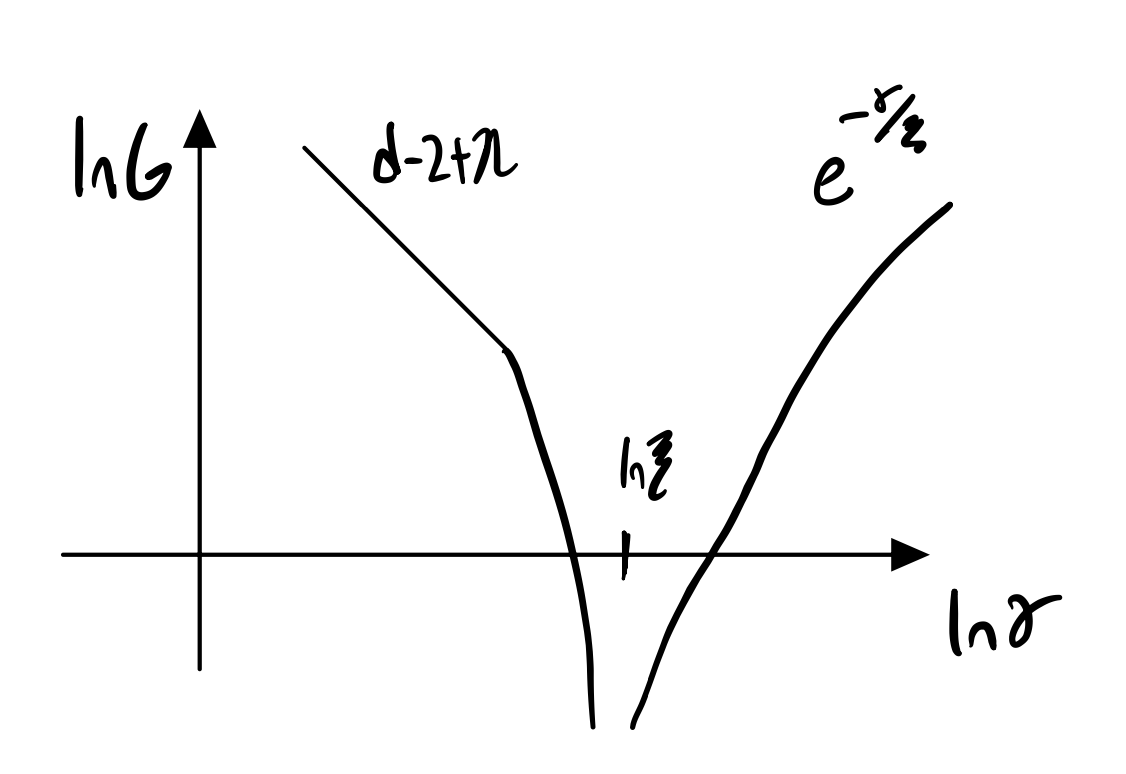
\includegraphics[scale=0.5]{Lectures/Figures/correlation_scaling.png}
    \caption{At long distances, the correlation functions die off exponentially. Near the critical point, it is a power law.}
    \label{fig:correlation_scaling}
\end{figure}

We now study the renormalization group, which allows us to mathematically obtain these exponents. We start with a conceptual view.

\subsection{Renormalization Group: Conceptual View}
\subsubsection*{Step 1: Coarse Graining}
We do RG via a process of coarse graining. We take a length scale $x$, and convert it to $bx$ where $b > 1$. Pictorially, we look at a $bx \times bx$ block of spins and average them to form an ``averaged spin'' corresponding to that whole block. I.e. the magnetization as a function of $x$ becomes:
\begin{equation}
    m(x) = \frac{1}{b^d}\int d^dx' m(x')
\end{equation}
where we integrate over the cell center at $x$.

\begin{figure}[htbp]
    \centering
    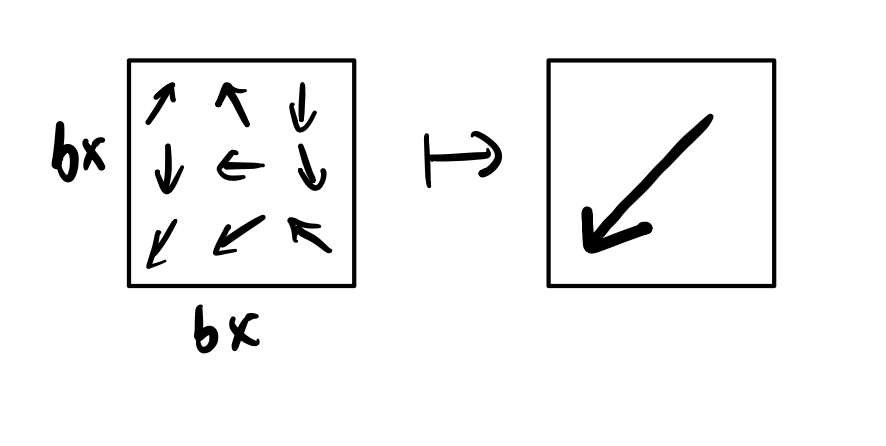
\includegraphics[scale=0.5]{Lectures/Figures/blockspins.png}
    \caption{At the coarse graining step, we integrate over a block of spins and replace it with the average.}
    \label{fig:blockspins}
\end{figure}

Notice that we lose information when we do this. Via course graining, we lose the microscopics.

\subsubsection*{Step 2: Rescale}
We now take $x_{\text{new}} = \frac{x_{\text{old}}}{b}$, rescaling/blowing up the new cell size to be the size of the original unit cell.

\subsubsection*{Step 3: Renormalize}
We renormalize the magnetization:
\begin{equation}
    m_{\text{new}}(x_{\text{new}}) = \frac{1}{\xi b^d}\int d^dx'm(x')
\end{equation}
Where to make the theory look the same as when we started, we introduce a new renormalization parameter $\xi$.

\subsection{Getting Exponents out of RG}

Having done this, we can construct a new probability distribution:
\begin{equation}
    W[m_{\text{new}}] = e^{-\beta H_b[m_{\text{new}}]}
\end{equation}

We will assert that at criticality ($t = h = 0$), the Hamiltonian is statistically similar to the one I had originally. This means of course that in this theory, we introduce a new effective temperature and field that must be a function of the old ones. I.e.:
\begin{equation}
    \begin{split}
        t_{\text{new}} &= f(t_{\text{old}}, h_{\text{old}})
        \\ h_{\text{new}} &= f'(t_{\text{old}}, h_{\text{old}})
    \end{split}
\end{equation}
but we have some constraints. $(0, 0) \to (0, 0)$, and $t_{\text{new}}, h_{\text{new}}$ should grow. Since we rescale the length, the correlation length should get shorter, so we grow away from the $0$ point. We also hope that there is no singular behaviour in these functions. Finally, we want to preserve the symmetry; as such, we will not mix $t$ with $h$. Then:
\begin{equation}
    \begin{split}
        t_b(t, h) &= A(b)t + O(t^2)
        \\ h_b(t, h) &= B(b)h + O(h^2)
    \end{split}
\end{equation}
We know that:
\begin{equation}
    A(1) = B(1) = 1
\end{equation}
(This corresponds to no scaling). There is also the assumption that this could be repeated:
\begin{equation}
    t_{b_1b_2}(t, h) = A(b_1b_2)t = A(b_1)A(b_2)t
\end{equation}
In other words, scaling once by $b_1b_2$ should be the same as scaling by $b_2$ and then $b_1$. This implies that:
\begin{equation}
    A(b) \sim b^{y_t} \quad B(b) \sim b^{y_h}
\end{equation}
Notice that this is a semigroup, as we can only go one way. So, this isn't actually a group (Renormalization group is a bit of a misnomer). This is how we can see the ``loss in information'' of this process.

We also assume that $y_t, y_h > 0$. So, we go further from the critical point. This might cause us concern because then the higher order $t^2, h^2$ terms in the scaling may become relevant. But indeed we take $b \sim 1$ in order to stay within a neighbourhood of the critical point, as this is the only regime in which this analysis is actually valid. Then, looking at the the scaling of the general functions:
\begin{equation}
    X(t, h) = b^{y_x}X(b^{y_t}t, b^{y_h}h)
\end{equation}
and the new configuration becomes:
\begin{equation}
    Z = \int \mathcal{D}mW[m]
\end{equation}
but the weights of the old configuration should be the same as the old one, so:
\begin{equation}
    Z = \int \mathcal{D}mW[m] = \int \mathcal{D}m' W[m'] = Z'
\end{equation}
Which then leads us to conclude that:
\begin{equation}
    Vf(t, h) = V'f(t',h')
\end{equation}
So then looking at the scaling of the free energy:
\begin{equation}
    f(t, h) \sim \frac{1}{b^d}f(b^{y_t}t, b^{y_h}h)
\end{equation}
We now have to propose a trajectory to scale such that we eventually get to the form $\abs{t}^{2-\alpha}g(h/\abs{t}^\Delta)$. We take $b^{y_t}t \sim 1$ so $b\sim t^{-1/y_t}$. Then:
\begin{equation}
    f(t, h) = \frac{1}{b^d}f(1, h/t^{y_h/y_t})
\end{equation}
So, we are taking the free energy, positing a scaling form, and we get out something that looks like Eq. \eqref{eq:singfreeenergy} as we desired.

From this, we obtain:
\begin{equation}
    2 - \alpha = \frac{d}{y_t}
\end{equation}
\begin{equation}
    \Delta = \frac{y_h}{y_t}
\end{equation}
What we will do is find a scaling path and determine the scaling exponents $y_h, y_t$, and then this tells us about the critical exponents of our interest. Let's look at the others.

There will now be a new correlation length:
\begin{equation}
    \chi' = \chi/b
\end{equation}
Looking at the general form of the scaling of the correlation length:
\begin{equation}
    \chi(t, h)= b\chi(b^{y_t}t, b^{y_h}h) = t^{-1/y_t}\xi(1, h/t^{y_h/y_t}) 
\end{equation}
and thus:
\begin{equation}
    \nu = -\frac{1}{y_t} = \frac{2-\alpha}{d}
\end{equation}
which is the Josephson scaling relation.

Let us look at the magnetization as well"
\begin{equation}
    m(t, h) = \frac{1}{V}\dpd{\ln Z}{h} = b^{y_h - d}m(1, h/t^{y_h/y_t})
\end{equation}
so then:
\begin{equation}
    \beta = \frac{d}{y_t} - \frac{y_h}{y_t} = 2-\alpha-\Delta
\end{equation}

\subsection{RG Fixed Points and Flows}
To start, we write down the most general Hamiltonian allowed by symmetry. For example here:
\begin{equation}
    \beta H = \int d^d x\left[\frac{1}{2}tm^2 + \frac{1}{4}um^4 + \frac{1}{6}vm^6 + \frac{1}{2}K(\nabla m)^2 + \frac{1}{2}L(\nabla^2 m)^2 + \ldots\right]
\end{equation}
I now have a parameter space $S(t, u,  v, K, L, \ldots)$ in which the parameters define a point.

Then, we'll go through the RG process. We course grain by averaging over block size $b$, rescale $x \to x/b$, then normalize by $\xi$. We then have the magnetization:
\begin{equation}
    m'(x') = \frac{1}{\xi b^d}\int d^dxm(x)
\end{equation}
We then construct $P[m']$ from $P[m]$ (nontrivial process!). We then get a rescaled Hamiltonian $H'(t', u', v', K', L', \ldots)$. This process is the same as saying that:
\begin{equation}
    S' = R_b S
\end{equation}
i.e. we have applied a map to our parameter space.

We consider a deviation:
\begin{equation}
    S^*_\alpha + \delta S_\alpha' = S_\alpha^* + (R_b)_{\alpha\beta}\delta S'_\beta
\end{equation}
where $S^*$ is the fixed point of the RG theory (imagine we have done the calculation and found this point/the critical point), i.e.:
\begin{equation}
    R_bS^* = S^*
\end{equation}
and $\xi(S^*) = b\xi(R_b S^*)$ i.e. $\xi \to \infty$. We can write the renormalization group map (the $L$ denoting the linearized version of the map, which we assume we can do in the vicinity of the critical point) as:
\begin{equation}
   (R^L_b)_{\alpha\beta} = \dpd{S'_\alpha}{S_\beta}
\end{equation}
i.e. the RG takes us from $S_\alpha$ to $S'_\alpha$. Now, consider this map to have eigenvectors $\Theta_i$ and eigenvalues $\lambda(b)_i$. Then:
\begin{equation}
    R_b^L R_{b'}^L\Theta_i = \lambda_i(n)\lambda_i(b') = \lambda_i(b'b').
\end{equation}
thus:
\begin{equation}
    \lambda_i(b) \sim b^{y_i}
\end{equation}
Therein, the $\Theta_i$ correspond to scaling directions and the $y_i$ correspond to anomalous dimensions (in MF theory they are all 1 - not anomalous). We now expand $S$ around the fixed point based on these scaling directions:
\begin{equation}
    S = S^* + \sum_i g_i \Theta_i
\end{equation}
After we scale:
\begin{equation}
    S' = S^* + \sum_i g_i b^{y_i}[\Theta]
\end{equation}
Pictorally, we have the flows in Fig. \ref{fig:RGflows}.

\begin{figure}[htbp]
    \centering
    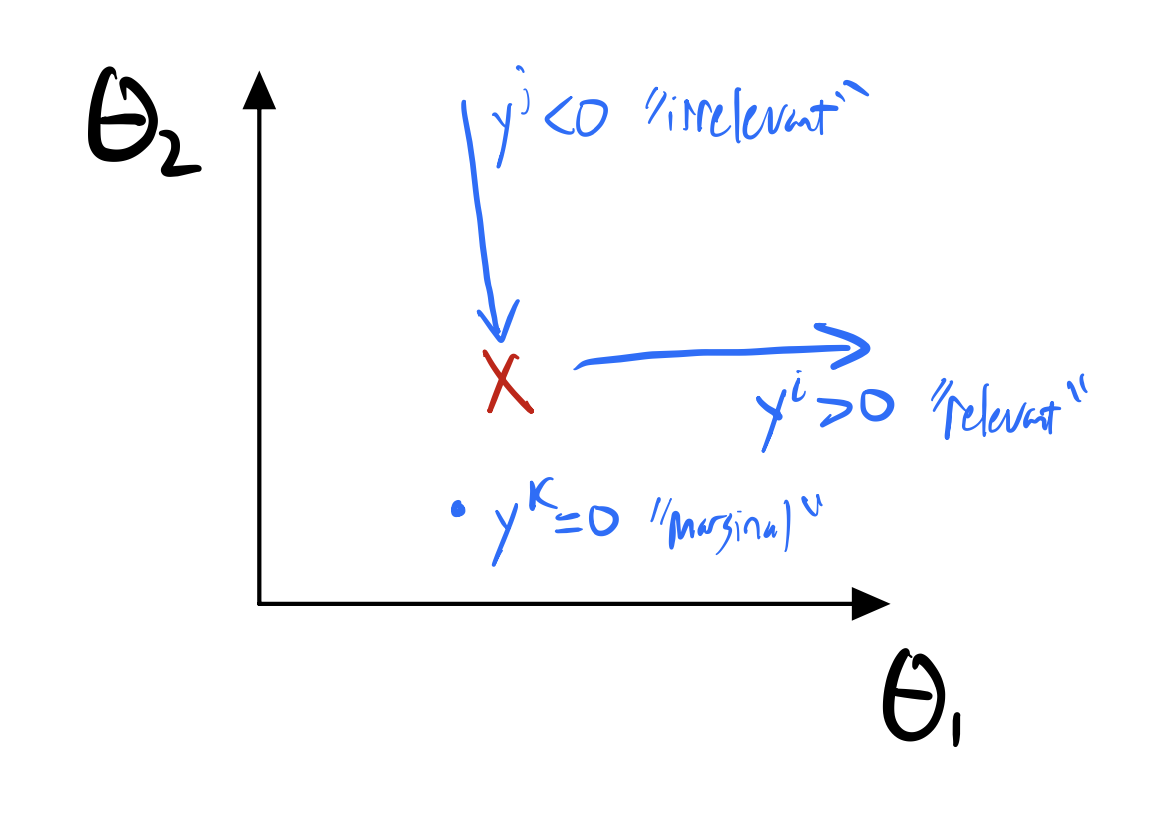
\includegraphics[scale=0.5]{Lectures/Figures/RGflows.png}
    \caption{Different eigenvectors have different flow properties. Irrelevant eigenvectors go towards the fixed point, relevant eigenvectors flow away, and marginal eigenvectors are stationary.}
    \label{fig:RGflows}
\end{figure}

The vectors define a basin of attraction. Relevant means the eigenvectors go away from the fixed point, so the fluctuations grow and become important. Irrelevant mean the eigenvectors go towards the fixed point, so the fluctuations vanish (hence irrelevant). Finally, we have $y_i = 0$ and then we call the flows ``marginal''. These directions correspond to some linear combinations to linear combinations of the parameters $t, u, v, K, L,\ldots$ of the theory. The main takeaway is that this flow analysis tells us what variables are the important ones.

Next Wednesday, we will go through this process for the Gaussian theory, and identify the Wilson-Fisher fixed point.
\section{Renormalization Group Part II}
Today, we will go through the RG procedure on a model which is exactly solvable. 

\subsection{Exact Solution of Gaussian Model}
Consider the following partition function for a Gaussian model:
\begin{equation}
    Z = \int \mathcal{D}m(x)\exp\left(-\int d^dx \left(\frac{1}{2}tm^2 + \frac{1}{2}k(\nabla m)^2 + \frac{1}{2}L(\nabla^2 m)^2 - mh\right)\right)
\end{equation}
We go into momentum space:
\begin{equation}
    m(\v{q}) = \int d^dx e^{i\v{q} \cdot \v{x}}m(\v{x})
\end{equation}
Then:
\begin{equation}
    m(\v{x}) = \sum_{\v{q}}\frac{e^{-i\v{q} \cdot \v{x}}}{V}m(\v{q}) = \int \frac{d^d q}{(2\pi)^d}m(\v{q})
\end{equation}
Note the factor of volume to ensure the average magnetization does not scale with the size of the system. We then have:
\begin{equation}
    \beta H = \sum_{\v{q}}\left(\left[\frac{t + kq^2 + Lq^4}{V}\right]m(q)^2 - hm(\v{q})\delta_{\v{q}0}\right)
\end{equation}
Then:
\begin{equation}
    Z = \prod_{\v{q}}\left(\frac{1}{\sqrt{V}}\right)^n \int dm\v{q} \exp\left(-\left(\frac{t + kq^2 + Lq^4}{V}\right)\abs{m(q)}^2 + hm(\v{q})\delta_{\v{q}0}\right)
\end{equation}
with $n$ the number of components. Then, factoring out the $\v{q} = 0$ term:
\begin{equation}
    Z_0 = \left(\frac{2\pi}{t}\right)^{n/2}\exp(\frac{Vh^2}{2t})
\end{equation}
And the rest of the partition function is:
\begin{equation}
    Z_{\text{rest}} = \prod_{q \neq 0}\left(\frac{2\pi}{t + kq^2 + Lq^4}\right)^{n/2}
\end{equation}
$Z$ is then:
\begin{equation}
    Z = \exp(\frac{Vh^2}{2t})\prod_{q\neq 0}\left(\frac{2\pi}{t + kq^2 + Lq^4}\right)^{n/2}
\end{equation}
Thus:
\begin{equation}
    F = -\frac{\ln Z}{V} = -\frac{h^2}{t} + n\int \frac{d^dq}{(2\pi)^q}\ln(t + kq^2 + Lq^4)
\end{equation}
What is the range of this integral? In general, we have a lattice, and we would integrate over a Brouillin zone. We approximate this region of integration as over a hypersphere with radius $\Lambda\sim \pi/a$:
\begin{equation}
    F = -\frac{h^2}{2t} + \frac{n\Omega_d}{2}\int_0^\Lambda dq q^{d-1}\ln(t + kq^2 + Lq^4)\Omega_d
\end{equation}
where $\Omega_d = S_d\frac{1}{(2\pi)^d}$ is the solid angle of a $d$-dimensional hypersphere. 

\begin{center}
    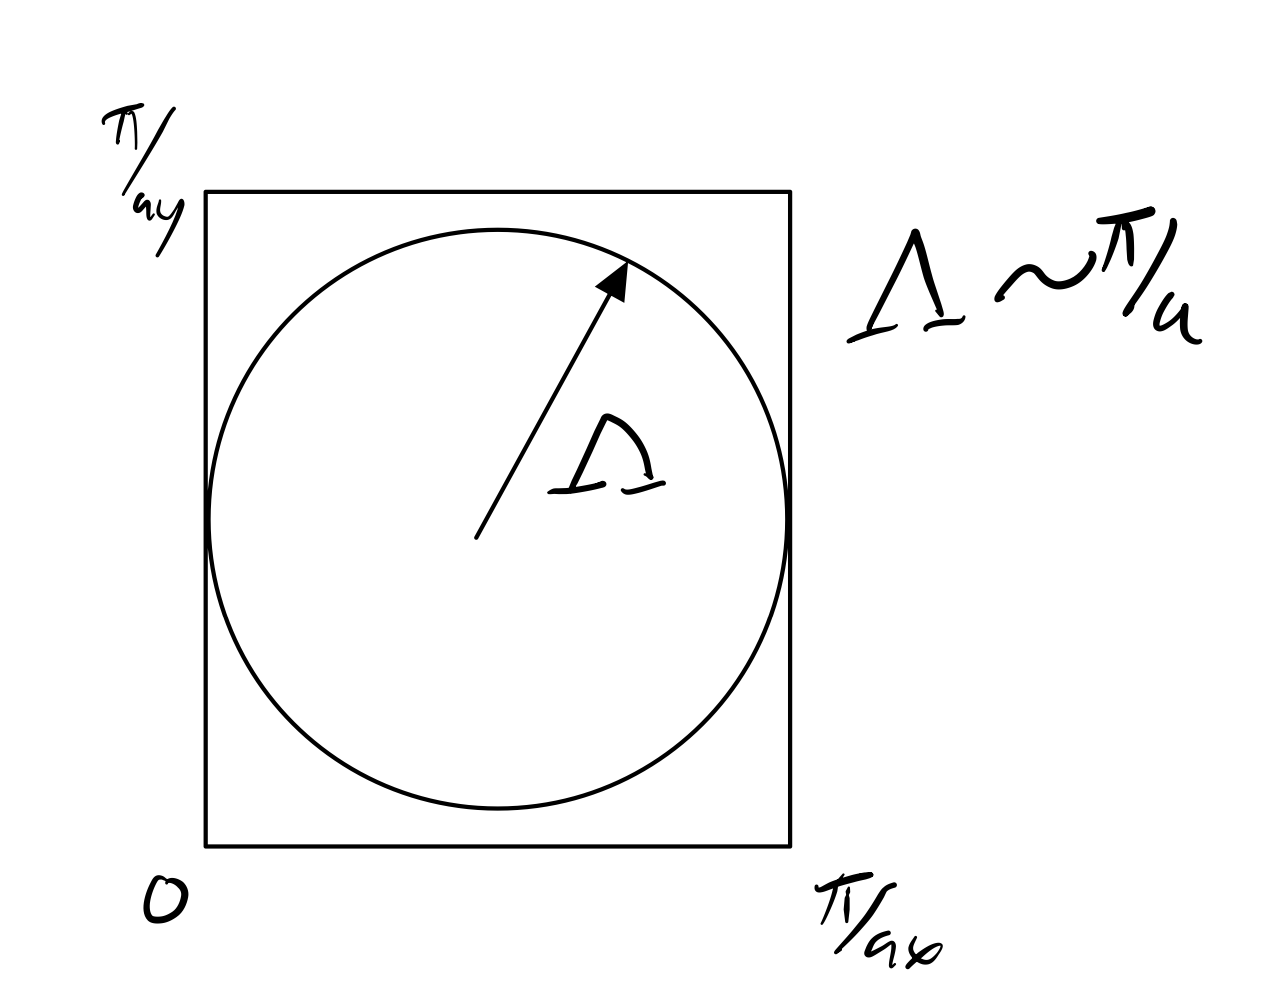
\includegraphics[scale=0.3]{Lectures/Figures/lec8-hypersphere.png}
\end{center}

We rescale the integral by defining $x = q/sqrt{t/k}$ which gives:
\begin{equation}
    F = -\frac{h^2}{2t} + \frac{n\Omega_d}{2}\left(\frac{t}{k}\right)^{d/2}\int_0^{\Lambda/\sqrt{t/k}} dx x^{d-1}\left(\ln t + \ln(1 + x^2 + \frac{Ltx^4}{k^2})\right)
\end{equation}
Note that if $t \ll 1$ the upper limit of the integral goes to infinity. Then we study the integral, and although it looks a little scary, it does turn out to converge. Note that in this limit, $L$ does not matter. It's a bit easier to compute the specific heat than the free energy directly. So, we can take two derivatives of $F$ and find $C$:
\begin{equation}
    C = -\dpd[2]{F}{T} = -n\frac{\Omega_d}{2}\left(\frac{t}{k}\right)^{d/2} \int_0^\infty dx \frac{x^{d-1}}{t^2(1 + x^2 + \frac{Lx^4t}{k^2})^2}
\end{equation} 
For $d > 4$ this is finite.

\subsection{RG approach to Gaussian model}
We return back to the partition function:
\begin{equation}
    Z = \int \mathcal{D}m(\v{q})\exp(-\int_0^\Lambda \frac{d^dq}{(2\pi)^d}\left[\left(\frac{t + kq^2 + Lq^4}{2}\right)\abs{m}^2 + hm(\v{q})\delta(\v{q})\right])
\end{equation}
\subsubsection*{Coarse Grain}
We consider $a < x < ba$ and then consider splitting the momentum space region into $0 < q < \Lambda/b$ and $\Lambda/b < q < \Lambda$, this latter region we call $\sigma(\v{q})$. 

\begin{center}
    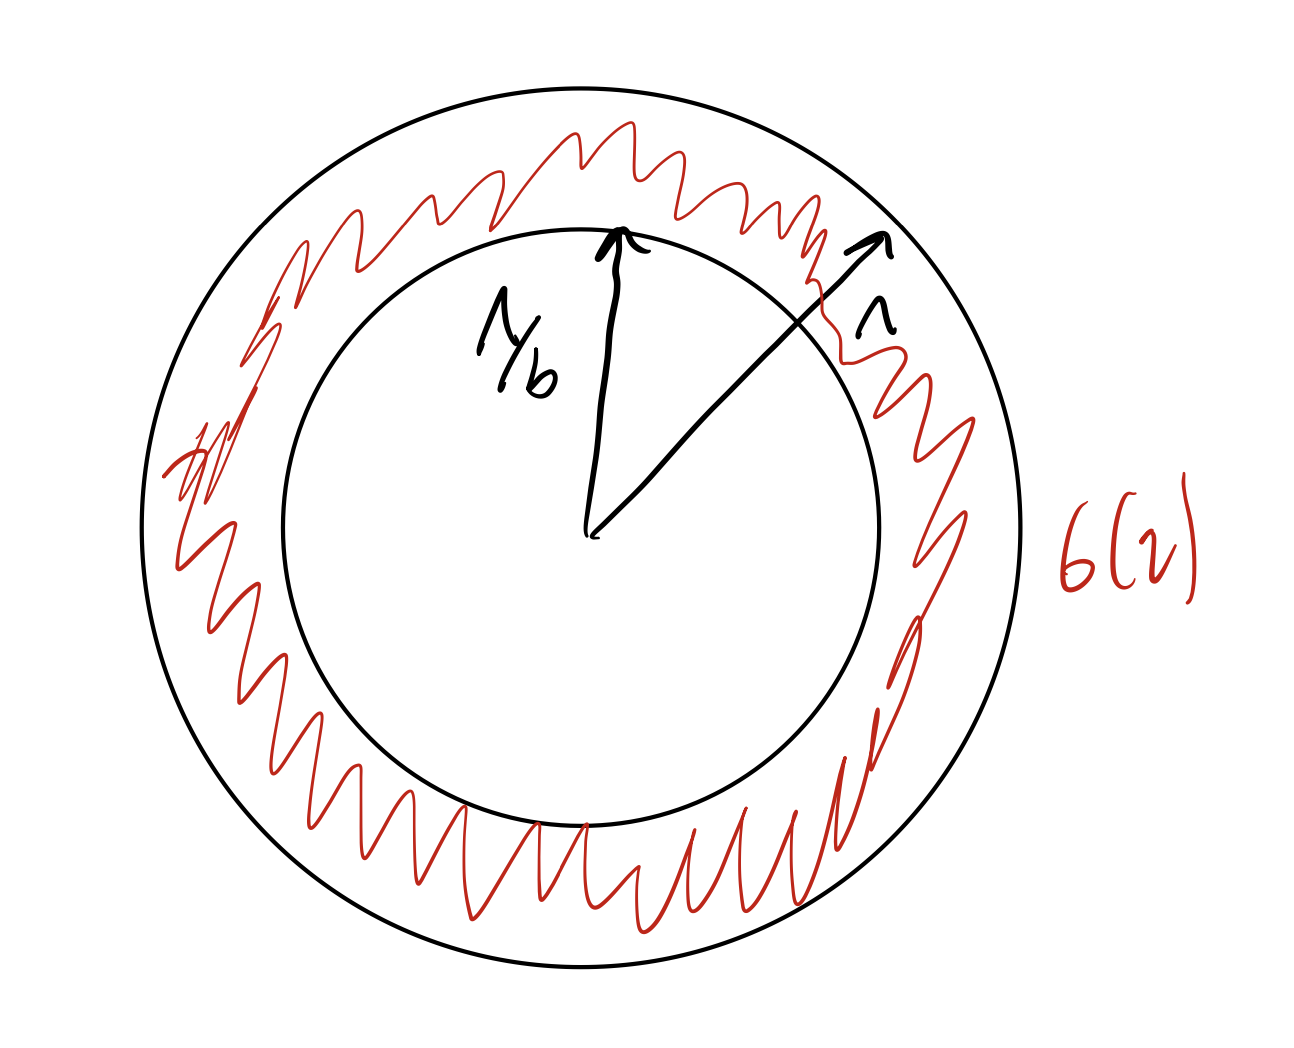
\includegraphics[scale=0.3]{Lectures/Figures/lec8-sphere-split.png}
\end{center}

We then split the integral into two parts:
\begin{equation}
    Z= \exp(-\frac{nV}{2}\int_{\Lambda/b}^\Lambda d^dq \ln(t + kq^2 + Lq^4)) \cdot \int \mathcal{D}m^<(\v{q})\exp(-\int_0^{\Lambda/b}\frac{d^dq}{(2\pi)^d}\left(t + kq^2 + Lq^4\right)\abs{m^<}^2 + hm^<(\v{q})\delta(\v{q}))
\end{equation}
where the first term corresponds to the result of doing the Gaussian integral over $\sigma(\v{q})$. Note we have called the dummy variable of integration $m^<$ to remind ourselves that these are the momenta $< \Lambda/b$ we have not yet integrated over.
\subsubsection*{Rescaling}
Call:
\begin{equation}
    \delta f_b(t) = \frac{n}{2}\int_{\Lambda/b}^\Lambda d^dq \ln(t + kq^2 + Lq^4)
\end{equation}
Now, we rescale $q' = bq$, then:
\begin{equation}
    Z = e^{-V\delta f_b(t)}\int \mathcal{D}m^<(\v{q}')\exp(-\int_0^\Lambda \frac{d^dq'}{(2\pi)^d}b^{-d}\left(\frac{t + kb^{-2}q^2 + Lb^{-4}q'^{4}}{2}\abs{m^<(\v{q}')}^2 + hm^<(\v{q}')\delta(\v{q'})\right))
\end{equation}
where the appropriate dimensional quantities have picked up factors from rescaling.

\subsubsection*{Renormalization}
We now renormalize:
\begin{equation}
    m'(q) = \frac{m^<(q)}{z}
\end{equation}
After we do this, the partition function now becomes:
\begin{equation}
    Z = e^{-V\delta f_b}\int \mathcal{D}m(\v{q})\exp(-\int_0^\Lambda \frac{d^dq}{(2\pi)^d}\left[b^{-d}z^2\left(\frac{t + kb^{-2}q^2 + Lb^{-4}q^4}{2}\right)\abs{m}^2 + zhm(\v{q})\delta(\v{q})\right])
\end{equation}
Nowm we rescale our parameters:
\begin{subequations}
    \begin{align}
        t_{\text{new}} &= z^2b^{-2}t 
        \\ h_{\text{new}} &= z h
        \\ k_{\text{new}} &= z^2b^{-d-2}k 
        \\ L_{new} &= z^2 b^{-d-4}L
    \end{align}
\end{subequations}
The $t = 0, h = 0$ singular point fortunately remain the same with the new parameters. If things are to be scale invariant at the singular/critical point, then $k_{\text{new}} = k$ (since we want the Hamiltonian to transform back to itself at the critical point - we take this as the definition) which enforces:
\begin{equation}
    z = b^{1 + d/2}
\end{equation}
So then:
\begin{equation}
    L_{\text{new}} = b^{-2}L
\end{equation}
so $L$ is irrelevant. (Note: We could not enforce $L_{\text{new}} = L$ and find a consistent set of equations, as if we did, we would find that $k$ would scale to $\infty$. We can propose fixed points, but if we propose $L$ as the leading order variable, then the other variables explode, so it is not a valid fixed point. The trivial scaling dimension of $k$ is $d + 2$ and for $L$ it is $d + 4$). We then find:
\begin{equation}
    t_{\text{neq}} = b^2t
\end{equation}
\begin{equation}
    h_{\text{neq}} = b^{1+d/2}h
\end{equation}
So then:
\begin{equation}
    y_t = 2
\end{equation}
\begin{equation}
    t_n = 1 + d/2
\end{equation}
Which gives us the critical exponents:
\begin{equation}
    \nu = 1/y_t = 1/2
\end{equation}
\begin{equation}
    \Delta = y_n/y_t = \frac{1}{2} + \frac{d}{4}
\end{equation}
\begin{equation}
    \alpha = 2-d\nu = 2 - d/2
\end{equation}
\begin{equation}
    \gamma = 1
\end{equation}
Our fixed point Hamiltonian (which is scale invariant) is:
\begin{equation}
    H^* = \frac{k}{2}\int d^dx \left(\nabla m \right)^2
\end{equation}
our results here agree with the exact solution obtained via solving the Gaussian theory. In the future, we will use the RG to solve problems that are not exactly solvable. But before we go to perturbative RG, a couple of technical points.

\subsection{Scaling dimension}
Consider:
\begin{equation}
    u_n\int d^d x m^n
\end{equation}
If we now find a fixed point and add a perturbation to the model, we can now power count after doing the RG:
\begin{equation}
    u_n\int d^d x m^n \to b^d z^n \int d^dx' m^n
\end{equation}
then, $u_n$ scales as:
\begin{equation}
    u_n' = u_n b^{d+n-nd/2} = u_n b^{y_n}
\end{equation}
and $y_n = n - d\left(\frac{n}{2}-1\right)$. For different $n$:
\begin{subequations}
    \begin{align}
        y_1 &= 1 + d/2
        \\ y_2 &= 2
        \\ y_4 &= 4-d
        \\ y_6 &= 6 - 2d
    \end{align}
\end{subequations}
From $y_4$, we see that the fourth order coefficient is relevant for $d < 4$. From $y_6$, we see that the sixth order term is relevant for $d < 3$. This is then the framework for what we will next when we think about the Wilson-Fisher fixed point, where we include the fourth order coupling. This suggests that there might be a small parameter $\e$ which is the difference in dimensions from $d = 4$; we can't do perturbations in the fields in $d = 3$ (as they grow rapidly); but if we work in dimensions in close to $4$ (i.e. $d = 4 - \e$), then things can be controlled. If we expand in $\e$ and the radius of convergence is $> 1$ then this mathematical trick allows us to obtain results in $d = 3$. This is very close to dimensional regularization in QFT. Historically, a lot of these concepts were already known by Schwinger before they were applied to stat mech, and even before that known to applied mathematicians looking at badly behaved differential equations.
\section{Perturbative Renormalization Group}
\subsection{Perturbative RG for $\phi^4$ theory}
We have the Hamiltonian:
\begin{equation}
    \beta H = \beta H_0 + U
\end{equation}
Where:
\begin{equation}
    \beta H_0 = \int d^dx \left[\frac{1}{2}t\abs{m}^2 + \frac{1}{2}k\abs{\nabla m}^2\right] = \frac{1}{V}\sum_q \left[\frac{t + kq^2}{2}\right]\abs{m_q}^2
\end{equation}
and:
\begin{equation}
    U = u\int d^dx \abs{m}^4 = \frac{u}{(2\pi)^{4d}}\int d^dq_1 \ldots d^dq_4 \delta(q_1 + q_2 + q_3 + q_4) \sum_{\alpha\beta}^n m_\alpha(q_1)m_\alpha(q_2)m_\beta(q_3)m_\beta(q_4)
\end{equation}
We will perturb in $U$; this theory is not Gaussian and therefore not exactly solvable, but we can look at perturbative corrections coming from the fourth order term. 

Let's turn the RG crank and see what happens. First, we coarse grain. We have some radius which we integrate out to, $\Lambda \sim 1/a$. We then chop the magnetization up into two parts:
\begin{equation}
    m = \begin{cases}
        \tilde{m}(q) & q < \Lambda/b 
        \\ \sigma(q) & \Lambda/b < q < \Lambda
    \end{cases}
\end{equation}
Then the partition function becomes:
\begin{equation}
    Z = \int \mathcal{D}\tilde{m}(q)\mathcal{D}\sigma(q) \exp\left(-\int_0^\Lambda \frac{d^dq}{(2\pi)^d}\left(\frac{t + kq^2}{2}(\abs{\tilde{m}(q)}^2 + \abs{\sigma(q)}^2)\right) - u(\tilde{m}, \sigma)\right)
\end{equation}
Since the shell that involves the $\sigma(q)$s are sufficiently faraway from the origin, we are able to assume that for these momenta that $\sigma(q)$ is Gaussian:
\begin{equation}
    Z_\sigma = \int \mathcal{D}\sigma(q)e^{-\beta H_\sigma(\sigma(q))}
\end{equation}
So, we want to consdier $\avg{e^{-U(\tilde{m}, \sigma)}}_\sigma$, the average over the high momenta parts of momentum space. Looking at an expectation value of an operator:
\begin{equation}
    \avg{O}_\sigma = \frac{1}{Z_\sigma}\int \mathcal{D}\sigma(q) O e^{-\beta H_0(\sigma)} = \frac{1}{Z_\sigma}\int \mathcal{D}\sigma O e^{-\int_{-\Lambda/b}^{\Lambda} \frac{d^dq}{(2\pi)^d} \frac{t + kq^2}{2}\sigma^2}
\end{equation}
If we then carry out this integral over $U$, this would leave us with:
\begin{equation}
    Z = \int \mathcal{D}\tilde{m}\exp(\int_0^{\Lambda/b} \frac{d^dq}{(2\pi)^d} \frac{t + kq^2}{2}\tilde{m}^2 - \ln\avg{e^{-U}}_\sigma)
\end{equation}
The integral for us to do is (expanded out in a power series):
\begin{equation}
    \ln \avg{e^{-U}} = -\avg{U}_\sigma + \frac{1}{2}\left(\avg{u^2}_\sigma - \avg{u}^2\right) + \ldots
\end{equation}
thus:
\begin{equation}
    \avg{U}_\sigma = u\int \frac{d^dq_1 \ldots d^dq_4}{(2\pi)^{4d}}\delta(\sum_n q_n) \avg{[\tilde{m}(q_1) + \sigma(q_1)] \cdot [p\tilde{m}(q_2) + \sigma(q_2)] \cdot [\tilde{m}(q_3) + \sigma(q_3)] \cdot [p\tilde{m}(q_4) + \sigma(q_4)]}_0
\end{equation}
The zeroth order term is:
\begin{equation}
    \avg{\sigma^0} = U(\tilde{m})
\end{equation}
the odd terms vanish, and any terms that do not depend on $\tilde{m}$ we can ignore as this only gives a constant. Thus, we are left with:
\begin{equation}\label{eq:Alec9}
    \avg{\sigma(q_1)\cdot \sigma(q_2)\tilde{m}(q_3) \cdot \tilde{m}(q_4)}_\sigma \times 2
\end{equation}
\begin{equation}\label{eq:Blec9}
    \avg{\sigma(q_1)\cdot \tilde{m}(q_2)\sigma(q_3)\cdot \tilde{m}(q_4)}_\sigma \times 4
\end{equation}
Now, the usual Gaussian average we have seen before is:
\begin{equation}
    \avg{\sigma(q_1)\sigma(q_2)} = \frac{\delta(q_1 + q_2)}{t + kq_1^2}(2\pi)^d m
\end{equation}
The terms of Eq. \eqref{eq:Alec9} become:
\begin{equation}
    \begin{split}
        2\avg{\sigma(q_1)\sigma(q_2)\tilde{m}(q_3)\tilde{m}(q_4)}_\sigma &= -2nu\int \delta(q_1 + q_2 + q_3 + q_4)\delta(q_1 + q_2)\frac{\tilde{m}(q_3)\tilde{m}(q_4)}{(t + kq_1^2)} 
        \\ &= -2nu\int_0^{\Lambda/b}\frac{d^dq}{(2\pi)^d}\abs{\tilde{m}(q)}^2\int_{\Lambda/b}^{\Lambda}\frac{d^dp}{(2\pi)^d}\frac{1}{(t + kp^2)}
    \end{split}
\end{equation}
where $n$ is the number of components of the spin. Thus:
\begin{equation}
    \beta H[\tilde{m}] = \text{const} + \int_0^{\Lambda/b}d^dq \frac{\tilde{t} + kq^2}{2}\abs{\tilde{m}}^2 + U[\tilde{m}]
\end{equation}
Where:
\begin{equation}
    \tilde{t} = t + 4u(n+2)\int_{\Lambda/b}^\Lambda \frac{d^dp}{(2\pi)^d}\frac{1}{t+kp^2}
\end{equation}
We have the contribution of $4un$ from the Eq. \eqref{eq:Alec9} term (with the $n$ coming from the dot product over spin components) and the contribution of $8u$ from the \eqref{eq:Blec9} term (doesn't have an $n$ component as we pick out a single component in the dot product between $\tilde{m}$ and $\sigma$). So the integral over $\Lambda/b$ to $\Lambda$ can be viewed as a shift of the $t$ parameter.

Now, we rescale $q = q'/b$ and renormalize $\tilde{m} = zm'$. This yields:
\begin{equation}
    \beta H[m'] = ut + \int_0^\Lambda \frac{d^dq'}{(2\pi)^d}b^{-d}z^2(\tilde{t} + kb^{-2}q'^2)\abs{m(q')}^2 + uz^4b^{-3d}\int_0^\Lambda \abs{m}^4
\end{equation}
We can now relabel:
\begin{equation}
    t' = b^{-d}z^2\tilde{t}
\end{equation}
\begin{equation}
    k' = b^{-d-2}z^2k
\end{equation}
\begin{equation}
    u' = b^{-3d}z^4u
\end{equation}
Choosing $z$ such that it scales to keep the $k$ constant:
\begin{equation}
    z = b^{1+d/2}
\end{equation}
As an aside (to make life a little easier):
\begin{equation}
    b = e^{\delta l} = 1 + \delta l + O((\delta l)^2)
\end{equation}
Let's make $b$ small/differential. This allows us to carry out the momentum integrals we avoided doing earlier:
\begin{equation}
    t + \delta l \dod{t}{l} = (1 + 2\delta l)\left(t + 4u(n+2)\frac{S^d}{(2\pi)^d}\frac{\Lambda^d \delta l}{(t + k\Lambda^2)}\right)
\end{equation}
where:
\begin{equation}
    \dod{t}{l} = 2t + 4u(n+2)\frac{S_d}{(2\pi)^d}\frac{\Lambda^d}{(t + k\Lambda^2)}
\end{equation}
and:
\begin{equation}
    \dod{u}{l} = (4-d)u
\end{equation}

Unfortunately, this is not helpful. Why?:
\begin{equation}
    \dod{}{l}\m{t\\u} = \m{2 & \text{(factor)} \\ 0 & 4-d}\m{t \\ u}
\end{equation}
As before, we will find that $y_t = 2$ and $y_u = 4-d$. If we think about what the RG flows look like - for $d > 4$, $u$ flows to zero (Gaussian theory, that we might expect) and for $d < 4$ unfortunately the arrows flip the other way and $u$ flows to infinity :(. 

\begin{figure}[htbp]
    \centering
    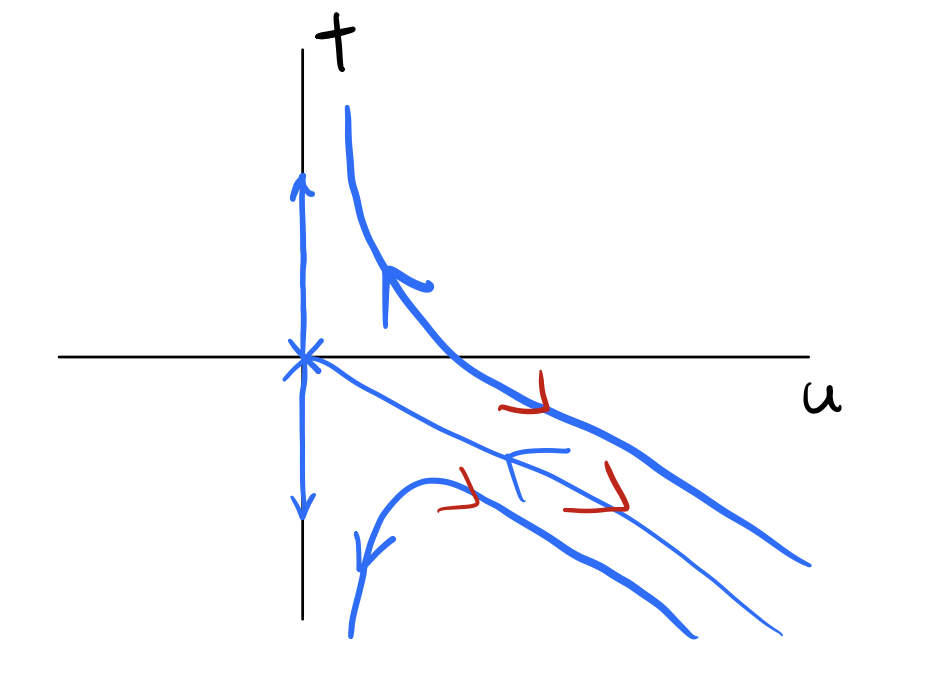
\includegraphics[scale=0.4]{Lectures/Figures/rgflow-linear.png}
    \caption{Flow for linearized RG; for $d > 4$ $u$ flows towards $0$, but for $d < 4$ $u$ diverges to infinity.}
    \label{rgflow-linear}
\end{figure}

There are also second order terms - we will not look at these as there are 36 terms and this will be painful. But we sort of know what to expect. There will be corrections of order $u^2$, so:
\begin{equation}
    \dod{t}{l} = 2 + u(\text{factor}) - Au^2
\end{equation}
\begin{equation}
    \dod{u}{l} = u(4-d) - Bu^2
\end{equation}
Now, if $u$ starts to flow away from the origin, it will get pushed back! In that case, what happens is we get a new critical point at $u^*$, which is equal to:
\begin{equation}
    u^* = \frac{4-d}{B}
\end{equation}
which is where $u$ stops flowing. There will be a corresponding critical value $t^*$:
\begin{equation}
    t^* \sim -Cu^ + \text{(corrections)}
\end{equation}

\begin{figure}[htbp]
    \centering
    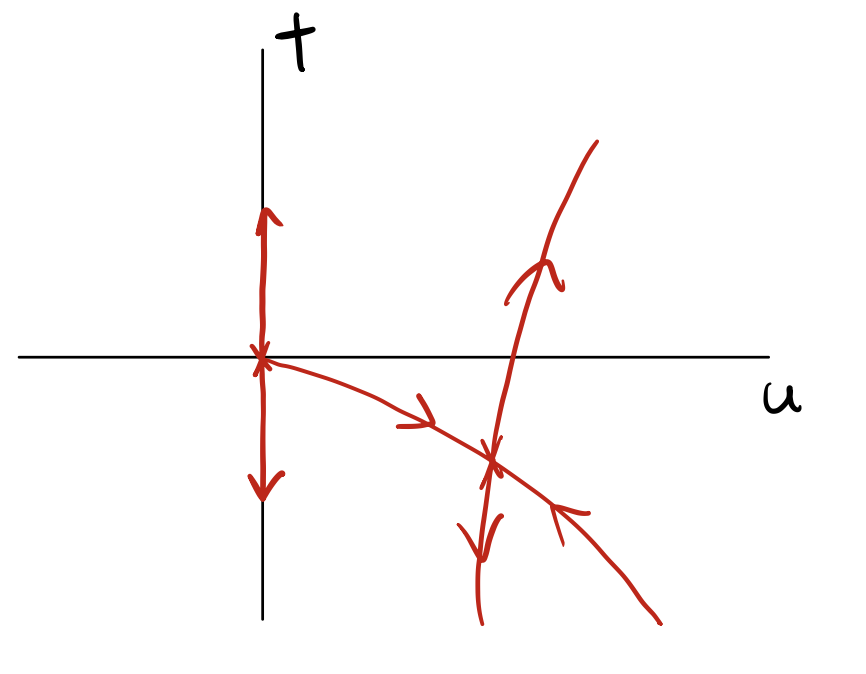
\includegraphics[scale=0.4]{Lectures/Figures/rgflow-quadratic.png}
    \caption{Flow for RG to quadratic order; a new fixed point emerges.}
    \label{rgflow-quadratic}
\end{figure}


This is a rather laborious calcualtion to show this, but it has been done. But what is important to note is that in principle the behaviour is controlled by $4-d$, and if we define $\e = 4-d$, then this is what is known as the $\e$-expansion, i.e. regularizing the problem by working close to a critical dimension:
\begin{equation}
    u^* = \frac{\e}{B}
\end{equation}
The result of which is:
\begin{equation}
    y_t = 2 - \frac{n+2}{n+8}\e + O(\e^2)
\end{equation}
\begin{equation}
    y_u = -\e
\end{equation}
This is a manifestation of universality (I missed why this was...)

One should also check what other kinds of coefficients get generated by this process. If we keep going on, there will be terms of $\e^2$, and we will generate other gradient terms we did not have before. They will always appear one order higher than the previous. At this level, the new fields are generated and are irrelevant at this order.

What happens if we try $\e = 1$ do get $d = 3$? The exponents turn out for Ising model are remarkably close to numerical estimates, even though there is no reason things should have been. We don't know what the radius of convergence of this series is; it is a bit of a punch in the dark. 

Note that the fixed point $(t^*, u^*)$ is the known as the Wilson-Fisher fixed point.

Reviewing exactly what we have done today:
\begin{itemize}
    \item We take a model that has a complicated higher order term, namely the fourth order term.
    \item What we know is that this term can be made small by going into the vicinity of a critical dimension, here $d = 4$. (The scaling dimension of the fourth order term is $4-d$). To the extent that this is a small number, the expansion can be controlled.
    \item Then, we know that the scaling law has to be augmented as we go through perturbatively through terms, with corrections $u, u^2, \ldots$. Therefore the $\dod{t}{l}$ must have the power series functional form that we found. \item The signs of the term we do not necessarily know, but we can guess that we can find solutions by postulating that there exist fixed points of the form as we found.
    \item Then we get a scaling diagram, where in addition to the Gaussian fixed point (unstable in the $u$ direction) we find the Wilson-Fisher fixed point, which $u$ flows to.
    \item Rather than the tedious algebra, the takeaway is the structure of the theory that comes out of it, and what kind of scaling theory it gives us.
\end{itemize}

Next class, we will look at continuous symmetries, which are slightly easier to deal with. We go away from spin waves, towards objects with topology. We shall begin this with the nonlinear-$\sigma$ model (spins of fixed length that can point in any direction). From there, we will go to the 2-D $XY$ model, and start to study topology in spin space.
\section{Continuous Symmetries - Beyond Spin Waves}
We return back to models with Goldstone modes and transverse fluctuations, where:
\begin{equation}
    S_t(q) \sim \frac{1}{q^2}
\end{equation}
for $T < T_c$. These are models where the order parameters have a $U(1)$ symmetry - order parameters of the form:
\begin{equation}
    \psi(r) = \abs{\psi}e^{i\theta}
\end{equation}
and correlation functions look like:
\begin{equation}
    \avg{\Theta(q)\Theta(q')} = \frac{\delta(q + q')}{q^2}
\end{equation}
Where:
\begin{equation}
    \avg{\Theta(r)\Theta(0)} \sim \begin{cases}
        r^{2-d} & d < 2
        \\ \ln r & d = 2
        \\ C & d > 2
    \end{cases}
\end{equation}
The $d = 2$ case is confusing because its not clear what the $\ln r$ means. One route into thinking about this is thinking about models where we can apply RG. 

\subsection{Non-linear $\sigma$ models}
We consider the non-linear $\sigma$ model (kind of a misnomer - Gell-Mann named it because he thought it would describe $\sigma$-mesons, even though it does not, but the name stuck). Here, we consider an $n$-component spin of length 1. We can thus write the spin degrees of freedom as:
\begin{equation}
    \v{s} = (s_1, s_2, \ldots s_n)
\end{equation}
where:
\begin{equation}
    \sum_i \abs{s_i}^2 = 1
\end{equation}
$n = 2$ would be the $XY$-model, $n = 3$ would be the Heisenberg model, and we can be in arbitrary dimension. Each one of these components should have a transverse mode.

We can write down the partition function for this as follows:
\begin{equation}
    Z = \int \mathcal{D}\left[\v{s}(x), \delta(\abs{\v{s}}^2 - 1)\right]\exp(-\frac{k}{2}\int_{\Lambda}\abs{\nabla s}^2 dx)
\end{equation}
Note that the stiffness $k$ is a function of temperature, namely $k \sim \frac{1}{T}$.

We integrate over all possible parts, maintaining the constraint that the length of the spin is unity. It is easiest to re-label spins:
\begin{equation}
    \v{s} = (\pi_1, \pi_2, \ldots, \pi_{n-1}, \sigma)
\end{equation}
i.e. pick out one component of the spins and integrate it out. The $\sigma$ component is fixed by the constraint, and so:
\begin{equation}
    \int \mathcal{D}[\v{s}(x), \delta(\abs{s}^2 - 1)] = \int \mathcal{D}\gv{\pi}\mathcal{D}\sigma \delta(\abs{\pi}^2 - \sigma^2 - 1) = \int \mathcal{D}\gv{\pi}d\sigma\left[\delta(\sigma - \sqrt{1 - \pi^2})\delta(\sigma + \sqrt{1 - \pi^2})\right] = \int \frac{1}{2}\frac{\mathcal{D}\gv{\pi}}{\sqrt{1 - \pi^2}}
\end{equation}
So then we can write $Z$ as:
\begin{equation}
    Z = \int \frac{\mathcal{D}\pi(x)}{\sqrt{1 - \pi(x)^2}}\exp(-\frac{\kappa}{2}\int d^dx \left[(\nabla \pi)^2 + (\nabla(\sqrt{1 - \pi^2}))^2\right])
\end{equation}
The last thing to do is to get rid of the pesky $\frac{1}{\sqrt{1 - \pi(x)^2}}$ term and exponentiate:
\begin{equation}
    Z = \int \mathcal{D}\pi \exp(-\frac{\kappa}{2}\int d^dx \left[(\nabla \pi)^2 + (\nabla(\sqrt{1 - \pi^2}))^2\right] + \frac{\rho}{2}\ln(1 - \pi^2))
\end{equation}
where $\rho = 1$. So far this is exact with no approximations. But of course, we will not get much further without doing an expansion. 

To leading order, we find:
\begin{equation}
    \avg{\pi^2}_0 = T
\end{equation}
as as $T \to 0$, the occupation of the Goldstone modes goes to zero. By expanding, we have:
\begin{equation}
    \beta H = \beta H_0 + u_1 + u_2 + \ldots
\end{equation}
where:
\begin{equation}
    \beta H_0 = i\int d^dx \frac{1}{2}\kappa(\nabla \pi)^2
\end{equation}
and:
\begin{equation}
    u_1 = \int d^{d}x\left[\frac{1}{2}\kappa(\pi \nabla \pi)^2 - \rho \frac{\pi^2}{2}\right]
\end{equation}
We now have an opportunity to go through RG, but in a bit of a different way; the $(\pi \nabla \pi)^2$ terms should get smaller and smaller.

Let's take this and go into Fourier space:
\begin{equation}
    \beta H_0 = \frac{\kappa}{2}\int \frac{d^dq}{(2\pi)^d}q^2\abs{\pi(q)}^2
\end{equation}
\begin{equation}
    u_1 = -\frac{\kappa}{2}\int \frac{d^dq_1 \ldots d^dq_4}{(2\pi)^{4d}} \delta(\sum_i q_i)(q_1 \cdot q_3)\pi_\alpha(q_1)\pi_\alpha(q_2)\pi_\beta(q_3)\pi_\beta(q_4) - \frac{\rho}{2}\int \frac{d^dq}{(2\pi)^d}\abs{\pi(q)}^2
\end{equation}
Now we turn the RG crank.

\subsection{RG for Non-linear $\sigma$ model}
We divide up momentum space into a shell $\sigma$ (corresponding to $\Lambda/b < q < \Lambda$) and the rest (corresponding to $\tilde{\pi}$), and integrate out that shell. Each $\pi$ term appearing above can be broken up into a $\tilde{\pi}$ part and a $\sigma$ part. The only terms which will survive will be the ones where $\sigma$ come in pairs. For example, we will have a Gaussian average of the form:
\begin{equation}
    \avg{\sigma_\alpha(q_1)\sigma_\alpha(q_2)}\pi_\beta(q_3)\pi_\beta(q_4)
\end{equation}
Actually, we will only have two surviving parts:
\begin{equation}
    \begin{split}
        (A) &= -\frac{\kappa}{2}\int d^dq_1 \ldots d^dq_4 (q_1 \cdot q_3)\avg{\sigma_\alpha(q_1)\sigma_\alpha(q_3)}\tilde{\pi}_\beta(q_2)\tilde{\pi}_\beta(q_4)
        \\ &= -\frac{\kappa}{2}\int d^dq_1 \ldots d^dq_4 (q_1 \cdot q_3)\delta(q_1 - q_3)\tilde{\pi}_\beta(q_2)\tilde{\pi}_\beta(q_4)
        \\ &= \frac{\kappa}{2}\int_{\Lambda/b}^\Lambda d^dk \frac{k^2}{\kappa k^2}\int_0^{\Lambda/b}\frac{d^dq}{(2\pi)^d}\abs{\tilde{\pi}(q)}^2
    \end{split}
\end{equation}
in the last line $k = q_1 = q_3$ and $q = q_2 = q_4$. We use the known expectation value of the $\sigma$s from our previous analysis. There is also a $(n - 1)$ factor coming from the components of the spin, which we don't write above. The other surviving part is:
\begin{equation}
    \begin{split}
        (B) &= -\frac{\kappa}{2}\int d^dq_1 \ldots d^dq_4(q_1 \cdot q_2)\tilde{\pi}_{\alpha}(q_1)\tilde{\pi}_\beta(q_3)\avg{\sigma_\alpha(q_2)\sigma_\alpha(q_4)}
        \\ &= \frac{\kappa}{2}\int \frac{d^dq}{(2\pi)^d}q^2\abs{\tilde{\pi}(q)}^2 \frac{I_d}{\kappa}
    \end{split}
\end{equation}
where:
\begin{equation}
    I_d = \int_{\Lambda/b}^\Lambda d^dk \frac{1}{k^2}
\end{equation}
We have two things that are changing here, $\kappa$ and $\rho$, which we renormalize:
\begin{equation}
    \tilde{\kappa} = \kappa\left[1 + \frac{I_d(b)}{\kappa}\right]
\end{equation}
\begin{equation}
    \tilde{\rho} = \rho[1 - b^{-d}]
\end{equation}
where:
\begin{equation}
    \rho = \frac{N}{V}\int_0^\Lambda \frac{d^dq}{(2\pi)^2}
\end{equation}
Then, the two terms we had before become:
\begin{equation}
    -\beta H' = -\tilde{\kappa}\frac{b^{d-2}}{2}z^2 \int d^d x (\nabla\pi)^2
\end{equation}
\begin{equation}
    u_1' = -\kappa\frac{b^{d-2}z^4}{2}\int d^dx (\pi \nabla \pi)^2 + \frac{\rho z^2}{2}\int d^dx \abs{\pi(x)}^2
\end{equation}
Looking at the average:
\begin{equation}
    \avg{\tilde{s}}_0 = \avg{(\pi_1 + \sigma_1)(\pi_2 + \sigma_2)\ldots \sqrt{1 - (\tilde{\pi} + \sigma)^2}} = 1 - \frac{1}{2}\avg{\sigma}^2 + O(T)^2 = 1 - \frac{n-1}{2}\frac{I_d(b)}{\kappa} = z
\end{equation}
This tells us that we have to choose the scaling exponent (that sets the size of the spin, which is fixed!) such that the above is preserved, hence we set the above to $z$. Then:
\begin{equation}
    \kappa = b^{d-2}z^2\tilde{\kappa} = b^{d-2}\left[1 - \frac{n-1}{\kappa}I_d\right]^2\kappa\left[1 + \frac{I_d}{\kappa}\right] = b^{d-2}\kappa\left[1 - \frac{n-2}{\kappa}I_d + O(\frac{1}{\kappa^2})\right] + \ldots
\end{equation}
So then $b \sim e^{l}$, and:
\begin{equation}
    \dpd{\kappa}{l} = (d-2)\kappa - (n - 2)\kappa \Lambda^{d-2}
\end{equation}
so temperature scales to zero or infinity here depending on dimension and the number of components.

Say, take $d < 2$. Then $\kappa \to 0$ so $T \to \infty$ and no order. But, for $d > 2$, we have $\kappa \to \infty$ so $T \to 0$ and we are ordered. The critical temperature is then:
\begin{equation}
    T^* = \frac{d-2}{n-2}\frac{1}{\kappa_0\Lambda^{d-2}}
\end{equation}
At $n = d = 2$ we have the XY-model which is not resolved. 
% $n = 1$ the order depends on the dimension, for $d = 1$ no order but for larger dimensions we do get order.

\subsection{Vortices}
What have we missed in the spin wave theory? Consider $d = 2, n = 2$. There are objects in the lattice where there are vortices; faraway it looks like the spin just slowly varies, but close to it there is an observable ``vortex charge'' measurable by going around it in a loop. There are charges and anti-charges, and we measure these via:
\begin{equation}
    \oint_S \nabla \theta \cdot d\v{s} = (2\pi)m
\end{equation}
for $m \in \ZZ$. Labelling these as charges is well-motivated; they behave like charges. In fact it will look exactly like EM. Indeed they actually form in pairs.

\begin{figure}[htbp]
    \centering
    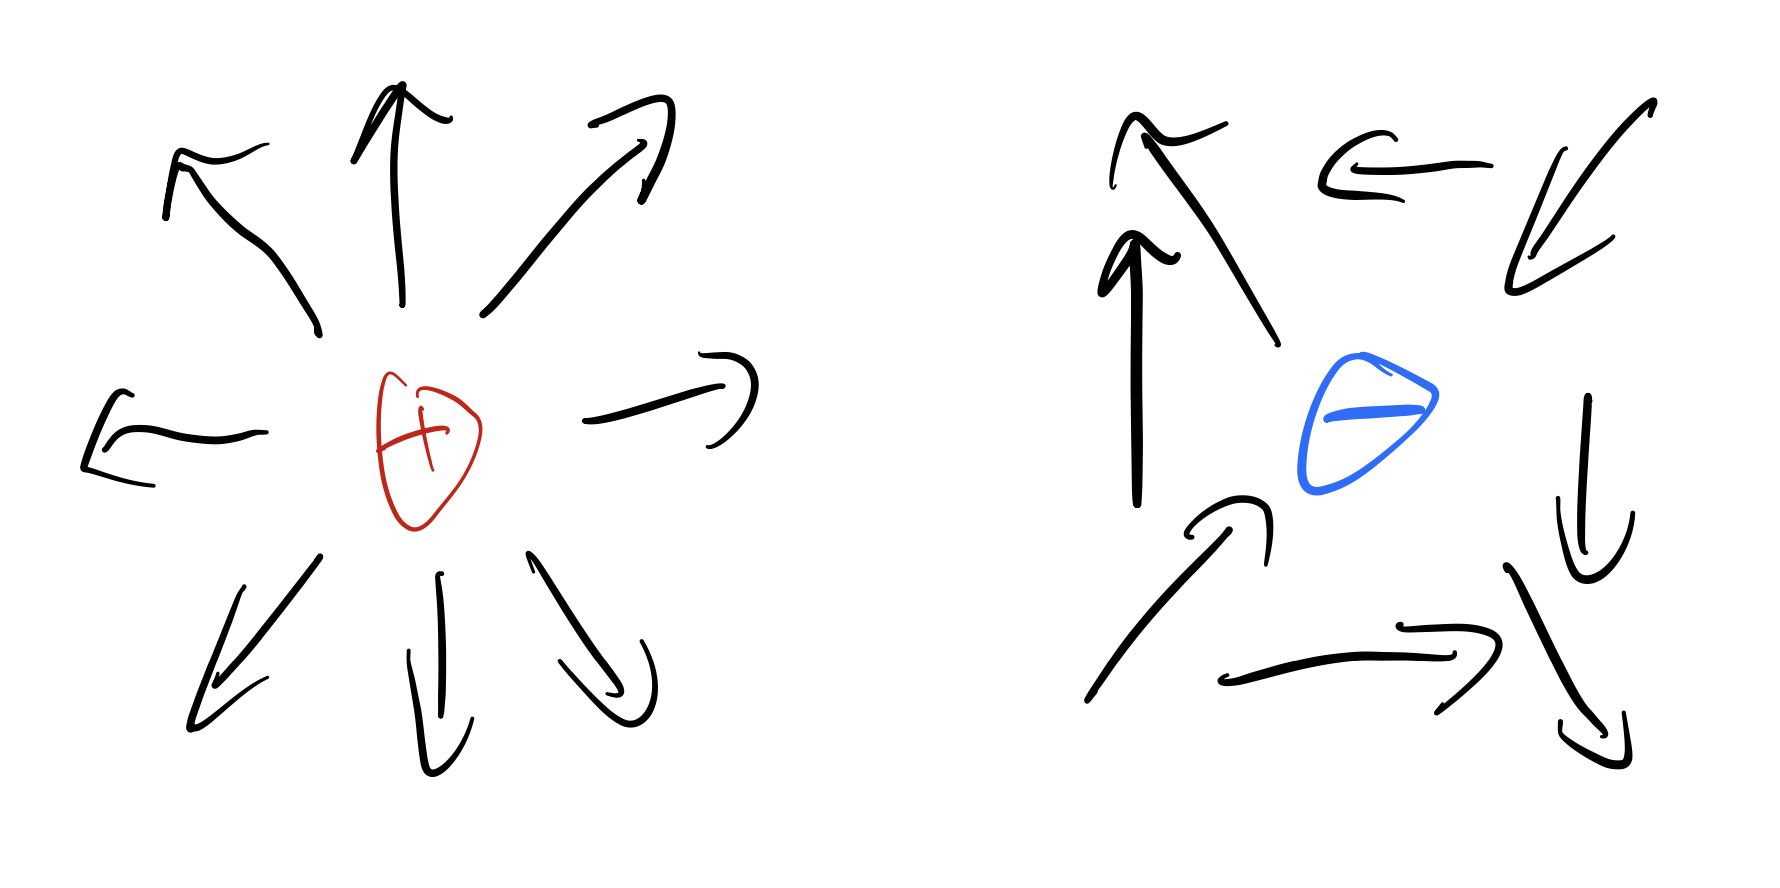
\includegraphics[scale=0.3]{Lectures/Figures/vortexcharges.png}
    \caption{Cartoon picture of spin vortex charges}
    \label{fig:vortexcharges}
\end{figure}

We can ask; does it make sense that as we go down to low $T$ we have the spontaneous formation of these vortices? Normally, one would think that it takes finite energy to place them in the lattice (so they should go away at low $T$) but there are so many places to put them and as such there is an entropic gain as well... What happens is (even at low $T$) fluctuations create charges out of a vacuum, but they will be close together and be bound. This is one phase. There is also a second possible phase where the charges unbind; we go from vortex charge molecules to a plasma; they begin to overlap, and they start screening, and the system breaks itself up. We can describe this with classical EM. This transition/plasma phase has no long range order, but the confined phase has a quasi-long range order, where the effective stiffness stays finite. The transition between these two is the Berezinskii-Kosterlitz-Thouless transition.
\section{2-D XY model}
\subsection{Single Vortices}
Let us recap where we ended up last class. What has been missing thus far from our discussion of continuous systems is the presence of vortices. We were assuming that we could capture everything with slow variations of spins, but this leaves out configurations like those that appear in Fig. \ref{fig:vortexcharges}. We can define such vortices by looking at:
\begin{equation}
    \oint (\nabla \theta) \cdot d\v{S} = 2\pi n
\end{equation}

We can make vortices that wind more than once, or those that have negative $m$ (antivortices). Since:
\begin{equation}
    \nabla \theta  = -n\nabla \times (\zhat \ln r) \sim \frac{1}{r}
\end{equation}

Let's compute the energy of a vortex.

\begin{equation}
    \beta \mathcal{E}_m = \beta \mathcal{E}_0(a) + \frac{1}{2}\kappa\int_a^L d^2x (\nabla \theta)^2 = \beta \mathcal{E}_0(a) + \pi \kappa n^2 \ln(L/a)
\end{equation}
which diverges in the system size. This may suggest that we might not have any vortices - but this is not the case. Let's look at the partition function:
\begin{equation}
    Z(n) \approx \left(\frac{L}{a}\right)^2 e^{-\beta \mathcal{E}_0(a)} e^{-\pi \kappa n^2 \ln(L/a)}
\end{equation}
The $\mathcal{E}_0(a)$ is like the chemical potential, and we can call its exponential the fugacity. We have:
\begin{equation}
    Z(n) \approx y_0(a) \left(\frac{L}{a}\right)^{2 - \pi\kappa n^2}
\end{equation}
Let us also remember that $\kappa \propto \frac{1}{T}$. So, above $T_c \sim \frac{\pi}{2}n^2$ is where the vortices proliferate (look at the term in the partition function). Although the energy contribution is infinite, the entropic gain wins out at this temperature.

\subsection{Pairs of Vortices}
This was a single vortex; there are also pairs of vortices, which is what we will have to pay attention to. Consider a vortex anti-vortex pair at distance $d$. We then find:
\begin{equation}
    (\nabla \theta) \sim d \nabla\left(\frac{\v{r} \times \v{z}}{r}\right) \sim \frac{1}{r^2}
\end{equation}
These have finite energy, and act like a Coloumb gas.

Consider a flow, which we treat by looking at a sum of a rotational and irrotational part.
\begin{equation}
    \v{u}(\v{r}) = \nabla \theta 
\end{equation}
One part is curl free (this is the piece without vortices):
\begin{equation}
    (\nabla \times u_0) = 0 \implies u_0 = \nabla \phi
\end{equation}
Then:
\begin{equation}
    u = u_0 - \nabla \times (\v{z} \psi)
\end{equation}
where if we consider the contribution from vortices:
\begin{equation}
    \oint \v{u} \cdot d\v{S} = 2\pi \zhat \sum_i n_i \delta(r - r_i)
\end{equation}
Then:
\begin{equation}
    \nabla \times \v{u} = \zhat \nabla^2 \psi
\end{equation}
We can then see:
\begin{equation}
    \nabla^2 \psi = 2\pi \sum_i n_i \delta(r - r_i)
\end{equation}
So then:
\begin{equation}
    \psi(r) = \sum_i n_i \ln(\abs{r - r_i})
\end{equation}
Having written the field as this, let us compute the energy:
\begin{equation}
    \beta H = \frac{1}{2}\kappa \int d^2r \left[(\nabla \phi)^2 - 2(\nabla \phi) \cdot \nabla(\zhat \psi) + (\nabla \times \zhat\psi)^2\right]
\end{equation}
The middle term vanishes via integrating by parts. The first term is familiar. The third term looks like:
\begin{equation}
    (\nabla \times \zhat\psi)^2 = \left(-\dpd{\psi}{x}, \dpd{\psi}{y}, 0\right)^2 = (\nabla \psi)^2
\end{equation}
We then have (through an integration by parts):
\begin{equation}
    \beta H_1 = \kappa \int d^2r (\nabla \psi)^2 = -\frac{\kappa}{2}\int d^2 r \psi \nabla^2 \psi = -\frac{\kappa}{2}\int d^2r (\sum_i n_i \ln(\abs{r - r_i}))(\sum_j 2\pi n_j \delta(r - r_j))
\end{equation}
which we can now use to define the correlation function:
\begin{equation}
    \beta H_1 = -\frac{\kappa}{2}\int d^2r \sum_{i\neq j} n_i n_j C(r_i - r_j)
\end{equation}
where:
\begin{equation}
    C(r_i - r_j) = \frac{\ln(\abs{r_i - r_j})}{2\pi}
\end{equation}
and we exclude a vortex interacting with itself.

\subsection{Transitions}
Now, we may go back and write down the full partition function:
\begin{equation}
    Z = \int \mathcal{D}\phi e^{-\frac{\kappa}{2}\int (\nabla \phi)^2}\sum_{r_k}\int d^2r_k e^{-\sum_i \beta\mathcal{E}_0(r_i) + 4\pi^2\kappa \sum_{ij} n_i n_j C(r_i - r_j)}
\end{equation}
The first term corresponds to spin waves, and the second corresponds to vortices, so we can write:
\begin{equation}
    Z = Z_{SW}Z_{\text{vort}}
\end{equation}
We also constrain the configuration to that which where $\sum_i n_i = 0$, and restrict to $n_i = \pm 1$. To make the connection with charges more clear, we replace $n_i$ with $q_i$. We then study:
\begin{equation}
    Z_v = \sum_{N=0}^\infty (y_0)^N \int \prod_{k=1}^N d^2r_k \exp(4\pi^2\kappa\sum_{ij}q_iq_jC(r_i - r_j))
\end{equation}

Suppose the fugacity is small, such as in a metal-insulator. Then, $y_0$/the fugacity is small ($y_0$ can be thought to be controlling the density), and we should see that the vortices bind in pairs. Here, $C(x) \to C(x)/\mathcal{E}$. There is another limit where $y_0$ is large, and then the bound pairs of charges start to overlap highly, so much so that the charges become unbound. This is the plasma phase. and we see $C(x) \sim e^{-x/\xi}$. 

We have:
\begin{equation}
    Z \sim y_0(a) \left(\frac{L}{a}\right)^{2-\pi\kappa} \to y_0(ba)\left(\frac{L}{ba}\right)^{2 - \pi \kappa}
\end{equation}
where we rescale such that the partition function remains invariant. Then if we make $b \sim e^{-\delta l}$:
\begin{equation}
    \dod{y_0}{l} = (2 - \pi \kappa)y_0
\end{equation}
The $x = 2 - \pi \kappa$ parameter tells us whether vortices are relevant or not.

We then assert:
\begin{equation}
    \dod{x}{l} = Ay_0^2
\end{equation}

Which gives rise to the flow diagram:

\begin{figure}[htbp]
    \centering
    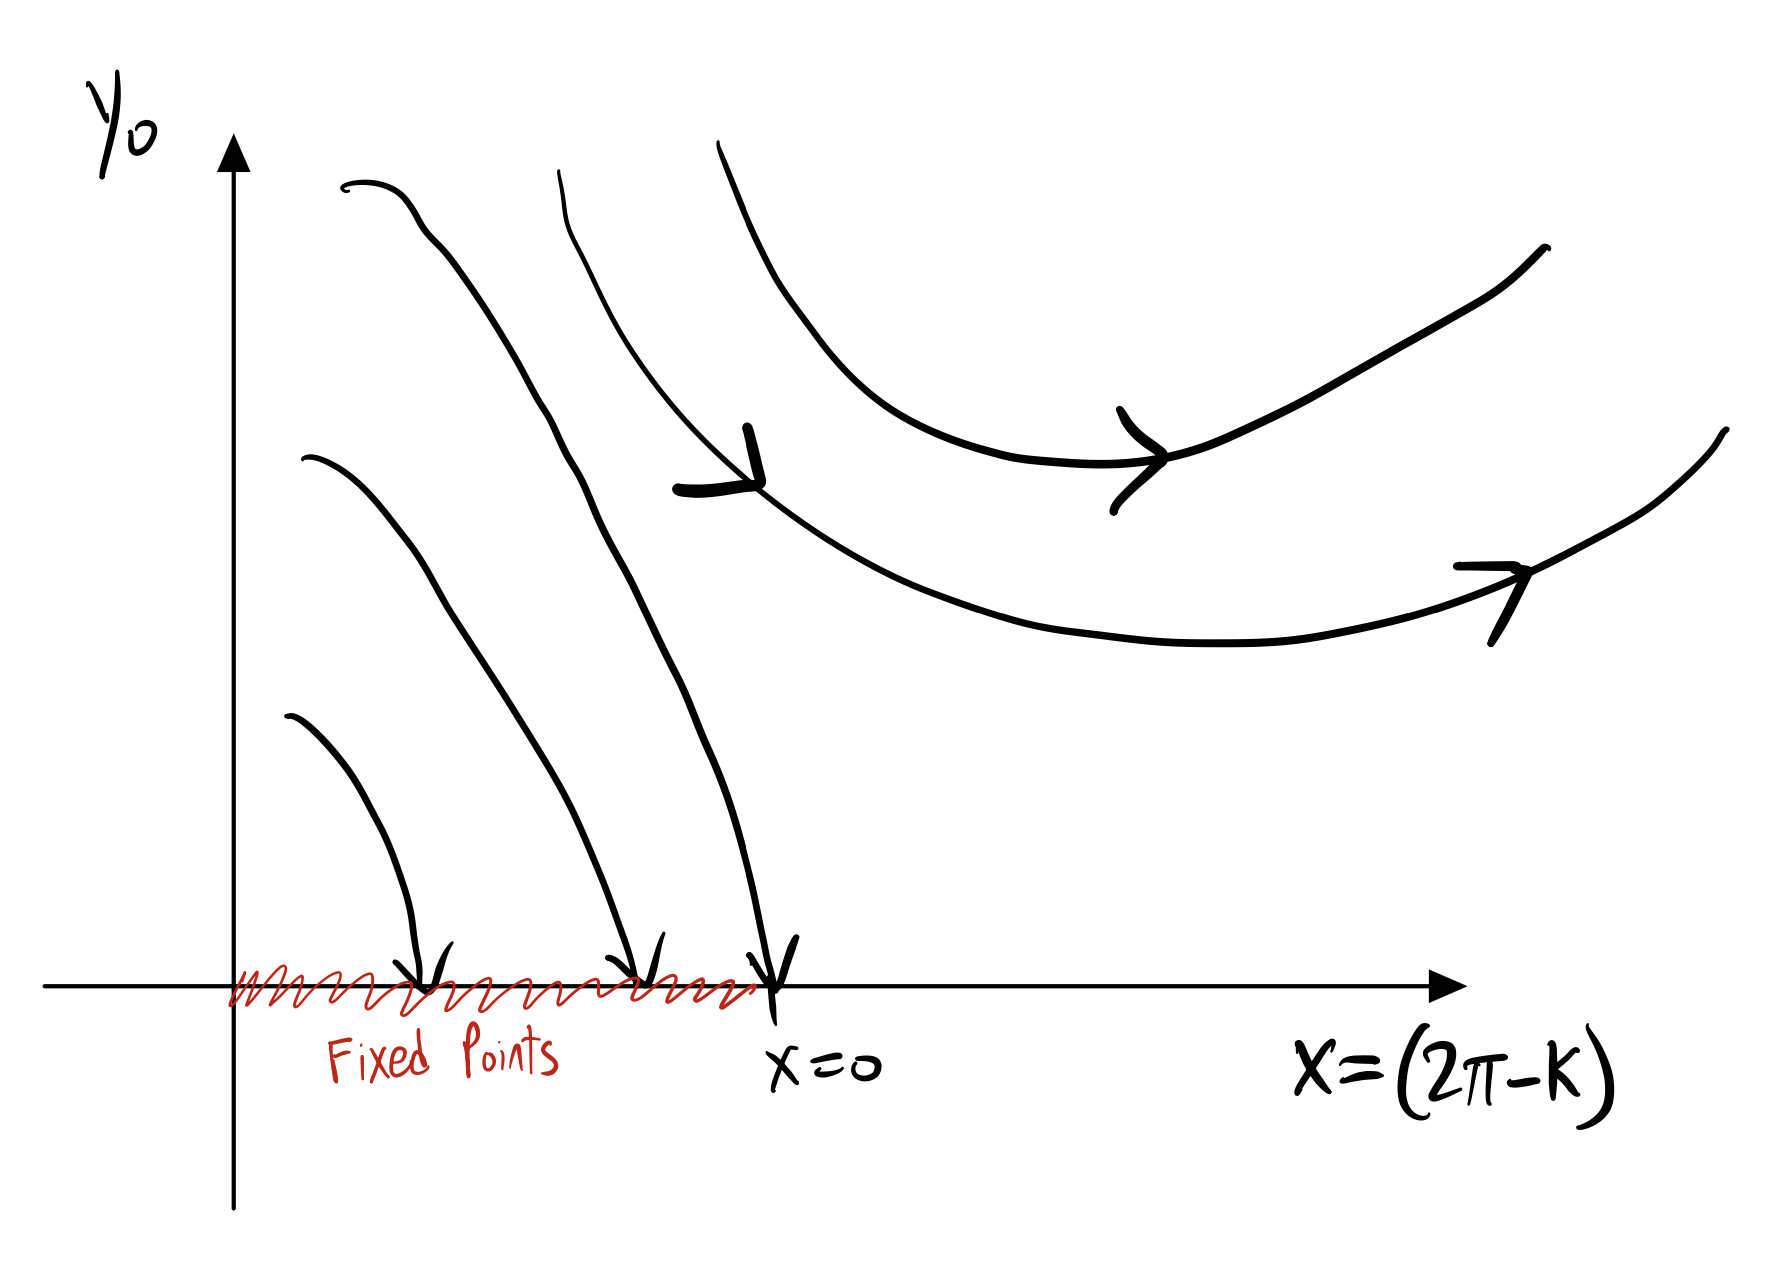
\includegraphics[scale=0.3]{Lectures/Figures/xymodelflow.png}
    \caption{Flows of fugacity and stiffness in the 2-D XY model, corresponding to 2 different phases with differing behaviour of vortices.}
    \label{fig:xymodelflow}
\end{figure}

So we have two regimes, one where vortices are irrelevant and another where they proliferate. There is a separatrix line which is the dividor between whether we flow to no vortices or proliferation. We can say this defines a physical transition temperature, known as the Berezinskii-Kosterlitz-Thouless temperature.

Lastly, let us think about what the correlation functions look like:
\begin{equation}
    \avg{\psi(r)\psi(0)} = \frac{1}{r^{1/2\pi\kappa}}
\end{equation}
Notice that this power law varies. When we get to $k = 2/\pi$, at that point the correlator goes as $\sim \frac{1}{r^{1/4}}$. But, everywhere along the line of $x = 0$ fixed points there is a (continously varying) power law (i.e. each point along the line has a different critical exponent), up until $r^{-1/4}$, at which afterwards it becomes a short-range correlator $e^{-r/\xi}$ which exponential decay. This means, at the transition temperature, there is a jump in physical properties.

\subsection{Polarizability + Looking ahead}

Suppose we add an external field:
\begin{equation}
    H = H_0 + \v{E} \cdot \sum_{\v{R}} \v{R} \cdot n(R)
\end{equation}
Suppose now we want to compute the dielectric function:
\begin{equation}
    \chi_{ij} = \frac{\partial f}{\partial E_i \partial E_j} \sim \sum \sum_{\v{R}}R^2\avg{n(R)n(0)} = \int dR R^3 e^{-2\pi\kappa \ln(R)} = \int_a^L dR R^{3-2\pi\kappa} L^{4-2\pi\kappa}
\end{equation}
which depending on $\kappa$ either diverges or vanishes. It diverges when $\kappa = 2/\pi$. This connects back up to the correlation function above.

Next day, we move to disorder and randomness. Everything we have talked about thus far assumes a perfect medium and translational invariance. We will now break this. This is both relevant in a practical sense (every physical system has disorder of some form), and also inherently interesting problems with disorder, e.g. frustration. We could consider models with sufficient randomness such that the spins have confusion about their orientation, then we can get systems that act glassy - they freeze into a disorder state. There is a sharp transition from a slowly-flowing material to something that freezes; this is called a spin glass, and we will talk about the infinite-range spin-glass, which we will be able to solve exactly (the Parisi solution - he won a Nobel prize for this)! Interestingly, these kinds of models allow you to store information/use them as a physical memory, which was John's Hopfield's idea. Rapidly coming out of this was how one ``learns'' via tuning parameters, the simplest of which is the Boltzmann machine. Of course, this was the Nobel prize in physics this year.
\section{Disorder and Random Systems}

\subsection{Introduction and Motivation}
Disorders and imperfections are unavoidable in real systems; do phase transitions still exist in this setting? This will be the first point which we will address, and we will be able to answer it quite sharply.

The answer will turn out to be yes, but we then have the follow-up question; how are the transitions modified? We will find that the (upper and lower) critical dimensions become modified.

Finally, we may ask if there will be new phenomena emerging from disorder; indeed there can be, and we will look at the example of a glass, where there is an abrupt transition to being frozen/carrying information.


\subsection{Disorder Type I - Impurities/Vacancies}
E.g. we have a ferromagnet, and randomly start removing spins. We could for example write down the Hamiltonian:
\begin{equation}
    H(\set{s},\set{m}) = -\frac{1}{2}\sum_{ij}J_{ij}s_is_jm_im_j
\end{equation}
where randomly, we pick sites $m_i$ and set them to zero such that those terms become absent from the sum. We will need to make a careful distinction about whether the system is quenched or annealed. Suppose we ``freeze in'' the spin configuration. Then the partition function looks like:
\begin{equation}
    Z(\set{m}) = \Tr_S e^{-\beta H(s, m)}
\end{equation}
which is called ``quenched''. This has the odd feature that the answer depends explicitly on the $\set{m}$. If we do the experiment again and put the impurities in different places, we get a different partition function. We could instead construct the ``annealed'' partition function, which is:
\begin{equation}
    Z = \Tr_m Z(\set{m})
\end{equation}
where we average over all configurations $\set{m}$ of empty sites. The annealed problem is a tough one and we won't address it in this lecture, but we will attack the quenched partition function.

A comment - we lose translational invariance when we do this.

Let us block our system. We can consider an averaged free energy:
\begin{equation}
    \bar{F} = \Tr_m Z[\set{m}]F[\set{m}]
\end{equation}
where we assume that we can compute (over a given block) $F[\set{m}]$ governed by $P[\set{m}]$ (each block will have a different value, but obeys the same distribution). The $\bar{F}$ above represents a quenched average. Looking at the probability distribution, we have:
\begin{equation}
    P[\set{m}] = \prod_i \left[(1 - x)\delta_{m_i 1} + x \delta_{m_i0}\right]
\end{equation}
where $x$ is is the concentration of vacancies. The important thing to think about; when we do the trace over $S$, we average over spin configurations, but do not minimize over the free energy. It is instead, fixed here.

We distinguish the thermal average with the spatial average:
\begin{equation}
    \avg{s_is_j} \neq \overline{\avg{s_is_j}}
\end{equation}
where the lhs represents the thermal average, the rhs the spatial. The thermal average is dependent on the spin configuration, but the spatial average only depends on the distance between $i, j$ i.e. $\abs{i - j}$. Formally, we can write:
\begin{equation}
    \overline{\avg{s_is_j}} = \frac{1}{N}\sum_k \avg{s_{k+i}, s_{k+j}} = M(\abs{i-j})
\end{equation}
why might we want to do this? It is relevant for determining magnetic fluctuations in the system.

We can consider some types of impurities/vacancies:
\begin{enumerate}[(i)]
    \item Bond dilution, e.g. $J_{ij} = J + \text{small fluctuations}$.
    \item Random field; $H = \sum_{ij}J_{ij}s_is_j + \sum_i h_i s_i$ where we make the $h_i$ random. Where $\bar{h} = 0$ and $\overline{hh} = \Delta$.
    \item Spin glass, where we take $J_{ij}$ random with mean zero. In this case, since we pick couplings randomly, we can have frustrated systems. Note that is similar to bond dilution with $J = 0$, but allowing the fluctuations to be not necessarily small. We could call a system with $s_i(0)s_i(t) \neq 0$ a glass (correlations get ``baked in'').
\end{enumerate}

\subsection{Computing quenched averages - Replica Trick}
We want to compute:
\begin{equation}
    \bar{F} = \Tr_m P[\set{m}]\ln Z[\set{m}]
\end{equation}
averaging logarithms is hard, but we can expand $\ln Z$ in a power series:
\begin{equation}
    \ln Z = \lim_{n \to 0}\frac{Z^n - 1}{n}
\end{equation}
Taking quenched averages of power series of $Z$ are much easier. We interpret this as taking our Hamitonian and \emph{replicating}it:
\begin{equation}
    \overline{Z^n} = \Tr_m \Tr_{s^a} P[\set{m}] e^{-\sum_{a=1}^n H[\set{s^a}, \set{m}]}
\end{equation}
Because $P[\set{m}]$ is random, this will correspond to some SM model with randomness. But the trick is that we can now do the average over $m$ first, so we end up with:
\begin{equation}
    \overline{Z^n} = \Tr_{s^a}e^{-\sum_{ab}H_{\text{eff}(s^a, s^b)}}
\end{equation}
where by doing the average over $m$ we get correlations between the different replicas. (Note that in principle we could have couplings between higher numbers of replicas, but since we started with two-body couplings, we have at most couplings between pairs of replicas).

\subsection{Transition Temperatures and Concentration}
Suppose I have some concentration of impurities $x \ll 1$, and the transition temperature $T_c$ depends on $x$. Therefore, we have:
\begin{equation}
    T_c(x) \implies \xi \sim \abs{T - T_c(x)}^{-\nu(x)}
\end{equation}
Because the system varies spatially, the concentration may be different at different locations. We thus may consider the deviation:
\begin{equation}
    \delta T_c(\v{r}) = T_c(\v{r}) - T_c
\end{equation}
Let us define a correlation function:
\begin{equation}
    W(\v{r} - \v{r}') = \overline{T_c(\v{r})T_c(\v{r}')}
\end{equation}
We now ask; as we open up the block size of the system, what happens to the correlation function?

We consider an aperture/block size $L$ such that $a \ll L \ll \text{system size}$. Then:
\begin{equation}
    (\Delta T_c)^2 = \int_a^L \frac{d^dr}{L^d}\int_a^{r_0}\frac{d^dr'}{L^d}W(\v{r} - \v{r}')
\end{equation}
where we integrate up to a characteristic length scale of the correlation $r_0$:

\begin{center}
    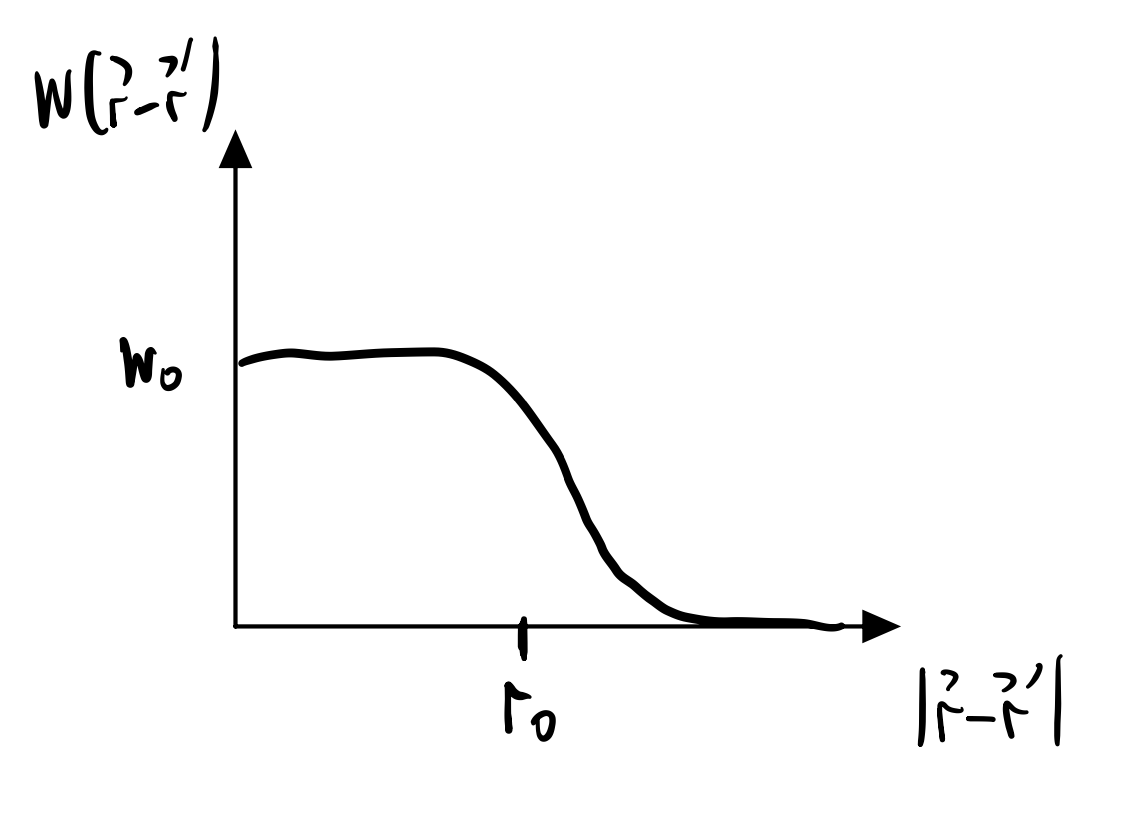
\includegraphics[scale=0.4]{Lectures/Figures/lec12-corr.png}
\end{center}

We then find;
\begin{equation}
    \Delta T_c \sim W_0^{1/2}\left(\frac{r_0}{L}\right)^{d/2} \sim \xi^{-d/2}
\end{equation}
which has the interpretation; if we average over a large volume, we have the square root number of microscopic domains in the sample. The sensible $L$ to choose here is the correlation length, because if the correlation length diverges (uniformly) this average makes sense. Thus, we should have:
\begin{equation}
    \Delta T_c \ll \abs{T - T_c(x)} \sim \xi^{-\frac{1}{\nu}}
\end{equation}
phrased another way, we want to get a convergent average when we average over the scale of the correlation length.

We thus obtain the criterion:
\begin{equation}
    \boxed{\frac{d\nu}{2} > 1}
\end{equation}
because only then will $\xi^{-d/2} \ll \xi^{-\frac{1}{\nu}}$. This is the criterion for transitions to exist, and is known as the \emph{Harris criterion}. Note that this requires $\alpha < 0$. If this is not obeyed, the phase transition is destroyed by randomness.

\subsection{Computing with Replicas}
Consider:
\begin{equation}
    H = H^* + \sum_i m_i E_i
\end{equation}
where $E_i$ is the local energy density and $m_i \in \set{0, 1}$ is the vacancy. We then have:
\begin{equation}
    \begin{split}
        \bar{Z^n} &= \Tr_m \Tr_{s^a}P(\set{m}) e^{-\sum_a H^*_a - \sum_{ia}m_i E_i^a}
        \\ &= \exp(-\sum_a H^* a -\bar{m}\sum_{ai}E_i^a + \frac{1}{2}\sum+{ab}\sum_{ij}(\overline{m_im_j} - \bar{m}^2)E_i^aE_J^b)
    \end{split}
\end{equation}
where we have used a Gaussian distribution $P(m) \sim e^{-m^2/\Delta}$ to perform the average (if not Gaussian, there are higher order terms/cumulants).

Looking at the leading off-diagonal term, we study $\sum_{a \neq b}E_i^aE_i^b$. Look at the two point function:
\begin{equation}
    \avg{\sum_{a\neq b}E_i^a E_i^b \sum_{a'\neq b'}E_j^{a'}E_j^{b'}} = 2n(n-1)\avg{E^a_iE^a_j}^2 = 2n(n-1)\frac{1}{\abs{i-j}^{4x_E}}
\end{equation}
Where $x_E$ is the critical exponent from some general operator. AS a reminder:
\begin{equation}
    \avg{\phi_\alpha(0)\phi_\alpha(r)} = \frac{1}{\abs{r}^{2x_\alpha}}
\end{equation}
with $x_\alpha = d - y_\alpha$ with $y_\alpha$ the RG eigenvalues. These come from scaling/homogeneity. This is obtained from the integral $\int d^dr'\phi(r)\phi(r+r')$. If this is associated with the energy density, then:
\begin{equation}
    x_E = d - \frac{1}{\nu}
\end{equation}
and:
\begin{equation}
    y_E = d - 2x_E = \frac{2}{\nu} - d
\end{equation}
This is the answer we get from averaging at the critical point. $y_E$ is irrelevant if $d\nu > 2$, the same answer as we got from the Harris criterion. Of course there is the pesky $n$ which if we take $n = 1$ (the limit of a simple replica) then everything goes away.

So, the story was; does the phase transition still exist? There was a heuristic argument based on averaging over a sufficiently large region that gave the Harris criterion. We could also answer this via the laborious RG procedure, which ended up giving the same answer.

If the variables are relevant the replicas get coupled, if the variables are irrelevant then the replicas remain uncoupled, and we get a trivial answer.
\section{Random Fields and Spin Glasses}
\subsection{Setting up the Random Field Problem}
We consider the Hamiltonian:
\begin{equation}
    H = \int d^dx \left(\frac{1}{2}\kappa (\nabla s)^2 + \frac{1}{2}ts^2 + \frac{1}{4}us^4 - \v{h}(x)\cdot \v{s}\right)
\end{equation}
where:
\begin{equation}
    \overline{h_i(\v{x})h_j(\v{x}')} = \delta_{ij}\Delta \delta (\v{x} - \v{x}')
\end{equation}
i.e. we have a random uncorrelated field. Although it is written down as a magnet, it is a kind of model that emerges very frequently in random media. For example, an elastic medium sitting on a surface which is random, causing the elastic to stretch in some ways.

\begin{center}
    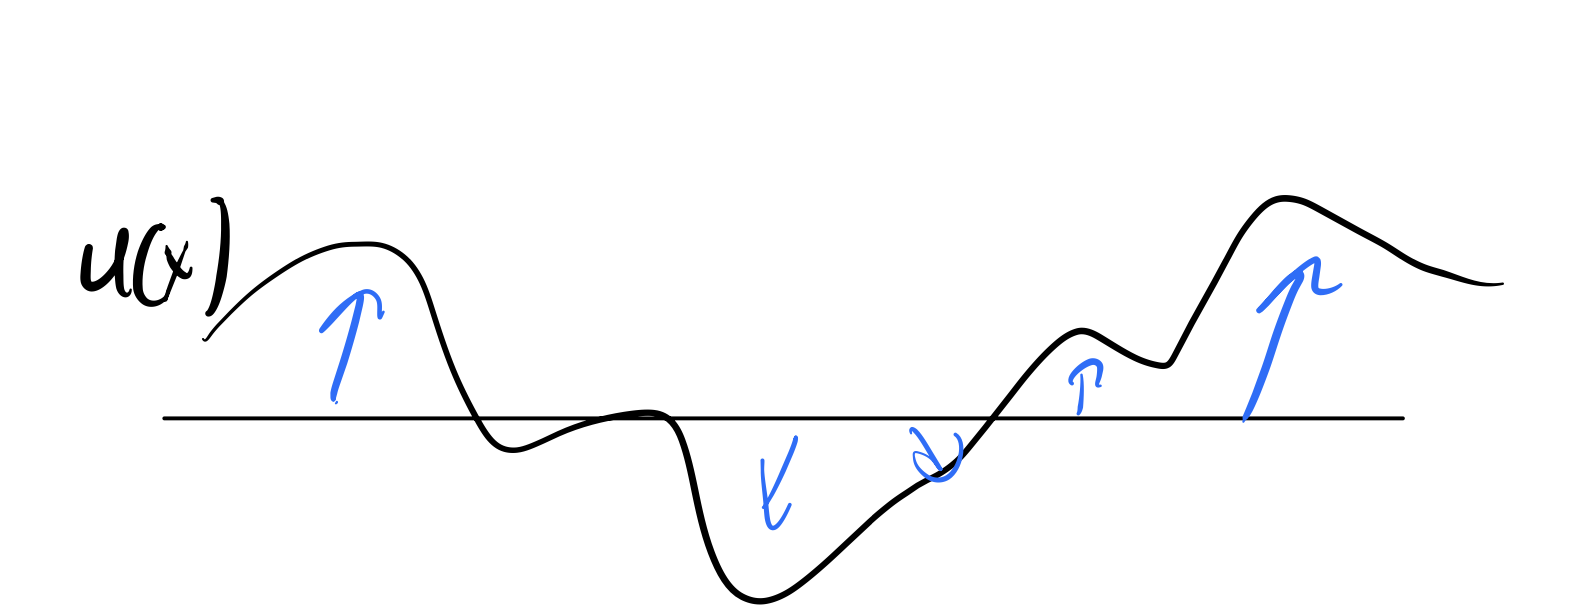
\includegraphics[scale=0.35]{Lectures/Figures/lec13-randomelastic.png}
\end{center}

Consider random fields $h_i$. If we RMS average over a length scale $L$:
\begin{equation}
    \sqrt{\sum_{i=1}^L h_i^2} = h_0\sqrt{cL^d}
\end{equation}
where $h_0$ is a strength and $c$ a concentration. This $\sim \sqrt{N}$ comes from a random walk.

If we average and get some nonzero up spin, and average in a neighbouring region and get a nonzero down spin, then we get an energy penalty. We have a gain of the form $h_0 L^{d/2}$ (from the spins within a domain aligning with the local field, from the $\v{h}_i \cdot \v{S}_i$ term) and a loss of the form $JL^{d-1}$ (coming from the penalty of interacting neighbouring domains, the $\v{S}_i \cdot \v{S}_{i+1}$ term). When do each of the terms win out? When $\frac{d}{2} > d-1$, i.e. when $d < 2$, the energy gain wins.

\subsection{Solving the model}
To attack this model, we consider the replica trick:
\begin{equation}
    \overline{Z^n} = \int \mathcal{D}h(x) P(h(x)) \prod_{a=1}^n \int dS_a e^{-\beta H[S_a, h]}
\end{equation}
We take the distribution of the fields to be Gaussian:
\begin{equation}
    P(h) \sim e^{-\frac{h^2}{\Delta}}
\end{equation}
This allows us to write:
\begin{equation}
    \overline{Z^n} = \prod_a \int dS_a e^{-\beta H_{\text{eff}}[S_a, S_b]}
\end{equation}
with:
\begin{equation}
    H_{\text{eff}} = \int d^dx\left[\sum_{a=1}^n \frac{1}{2}\kappa (\nabla s_a)^2 + \frac{1}{2}ts_a^2 + + \frac{1}{4}us_a^4\right] - \frac{1}{2}\beta \sum_{a, b}\Delta \v{s}_a \cdot \v{s}_b
\end{equation}
(Rio note: This expression doesn't looks like it makes sense with the sum over $a, b$s, but so be it.) Going to momentum space:
\begin{equation}
    H_{\text{eff}} = \frac{1}{2}\int \frac{d^dk}{(2\pi)^d}\left(\sum_{a, b}(\kappa k^2 +t)\delta_{ab}  - \beta \Delta J_{ab}\right)s_a(k)s_b(-k) + \frac{u}{4}s^4
\end{equation}
with $J_{ab}$ just a matrix of 1s everywhere. If we had no fourth order term, we can view this as a Green's function:
\begin{equation}
    \avg{s^i_a(k)s^j_b(k')} = G^0_{ab}\delta(k + k')
\end{equation}
with:
\begin{equation}
    G^0_{ab}(k) = \delta_{ij}\left[\frac{T}{\kappa k^2 + t}\delta_{ab} + \frac{\Delta}{(\kappa k^2 + t)^2}J_{ab}\right]
\end{equation}

If we study the scaling:
\begin{equation}
    \kappa \to \kappa b^{d-2+2\zeta}
\end{equation}
\begin{equation}
    t \to tb^{d+2\zeta}
\end{equation}
\begin{equation}
    u \to ub^{d+4\zeta}
\end{equation}
\begin{equation}
    \frac{\Delta}{T} \to b^{d+2\zeta}\frac{\Delta}{T} = b^2\Delta
\end{equation}
with $\zeta = \frac{2-d}{2}$ where we recall that we have the RG scaling parameters from $s \to b^\zeta s$. We see that $\Delta$ has a positive eigenvalue and is therefore a relevant exponent. There is a new relevant field in the vicinity of the fixed point, and we flow away.

\begin{center}
    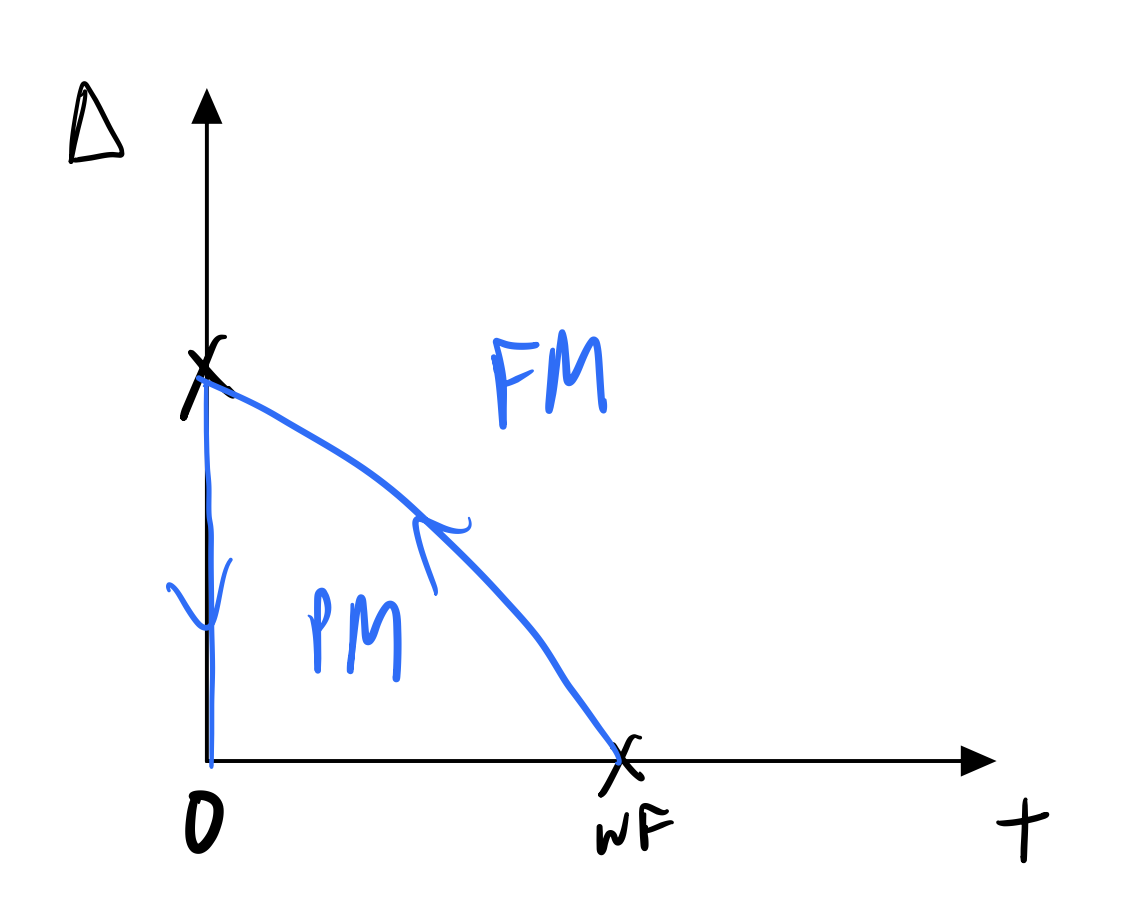
\includegraphics[scale=0.35]{Lectures/Figures/lec13-randomrgflow.png}
\end{center}

The fixed point Hamiltonian is:
\begin{equation}
    H^* = \int d^dx \left[\frac{1}{2}\kappa(\nabla s)^2\right]
\end{equation}
If we ask what is $\avg{\delta s^2}_{\text{thermal}}$, this is something we've seen before:
\begin{equation}
    \avg{\delta s^2}_{\text{thermal}} = \int_{1/L}^\infty \frac{d^dk}{(2\pi)^d}\frac{T}{\kappa k^2}
\end{equation}
Now we want to ask how this scales depending on the lower momentum cutoff $L$. By a scaling argument, we see:
\begin{equation}
    \avg{\delta s^2}_{\text{thermal}} \sim \frac{T}{\kappa}L^{2-d}
\end{equation}
If I look at the random field Hamiltonian we have the $\frac{\Delta}{(\kappa k^2 + t)^2}$ term. Then we have:
\begin{equation}
    \avg{\delta s^2}_{RF} \sim \int_{1/L}^\infty \frac{d^dk}{(2\pi)^d}\frac{\Delta}{\kappa^2k^4} = \frac{\Delta}{\kappa^2}L^{4-d}
\end{equation}
We then get the length scale over which one term wins:
\begin{equation}
    \xi = \left(\frac{\kappa}{\Delta}\right)^{\frac{1}{4-d}}
\end{equation}
In $D > 4$, this is minimized as $L \to \infty$, as $D < 4$ the length scale is finite.

Remark: Formal theory arguments gave $D = 3$ for a long time, in contrast with the quick argument we have here. It turns out the reason is that high-dimensional domain walls are hard. This is a reminder that back-of-the-envelope intuition is better than formal theory.

If we have an EOM:
\begin{equation}
    \nabla^2 \psi + t\psi = h
\end{equation}
with $h$ a source, then:
\begin{equation}
    \psi_k = \frac{h_k}{k^2 + t}
\end{equation}
and so:
\begin{equation}
    \avg{\psi_k\psi_{k}} = \frac{\avg{h_k}}{(k^2 + t)^2}
\end{equation}
We'll stop here on random fields, but this is a rather generic problem. There are many scenarios where we get this type of equation of motion.

\subsection{Ergodicity}
Every system we've thought about so far has been ergodic. Namely, $Z$ has been the average over all possible configuration, and the system is assumed to explore all of them. It turns out that the heart of exploring glasses is the breaking of this ergodicity.

Fundamentally, what this means is that if we go down to low temperature, the system gets trapped in a region of phase space, and cannot explore the rest of it. Notably, if we heat up the glass and cool it back down, it will go to a different region.

We define broken ergodicity as:
\begin{equation}
    \avg{\cdot} = \sum_\alpha \omega_\alpha \avg{\cdot}_\alpha
\end{equation}
with $\alpha$ a pure state.
For example in the FM Ising model:
\begin{equation}
    \avg{\sigma} = \frac{1}{2}\avg{\sigma}_+\frac{1}{2}\avg{\sigma}_- = 0
\end{equation}
There is a tendency for pure states to cluster; for example:
\begin{equation}
    \avg{\sigma_i\sigma_j} \to \avg{\sigma_i}\avg{\sigma_j} \text{ for } \abs{i - j} \to \infty
\end{equation}
which means that the connected correlation function goes to zero.

Suppose we have some internal state $\alpha$ and a state $\beta$ outside.

\begin{center}
    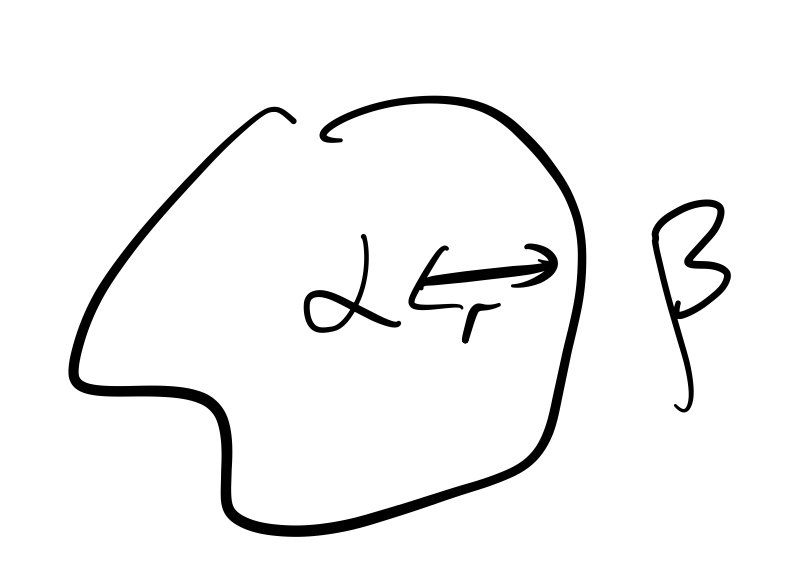
\includegraphics[scale=0.3]{Lectures/Figures/lec13-statesize.png}
\end{center}

We can define a length scale $r$ of the $\alpha$ droplet, and compute the free energy difference of the two terms:
\begin{equation}
    \Delta F = \sigma r^{d-1} - (\delta f)r^d
\end{equation}
where $\delta f$ is $F_\alpha - F_\beta$. This defines a $r_{max}$ where the free energy difference is maximized:
\begin{equation}
    r_{\text{max}} = \frac{\sigma(d-1)}{d\delta f}
\end{equation}
Looking at the maximum difference in the free energy (the barrier):
\begin{equation}
    \Delta F_{\text{max}} = \sigma\left(\frac{\sigma}{\delta f}\right)^{d-1}\left(\left(\frac{d-1}{d}\right)^{d-1} - \left(\frac{d-1}{d}\right)^{d}\right)
\end{equation}
Either $d \to \infty$ or $\delta f \to 0$ means we have large barriers between states. The latter case is find because we have two states with the same energy. $d \to \infty$ is also interesting as then the large dimension provides a big penalty/barrier.

\begin{center}
    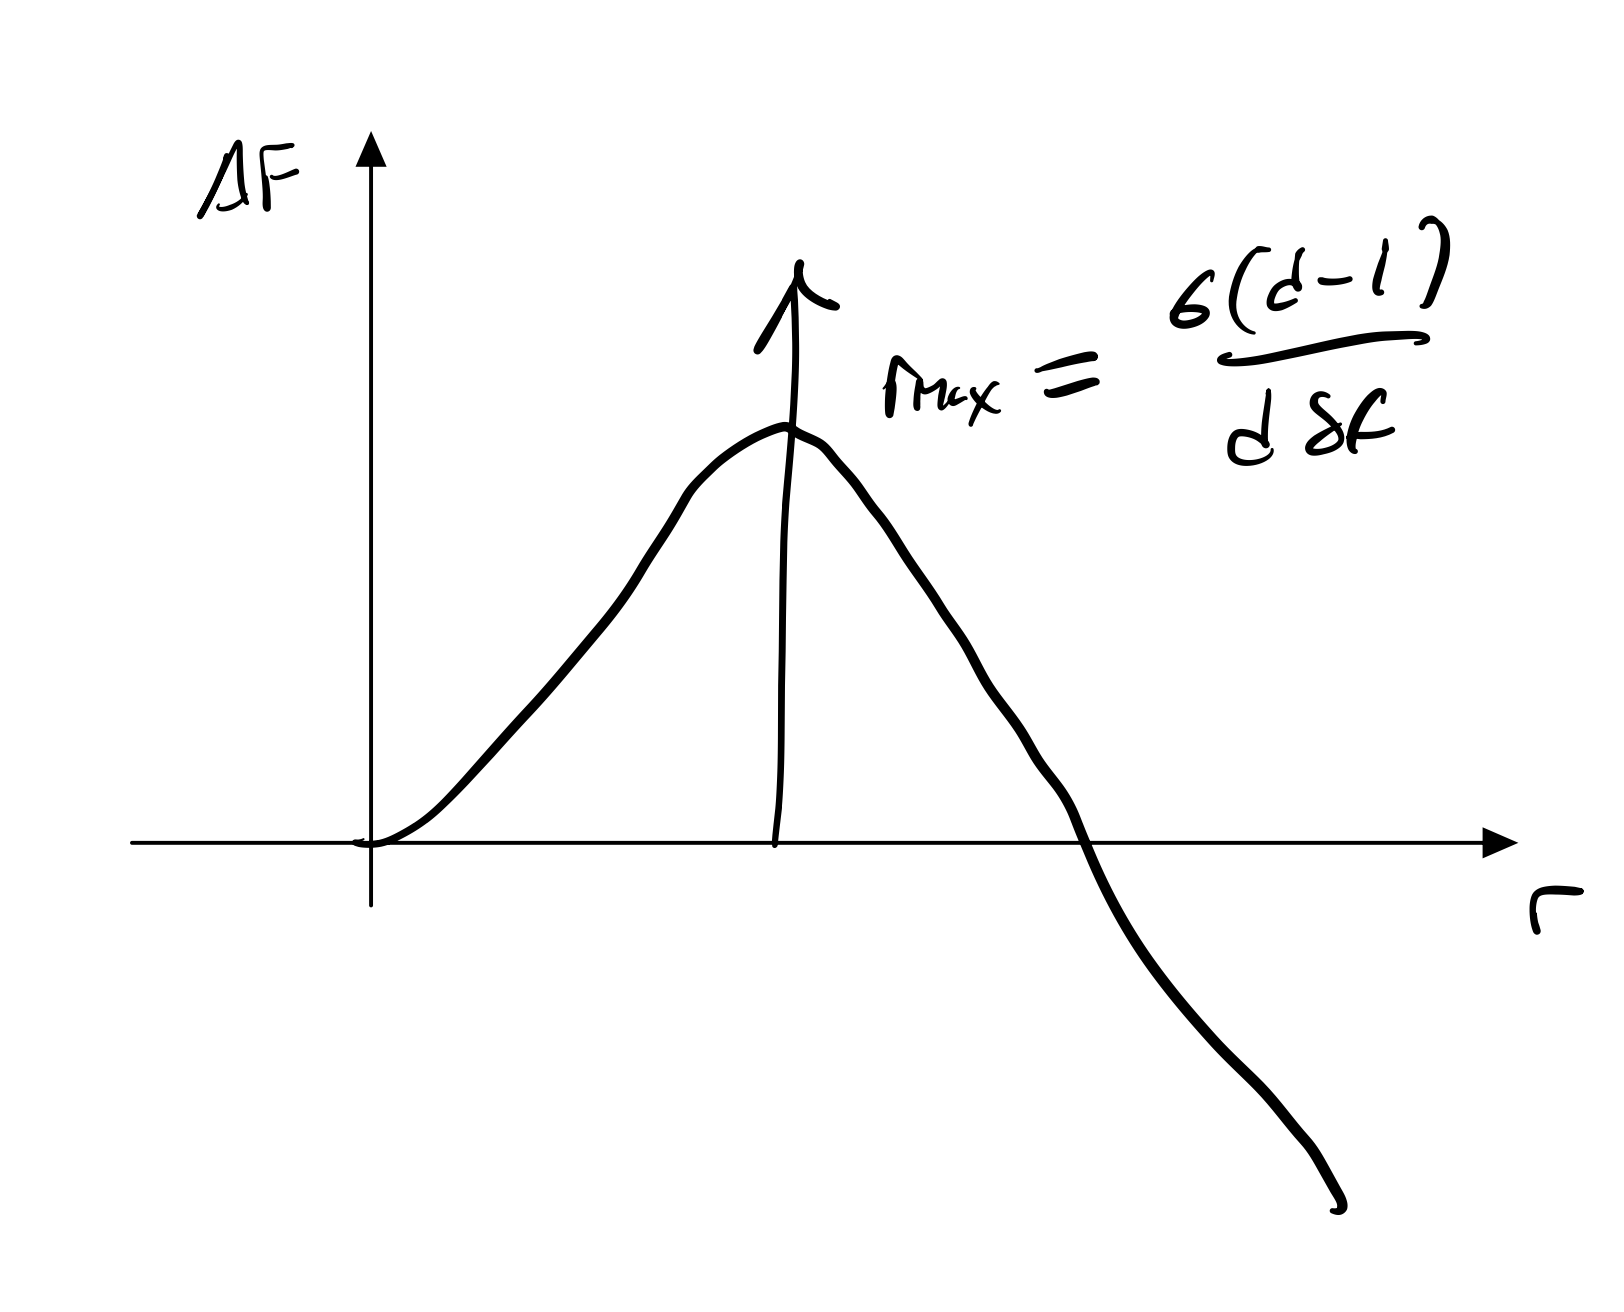
\includegraphics[scale=0.35]{Lectures/Figures/lec13-freeenergybarrier.png}
\end{center}

Next day, we look at a infinite range glass model, which is exactly solvable. At infinite temperature, despite not having any order, it has many ground states whose energies are the same, related by hierarchies.

\subsection{Order parameters}
Previously, we looked at the magnetization:
\begin{equation}
    m = \frac{1}{N}\sum_{i=1}^N \avg{\sigma_i}
\end{equation}
now we are interested in states that freeze, but do not order. This gives rise to an order parameter proposed by Edwards and Anderson, wich looks like:
\begin{equation}
    q_{EA} = \frac{1}{N}\sum_{i=1}^N \avg{\sigma_i}^2
\end{equation}
where we look at the square of the average. The spin could in principle point in any direction, which I don't care about; I care about whether the thermal average could persist forever. This is something that one in principle could atempt to measure, and would distinguish between a paramagnetic state, and a frozen but disordered state. We can generealize this to overlaps:
\begin{equation}
    q_{\sigma\tau} = \frac{1}{N}\sum_{i=1}^N \sigma_i \tau_i
\end{equation}
which taking averages:
\begin{equation}
    Q_{\alpha\beta} = \frac{1}{N}\sum_{i=1}^N \avg{\sigma_i}_{\alpha}\avg{\tau_i}_{\beta}
\end{equation}
These overlaps allow us to probe the structure in phase space. In low temperature FM, $Q_{\alpha\alpha} = 1$ while $Q_{\alpha\beta} = 0$. Conversely, for the paramagnetic states everything is zero. More concretely, $q_{++} = q_{--} = m^2$ and $q_{+-} = q_{-+} = -m^2$.
\section{Spin Glass}

\subsection{Order parameters}
Last class we introduced the Edwards-Anderson order parameter:
\begin{equation}
    Q_{EA} = \frac{1}{N}\sum_{i=1}^N\avg{\sigma_i}^2
\end{equation}
we then had the order parameter quantifying overlap:
\begin{equation}
    q_{\sigma\tau} = \frac{1}{N}\sum_{i=1}^N \sigma_i\tau_i
\end{equation}
and the average:
\begin{equation}
    Q_{\alpha\beta} = \frac{1}{N}\sum_{i=1}^N \avg{\sigma_i}_\alpha \avg{\sigma_i}_\beta
\end{equation}
where the $\avg{\cdot}_\alpha$ denotes an average over a pure state $\alpha$. 

In a glass, there is no spatial order. But, if we think about something that is frozen, if I look at a single spin and watch it for a very long time, it doesn't flip. So, order in a glass is really a statement about temporal order. The way to measure this would be to take the thermal average of a single spin $i$. If at this point I average over spins, I get zero (as there is no spatial order). But if I square it and then average, I get a finite value.

Generalizing $Q_{EA}$, we consider that our system may break ergodicity. It doesn't explore all of phase space; it gets stuck. There can be multiple states that survive for long times and are different. That said, they could potentially overlap. Thus there is an overlap matrix $Q_{\alpha\beta}$. If we take the configuration and break it up, there may be multiple pure states $\alpha, \beta$ and then there is some overlap between these states. We do the thermal average over a single site for two pure states, multiply and then take the sum.

To be more precise, when we take this thermal average, we consider:
\begin{equation}
    Q_{\alpha\beta} = \frac{1}{N}\sum_i \frac{1}{Z_\alpha}\int_{\sigma \in \alpha}\mathcal{D}\sigma \sigma_i e^{-H(\sigma)}\frac{1}{Z_\beta}\int_{\tau \in \beta} \mathcal{D}\tau \tau_i e^{-H(\tau)} = \frac{1}{Z_\alpha Z_\beta}\int_\alpha \mathcal{D}\sigma\int_{\beta}\mathcal{D}\tau q_{\sigma\tau}e^{-H(\sigma)}e^{-H(\tau)}
\end{equation}
For a paramagnet we get $Q_{\alpha\alpha} = 0$, and for a frozen state we get $Q_{\alpha\alpha}=1$. We now consider the overlap distribution:
\begin{equation}
    P(q) = \frac{1}{Z^2}\int \mathcal{D}\sigma\mathcal{D}\tau e^{-H(\sigma)-H(\tau)}\delta(q - q_{\alpha\tau})
\end{equation}
For a ferromagnet, we have two equal delta peaks when $q = \pm m^2$. 

\begin{center}
    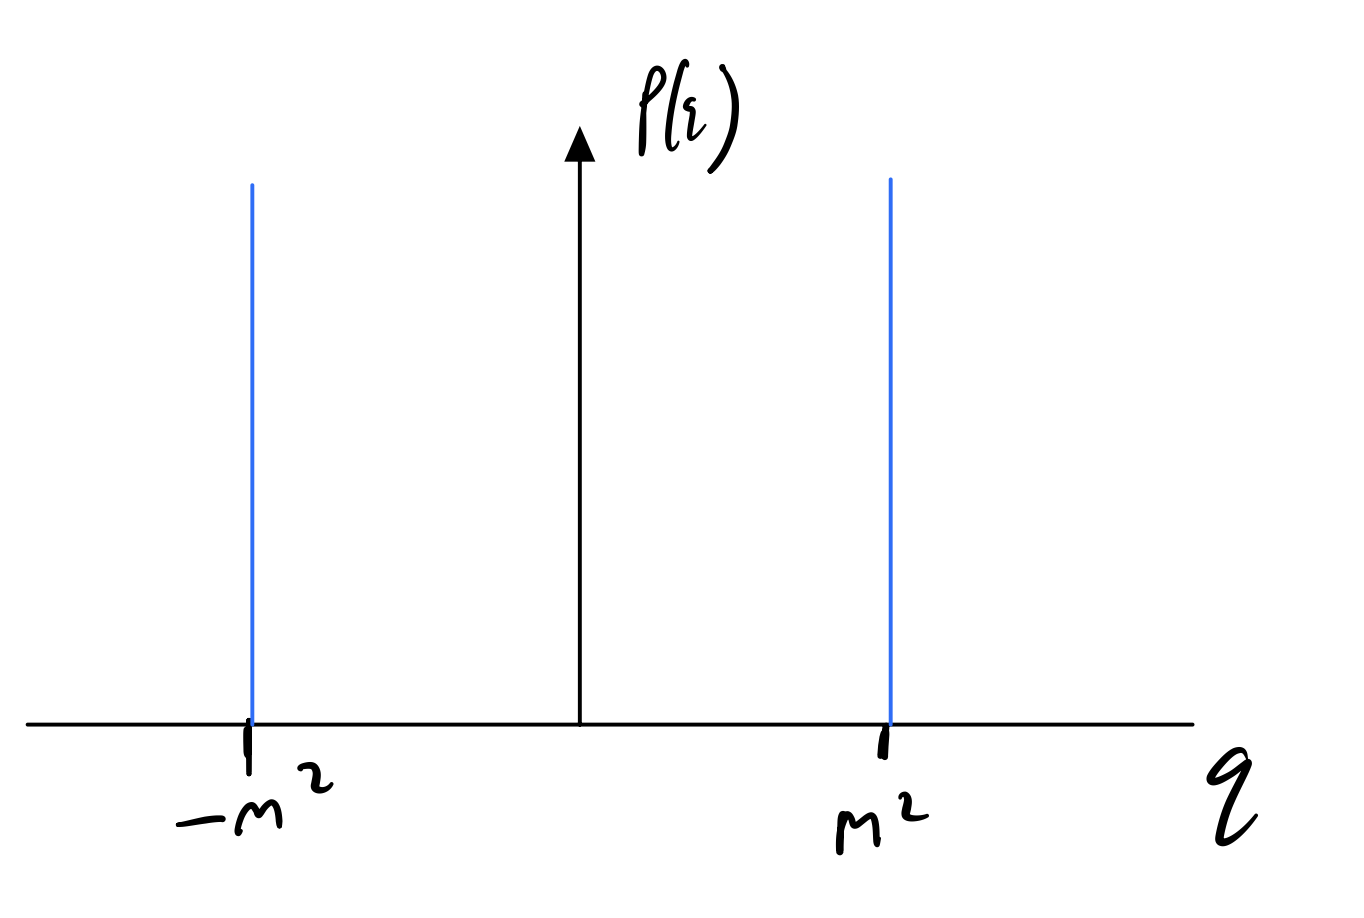
\includegraphics[scale=0.3]{Lectures/Figures/lec14-fmdist.png}
\end{center}

But note that there is generically no reason that this distribution would just be delta functions. Generically, we have delta functions + continuum part. When we find this, we have replica symmetry breaking. The two ferromagnet states have a replica symmetry, but with a continuum no such symmetry is present.

\subsection{Sherrington-Kirepatrick model}
We consider the Hamiltonian:
\begin{equation}
    H = \sum_{i,j=1}^N J_{ij}\sigma_i\sigma_j
\end{equation}
where the $J_{ij}$ are independent random variables:
\begin{equation}
    J_{ij} = \pm \frac{J}{\sqrt{N}}.
\end{equation}
This is a mostly solvable model, coming from the infinite range coupling. Note that even in a model as simple as this one, we have hidden broken symmetries and interesting phenomenology. While we are on the topic of Nobel prizes, this model was also used by Hopfield. He thought about the fact that we could use this model as a memory; if we chose $J_{ij} = \xi_i\xi_j$ with $\xi$ a vector. Then, notice that our Hamiltonian would be minimized with this choice when $\sigma = \xi$ (just a ferromagnet that's been rotated).

\subsection{$p$-spin spherical model}
The model we will actually discuss looks more complicated, but is actually easier:
\begin{equation}
    H = -\sum_{1 \leq i_2 < i_2 < \ldots < i_p \leq N} J_{i_1, \ldots, i_p}\sigma_{i_1}\sigma_{i_2}, \ldots \sigma_{i_p}
\end{equation}
where we consider $p \geq 3$. This is a $p$-spin spherical model (think about the entire set of spins as a vector), with $\frac{1}{N}\sum_{i}\sigma_i^2 = 1$. Each site $i$ has a real-valued spin. The $J$s are drawn from the Gaussian probability distribution:
\begin{equation}
    P(J) = \exp(-\frac{1}{2}J^2\frac{2N^{p-1}}{p!})
\end{equation}
where we note that $\sqrt{\bar{J}^2} \sim \frac{1}{N^{\frac{p-1}{2}}}$. Looking at the averaged $Z$ (for $p=3$):
\begin{equation}
    \overline{Z} = \int \mathcal{D}\sigma\int \prod_{i < j < k} dJ_{ijk}\exp(-\left(J_{ijk}^2\frac{N^{p-1}}{p!} + \beta J_{ijk}\sigma_i\sigma_j\sigma_k\right)) = \int \mathcal{D}\sigma\exp(\frac{\beta^2}{4N^{p-1}}p!\sum_i \sigma_i^2 \sum_j \sigma_j^2 \sum_k \sigma_k^2)
\end{equation}
Each of these sums now just gives $1$, so with the identity $p!\sum_{i>j>k} = \sum_{ijk}$, we just get the surface area of the surface:
\begin{equation}
    \overline{Z} = \exp(\frac{N\beta^2}{4})\Omega
\end{equation}
where $\Omega$ is the solid angle. Now consider $n$ replica version:
\begin{equation}
    \overline{Z^n} = \int \mathcal{D}\sigma_i^\alpha \prod_{ijk}\int dJ_{ijk}\exp(-\frac{J^2N^{p-1}}{p!} + J_{ijk}\beta\sum_{\alpha}^n \sigma_i^\alpha \sigma_j^\alpha \sigma_k^\alpha) = \int \mathcal{D}\sigma \exp(\frac{\beta^2}{4N^{p-1}}\sum_{\alpha,\beta=1}^n \left(\sum_i \sigma_i^\alpha \sigma_i^\beta\right)^p )
\end{equation}
Now we have an overlap matrix! Let us call it:
\begin{equation}
    Q_{\alpha\beta} = \frac{1}{N}\sum_i \sigma^\alpha_i \sigma^\beta_i
\end{equation}
with $Q_{\alpha\alpha} = 1$. How do we deal with this integral? We've seen this a few things, and now what we will do is to introduce an auxilary field. We introduce the trivial statement:
\begin{equation}
    1 = \int dQ_{\alpha\beta}\delta(NQ_{\alpha\beta} - \sum_i \sigma_i^\alpha \sigma_i^\beta) = \int \mathcal{D}\lambda_{ab}e^{-\lambda(NQ_{\alpha\beta} - \sigma_i^\alpha\sigma_j^\beta)}
\end{equation}
But now doing the trick:
\begin{equation}
    \delta(x) = \int dk e^{ikx}
\end{equation}
So by exponentiating the $1$, we can introduce the auxilary field $Q$:
\begin{equation}
    \overline{Z^n} = \int \mathcal{D}Q_{\alpha\beta}\mathcal{D}\lambda_{\alpha\beta}\mathcal{D}\sigma \exp(\frac{\beta^2 N}{4}\sum_{\alpha\beta}Q^p_{\alpha\beta} + N\sum_{\alpha\beta}\lambda_{\alpha\beta}Q_{\alpha\beta} - \sum_i \sum_{\alpha\beta}\sigma_i^\alpha \lambda_{\alpha\beta}\sigma_i^\beta)
\end{equation}
So then:
\begin{equation}
    \overline{Z^n} = \int \mathcal{D}Q_{\alpha\beta}\mathcal{D}\lambda_{\alpha\beta}\exp(-NS(Q, \lambda))
\end{equation}
where:
\begin{equation}
    S(Q, \lambda) = - \frac{\beta}{4}\sum_{\alpha\beta}Q_{\alpha\beta}^p - \sum_{\alpha\beta}\lambda_{\alpha\beta}Q_{\alpha\beta} - \frac{1}{2}\log\det(2\lambda_{\alpha\beta})
\end{equation}
there are no longer fluctuations of spins, but now have two fields. We have an important factor of $N$; this tells us the solution of this problem should be the saddle point of $S$, for everything away from the saddle point becomes exponentially suppressed. We need to consider the limits $n \to 0$ (we are interested in this because $F = \log Z = \lim_{n \to 0}\frac{Z^n - 1}{n}$), $N \to \infty$ (we want a large number of spins/system size, and want $N \to \infty$ so the saddle point is the solution). Then:
\begin{equation}
    -\beta F = \lim_{N \to \infty}\lim_{n \to 0}\frac{1}{nN}\int \mathcal{D}Q\mathcal{D}\lambda e^{-NS}
\end{equation}
The number of independent elements in $Q_{\alpha\beta}$ are $\frac{n(n-1)}{2}$, which as $n \to 0$ becomes negative. This is strange, but we press on - we will do this by interchanging the order of limits. We consider (to obtain the saddle point):
\begin{equation}
    \dpd{}{\lambda_{\alpha\beta}}\left[-\lambda_{\alpha\beta}Q_{\alpha\beta} + \frac{1}{2}\log \det(2\lambda)\right] = 0 \implies -Q_{\alpha\beta} + \frac{1}{2}(\lambda^{-1})_{\alpha\beta} = 0 \implies Q^{-1} = 2\lambda
\end{equation}
Thus replacing the $N \to \infty$ limit integral with the saddle point value:
\begin{equation}
    F = \lim_{n \to \infty} -\frac{1}{2\beta n}\left[\frac{\beta^2}{2}\sum_{\alpha\beta}Q^p_{\alpha\beta} + \log \det Q\right]
\end{equation}
If we now minimize w.r.t $Q$:
\begin{equation}
    0 = \dpd{F}{Q} = \frac{\beta^2 p}{2}Q_{\alpha\beta}^{p-1} + Q^{-1}_{\alpha\beta}
\end{equation}
What do we know? We know $Q_{\alpha\alpha} = 1$. Since there is nothing to distinguish the replicas (i.e. if the model is replica-symmetric) then we would say that all the off-diagonal entries of $Q$ are the same, and equal to some value $q_0$. Then, writing:
\begin{equation}
    Q_{ab} = q_0 + (1 - q_0)\delta_{ab}
\end{equation}
it is clear that:
\begin{equation}
    Q_{ab}^{-1} = \frac{1}{1-q_0}\delta_{ab} - \frac{q_0}{(1-q_0)[1 + (n-1)q_0]}
\end{equation}
here, it's a bit interesting that the $n$ shows up, and I can begin to compute this in the $n \to 0$ limit:
\begin{equation}
    \lim_{n \to 0} \dpd{F}{Q} = \frac{\beta^2 p}{2}q_0^{p-1} - \frac{q_0}{(1-q_0)^2} = 0
\end{equation}
This has two solutions. $q_0 = 0$, which is the paramagnetic, and the pair of solutions:
\begin{equation}
    q_0^{p-2}(1-q_0)^2 = \frac{2}{p\beta^2}
\end{equation}
This is a replica-symmetric solution. It has the unfortunate problem of not being stable. While it is a solution, it we look perturbatively about this solution, e.g. break the system into many pieces, we see that the energy is decreased. Another way to see the instability; it has to not just be a saddle point/extremum, but also a minimum. This requires the eigenvalues to be positive definite.

What does this mean? We still know that everything is dominated by a saddle pont, and just need to find what it is. Let's think about the average/first moment:
\begin{equation}
    q^{(1)} = \bar{Q_{\alpha\beta}}= \lim_{n\to 0} \int \mathcal{D}Q_{\alpha\beta}Q_{\alpha\beta}e^{-NS(Q_{\alpha\beta})}
\end{equation}
what happens when we average over saddle points? When we look at the $\alpha, \beta$s, we have to think about which ones we take. Eventually, this turns into:
\begin{equation}
    \bar{Q_{\alpha\beta}}= \lim_{n \to 0}\frac{2}{n(n-1)}\sum_{\alpha>\beta}Q_{\alpha\beta}
\end{equation}
This average is the first moment, and of course we can generate the $k$th moment, which gives:
\begin{equation}
    q^{(k)} = \lim_{n \to 0}\frac{2}{n(n-1)}\sum_{\alpha\beta}\overline{Q_{\alpha\beta}^k}
\end{equation}
the higher moments are more and more sensitive to the broken symmetry. We then get the distribution:
\begin{equation}
    \bar{P}(q) = \lim_{n \to 0}\frac{2}{n(n-1)}\sum_{a > b}\delta(q - Q_{ab})
\end{equation}
The distribution is governed by the fact that the likely overlap is is given by a value of $q$. Working with this probability distribution, we cab rewrite it as:
\begin{equation}
    P(q) = (1-m)\delta(q - q_1) - m\delta(q - q_0)
\end{equation}
with $0 < m < 1$. We then have the distribution:

\begin{center}
    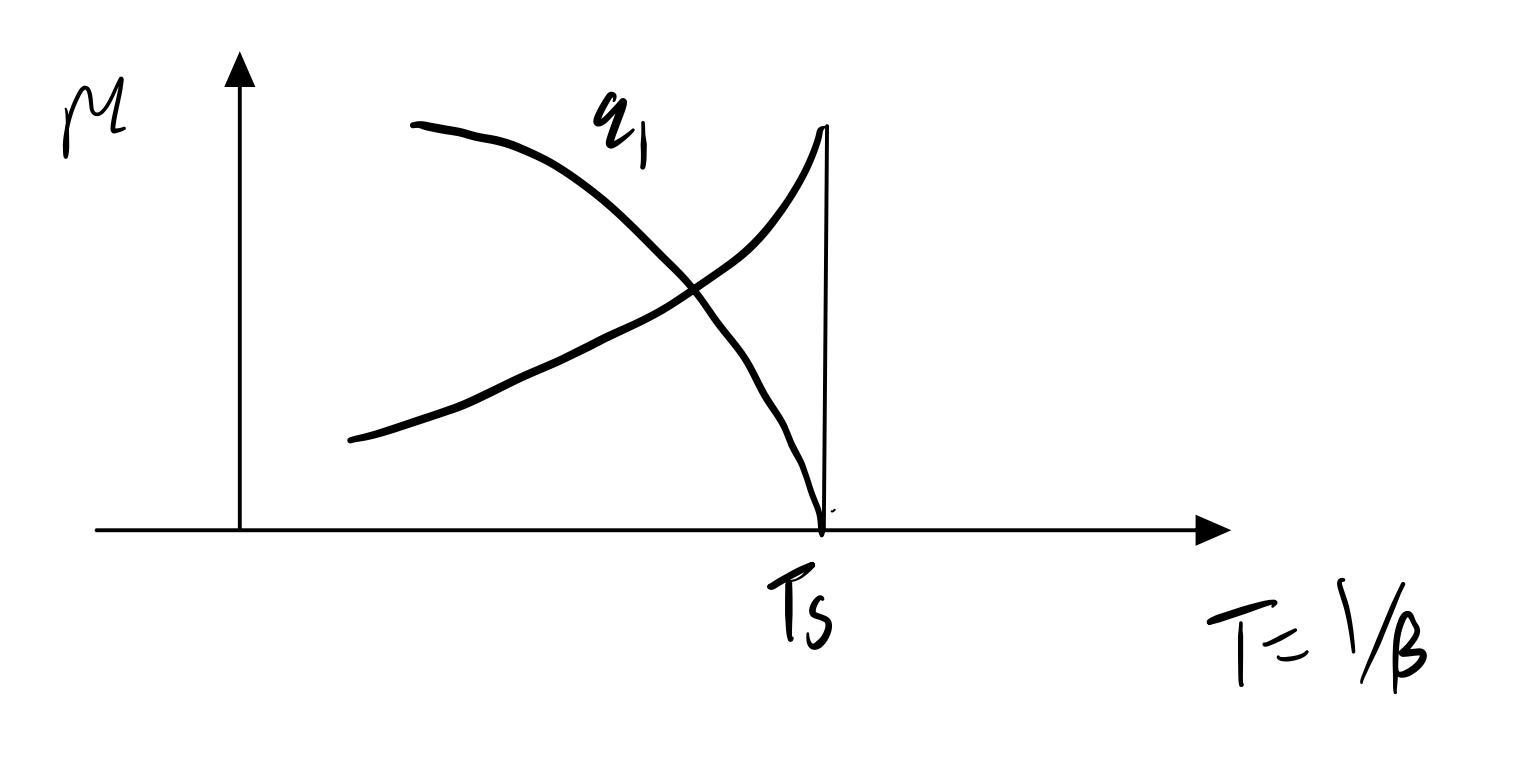
\includegraphics[scale=0.3]{Lectures/Figures/lec14-orderparam.png}
\end{center}

it is recommended to look at the homework problem before Friday - we'll come back to this last part, which we rushed a bit. What is the takehome message? The reason to writing down the odd model is that it is a mean field theory, and in MF models we are able to compute things easily from the saddle point. We are used to saddle points being very simple, but actually there is more complex structure to the saddle points than we are used to. But, if we look at finite $n$, we can visualize these solutions. We had a replica-symmetric solution, but the replica symmetry gets broken, leading to a fractal-like structure in the $Q$ matrix.
\section{Replica Symmetry Breaking, Neural Nets, Boltzmann Machines}

\emph{I was absent for this lecture, and these lecture notes are obtained from Kalpak Duddella's notes - many thanks to him!}

In this lecture, we wrap up the discussion of spin glasses and replica symmetry breaking, before moving onto the last topic of discussion for this course - Neural networks and Boltzmann machines.

\subsection{Replica Symmetry Breaking, Concluded}
We consider the replica matrix ansatz $Q_{ab}$, as you will study in HW3. Its structure ``naturally clusters'' due to off-diagonal (correlation) elements, forming a block structure about the diagonal. We obtain this by guessing the block form as the solution to the non-linear EoM and minimizing the free energy. But, we also have to check the stability of the solutions.

In more detail, we have 1s on the diagonal, $q_1$ in $m \times m$ blocks around the diagonal, and $q_0$ elsewhere, with $1 > q_1 > q_0$. We have the probability distribution:
\begin{equation}
    P(q) = \frac{m-1}{n-1}\delta(q - q_1) + \frac{n-m}{n-1}\delta(q - q_0)
\end{equation}
which as $n \to 0$ becomes the two delta peaks:
\begin{equation}
    p(q) = (1-m)\delta(q - q_1) + m\delta(q - q_0)
\end{equation}
Graphically, we have the distribution as sketched last class. In this limit, we have 1-step symmetry breaking in the exact solution of the $p$-spin spherical model.

\begin{center}
    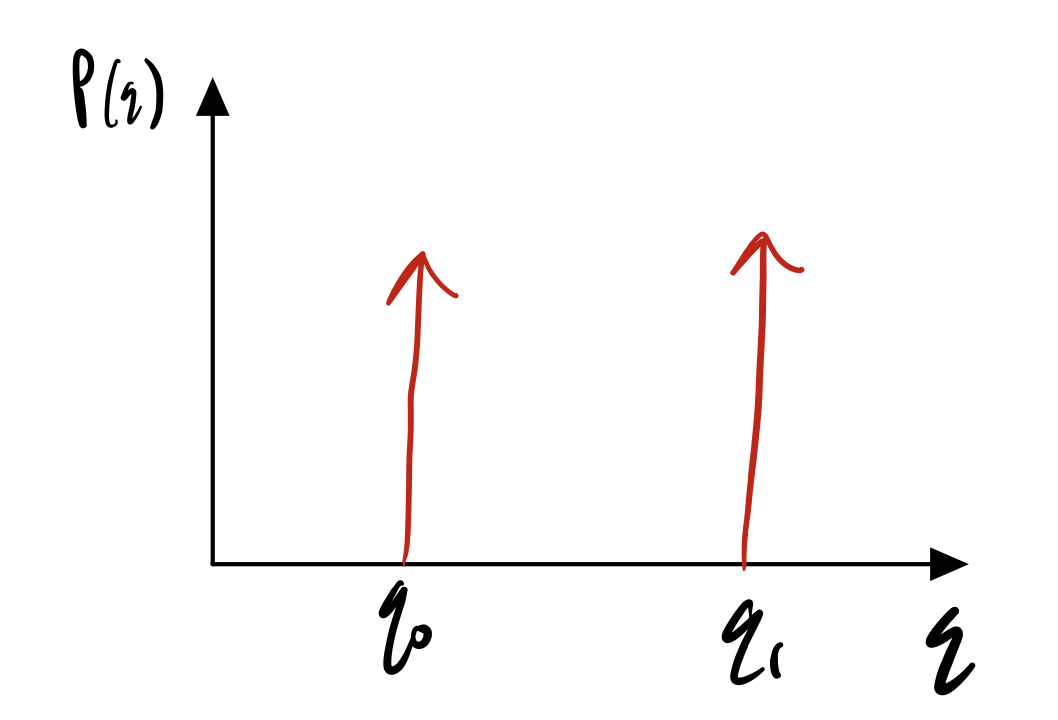
\includegraphics[scale=0.35]{Lectures/Figures/lec15-1stepsymbreak.png}
\end{center}

For $T < T_s$, we have a continuous solution where $P(a)$ varies smoothly between the two peaks at $q_0, q_1$, with peaks getting closer together as $T \to T_s$.

\begin{center}
    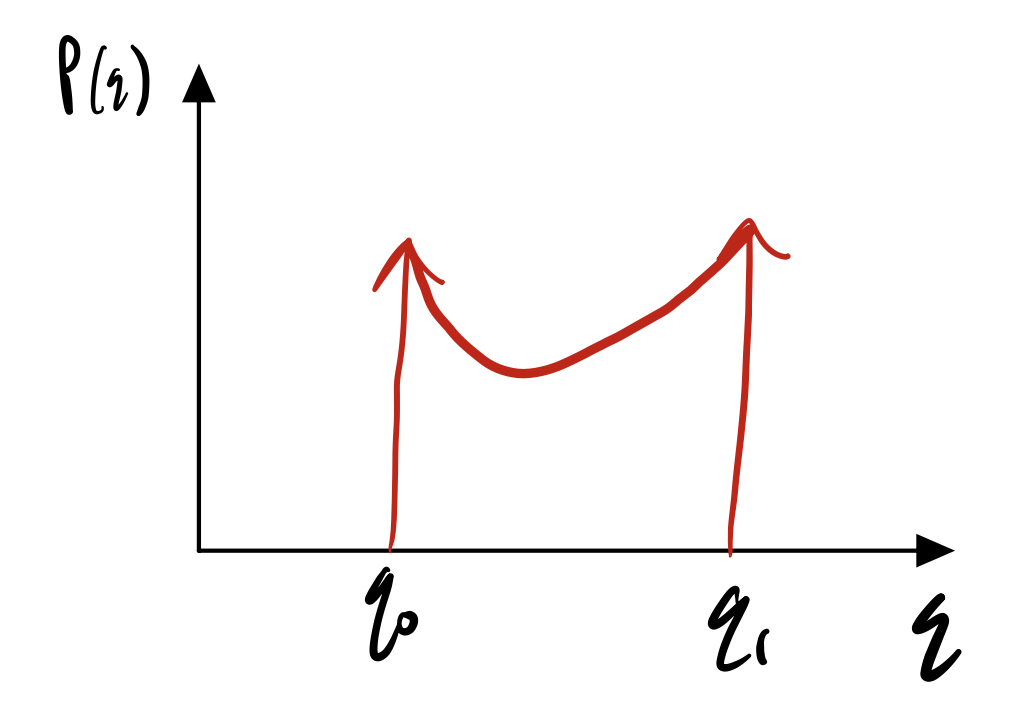
\includegraphics[scale=0.35]{Lectures/Figures/lec15-TleqTs.png}
\end{center}

For $T > T_c$, we have ``ultrametricity''; full replica symmetry breaking.

\begin{center}
    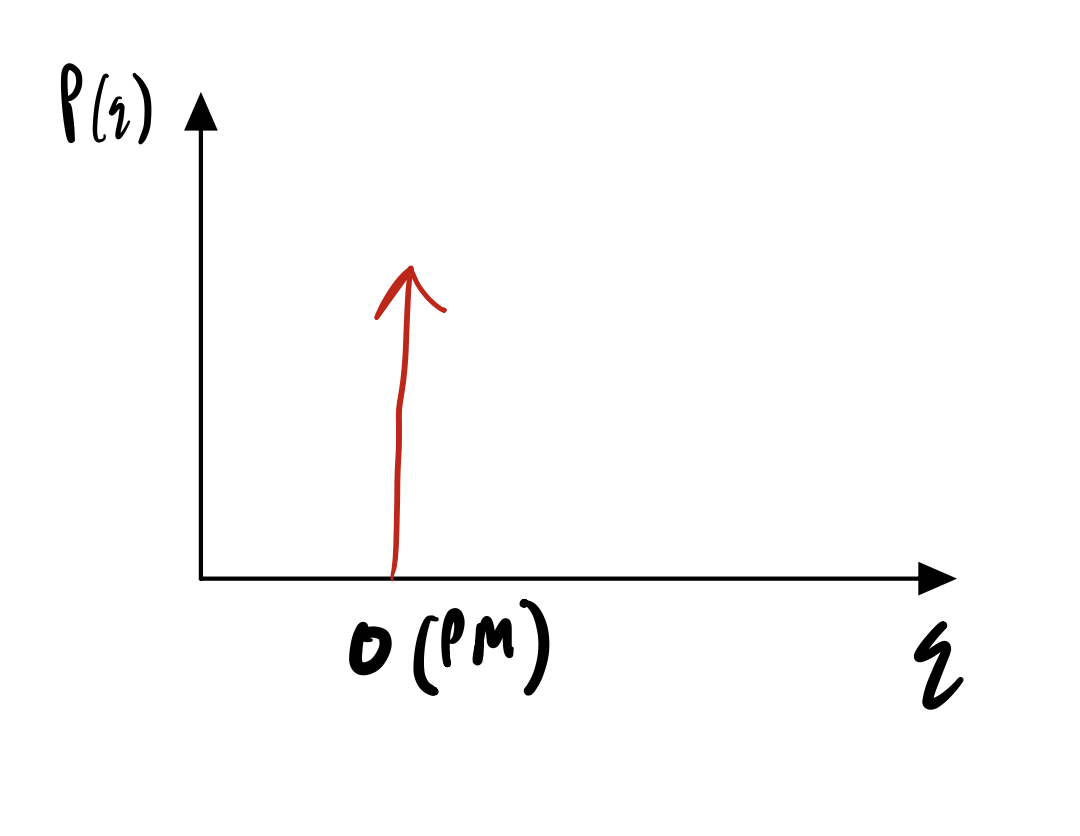
\includegraphics[scale=0.35]{Lectures/Figures/lec15-TgeqTs.png}
\end{center}

This is related to lines connecting points on the $\dpd{F}{Q}$ curve.

\begin{center}
    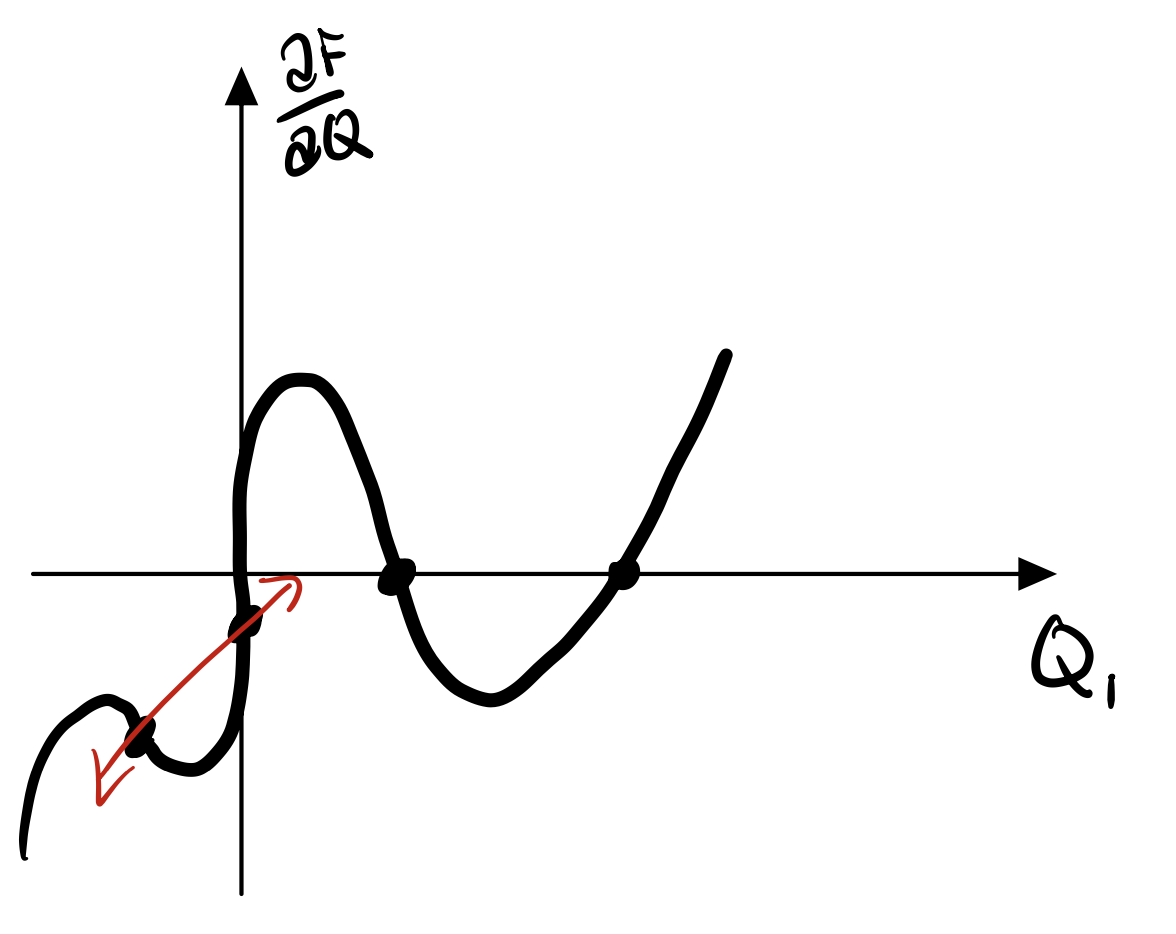
\includegraphics[scale=0.35]{Lectures/Figures/lec15-dFdQ.png}
\end{center}

\subsection{Neural Nets}
John Hopfield considered the following model for associative memory - consider the vector $\gv{\chi}$. We then store this memory by flipping spins in an (Ising) array, with system Hamiltonian:
\begin{equation}
    H = -\sum_{\avg{ij}}J_{ij}S_iS_j
\end{equation}
where the couplings are:
\begin{equation}
    J_{ij} = J\xi_i\xi_j
\end{equation}
Thus:
\begin{equation}
    H = -J\sum_i \xi_i S_i \sum_j \xi_j S_j
\end{equation}
If we now generalize to store a set of bit strings $\set{\chi^a}_a$. Then for an associative memory, we take:
\begin{equation}
    J_{ij} = \sum_a \chi_i^a \chi_j ^a
\end{equation}
with $a$ indexing over different bitstrings and $i$ indexing the position in a given bitstring. This is a ``one-layer neural network'' (we take $1 = \uparrow$, $0 = \downarrow$). Hopfield won a Nobel for a (insert choice word) ferromagnet!

For a $N \times N$ neural network, we can store about $\sim 0.15N$ memories. 

\subsection{Boltzmann Machines}
Two step phases for using Boltzmann machines:
\begin{enumerate}
    \item We first run a training phase to obtain the $\xi_i$.
    \item We then run a readout phase to allow the system to evolve on a fixed array of $J$s constructed from the learned $\xi$s.
\end{enumerate}

We consider the probability weights for a given spin configuration $s$
\begin{equation}
    P(s) = \exp(-E(s))/Z
\end{equation}
where the energy function is:
\begin{equation}
    E(s) = \sum_{ij}U_{ij}s_is_j - \sum_i b_i s_i
\end{equation}
with $U_{ij}$ the weights and $b_i$ the biases. We need to \emph{learn} the $U$s and $b$s to have the model $P(s)$ fit the data, i.e.:
\begin{equation}
    \left.P(s)\right|_{\text{model}} \approx \left.P(s)\right|_{\text{data}}.
\end{equation}

Comparing neural networks with spin models, a layered neural network corresponds to an auxiliary field model.

\begin{center}
    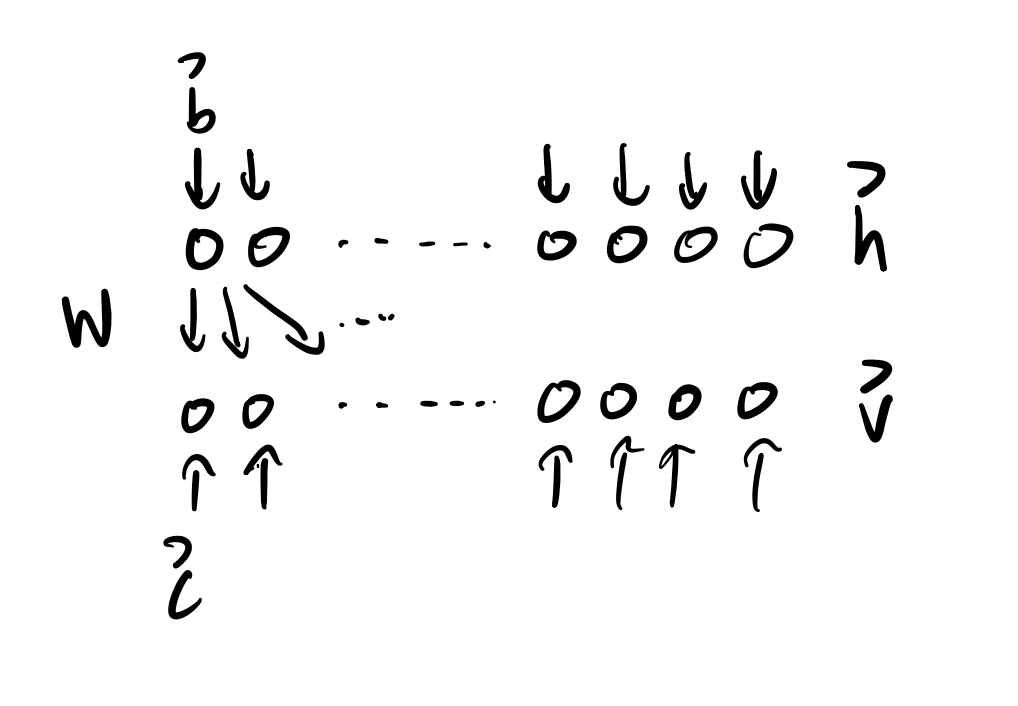
\includegraphics[scale=0.35]{Lectures/Figures/lec15-NN.png}
\end{center}

For simplicity, we consider a 2-layer network, composed of a hidden layer of nodes (vector of spins) $\v{h}$ and a visible layers of nodes $\v{v}$. We have a bias $\v{b}$ on the hidden nodes and $\v{c}$ on the visible nodes. We also have a weight-matrix $W$ between the two layers which computes ``scores'' as a linear transformation.

The energy of a neuron configuration specified by $\v{v}, \v{h}$ is:
\begin{equation}
    E(v, h) = -\v{b} \cdot \v{v} - \v{c} \cdot \v{h} - v_iW_{ij}jh_j
\end{equation}
We then have the conditional probabilities:
\begin{equation}
    P(\v{h} \vert \v{v}) = \prod_i P(h_i \vert \v{v})
\end{equation}
\begin{equation}
    P(\v{v} \vert \v{h}) = \prod_i P(v_i \vert \v{h})
\end{equation}
Which we can also write as:
\begin{equation}
    P(\v{h} \vert \v{v}) = \frac{P(\v{h}, \v{v})}{P(\v{v})} = \frac{1}{P(\v{v})Z}e^{\v{b} \cdot \v{v} + \v{c} \cdot \v{h} + v_iW_{ij}h_j} = \frac{1}{Z'}e^{\v{c} \cdot \v{h} + v_iW_{ij}h_j}
\end{equation}
With $\frac{1}{Z'} = \frac{1}{P(v)Z}e^{\v{b} \cdot \v{v}}$. 

Now, we have some data probability ditribution $P_{\text{data}}(\v{x})$. We have a model probability distribution $P_{\text{model}}(\v{x};\gv{\theta})$ with model parameters $\gv{\theta}$. The goal is to find the optimal model parameters, obtained from:
\begin{equation}
    \gv{\theta}_{\text{model}} = \text{argmax}_{\theta}\prod_{i=1}^m P_{\text{model}}(x_i, \theta) = \sum_{i=1}^m \log P_{\text{model}}(x_i, \theta)
\end{equation}
\section{Non-equilibrium Dynamics}
Today we will discuss the Fokker-Planck equation and how to derive Field theories. We won't have time to discuss anomalous diffusion; how to start with a differential equation that looks like it should scale in an obvious way and then get interesting critical exponents. There's also interesting discussion of analyzing a laser through a statistical field theory lens, which we will not quite get to.

\subsection{Diffusion Equation ($V = 0$)}
Our basic starting point is an equation of motion of the form:
\begin{equation}
    m\ddot{x} = -\frac{\dot{x}}{\mu} - \dpd{V}{x} + f_{\text{noise}}(t)
\end{equation}
i.e. a particle moving deterministically in a potential under the influence of drag and stochastic noise. The potential term leads to ballistic motion, while the noise term leads to diffusive motion. We consider the limit of small $\ddot{x}$ where we can neglect the acceleration term, thus:
\begin{equation}
    \dot{x} = v(x) + \eta(t)
\end{equation}
with:
\begin{equation}
    v(x) = -\mu\dpd{V}{x}
\end{equation}
and:
\begin{equation}
    \avg{\eta} = 0
\end{equation}
\begin{equation}
    \avg{\eta(t)\eta(t')} = 2D\delta(t-t')
\end{equation}
i.e. Markovian white noise.

In the $V = 0$ case, we have the solution:
\begin{equation}
    x(t) = x(0) + \int_0^t dt'\eta(t')
\end{equation}
where:
\begin{equation}
    \avg{(x(t) - x(0))^2} = \int_0^t d\tau_1 \int_0^t d\tau_2 \avg{\eta(\tau_1)\eta(\tau_2)} = 2Dt.
\end{equation}
We then obtain the propagator of the diffusion equation:
\begin{equation}
    P(x, t) = G(x, t, 0, 0) = \frac{1}{(4\pi D t)^{3/2}}e^{-\frac{x^2}{4D}t}
\end{equation}
With $P$ the solution of:
\begin{equation}
    \dpd{P}{t} = -D\nabla^2 P
\end{equation}
this is the familiar diffusion equation.

\subsection{Fokker-Planck Equation ($V \neq 0$)}

Let's now look at advancing time by some small time $\e$:
\begin{equation}
    P(x, t + \e) = \int d^3x' P(x', t)\bra{x}T_\e\ket{x'}
\end{equation}
where $\bra{x}T_\e\ket{x'}$ represents a transition amplitude.

Splitting up the two parts of the motion:
\begin{equation}
    x = x' + v(x)\e + \eta_\e
\end{equation}
where:
\begin{equation}
    \eta_\e = \int_t^{t+\e}dt\eta(t)
\end{equation}
which has the properties:
\begin{equation}
    \avg{\eta_\e} = 0
\end{equation}
\begin{equation}
    \avg{\eta_\e^2} = 6D\e.
\end{equation}
With this, we can define the transition matrix amplitude:
\begin{equation}
    \bra{x}T_\e\ket{x'} = \frac{1}{(4\pi D\e)^{3/2}} \exp(\frac{-(x - x' - \e v(x'))^2}{4D\e})
\end{equation}
Let us explain this. If we had a potential, the particle would have rolled to a specific place deterministically from $x'$. If the particle instead reaches $x$, we need the noise to be precisely the correct magnitude for the particle to get to the position we want it to be, which gives us the above expression. Then:
\begin{equation}
    P(x, t) = \int d^3x' \frac{1}{(4\pi D\e)^{3/2}}P(x', t) \exp(\frac{-(x - x' - \e v(x'))^2}{4D\e})
\end{equation}
for $\abs{x - x'}$ small we can then replace $P(x', t)$ in the integral with $P(x, t)$, and linearize:
\begin{equation}
    \dpd{P}{t} + \nabla \cdot \v{J} = 0 \implies \v{J} = \v{v}P - D\nabla P
\end{equation}
The interpretation of this is intuitive. We have a drift current (from the potential) and a diffusion current (from the noise).

The stationary/equilibrium station is:
\begin{equation}
    P_{\text{eq}}(x) = e^{-V(x)/k_B T}
\end{equation}
with:
\begin{equation}
    \nabla P_{\text{eq}} = \frac{\v{v}}{\mu k_B T}P_{\text{eq}} \implies D = \mu k_B T
\end{equation}
So we identify what the parameter $D$ must be. This is usually called the ``fluctuation-dissipation'' theorem.

\subsection{Generalizing to a field - Model A}
We write down the Hamiltonian as a function of a field $m$:
\begin{equation}
    H[m] = \int d^dx \left(\frac{1}{2}rm^2 + \frac{1}{4}um^4 + \frac{1}{2}\kappa (\nabla m)^2 + \ldots \right)
\end{equation}
The analogous EoM is:
\begin{equation}
    \dpd{m}{t} = -\mu\frac{\delta H}{\delta m} + \eta(t) = -\mu r m - \mu u m^3 + \mu \kappa(\nabla^2 m) + \eta
\end{equation}

In the Gaussian theory (taking $u = 0$) we have:
\begin{equation}
    \dpd{m(q, t)}{t} = -\mu(r + \kappa q^2)m + \eta
\end{equation}
where:
\begin{equation}
    \avg{\eta} = 0
\end{equation}
\begin{equation}
    \avg{\eta_q\eta_{q'}} = 2D\delta(t-t')\delta(q-q')(2\pi)^d
\end{equation}
There is then a $q$-mode decay time:
\begin{equation}
    \frac{1}{\tau(q)} = \mu(r + \kappa q^2)
\end{equation}
from this we can determine what happens to the fluctuations:
\begin{equation}
    \avg{m(q, t)m(q', t)} = \frac{D\delta(q + q')}{\mu(v + \kappa q^2)}
\end{equation}
where there is no time-dependence for we have performed an ensemble average. At very long times the distribution approaches the Lorentzian. Note that $\frac{D}{\mu} = k_B T$. This is what is known as ``critical slowing down''.

In some sense we pulled the EoM out of a hat, and its not the most general EoM we could have written down. In particular we notice the order parameter is not conserved. This specific model is known as model A. There are models A-F, check out the review article by Honenberg in reviews of modern physics if interested. But for now, we only study A/B.

\subsection{Model B}
Now consider a model where we do want the order parameter to be conserved:
\begin{equation}
    \dod{}{t}\int d^dx m(x, t) = 0
\end{equation}
so we now have the equation of motion:
\begin{equation}
    \dpd{m}{t} = -\nabla j + \nabla \sigma
\end{equation}
with $j = \mu v$ and $\sigma \sim \eta$. This new model has the constraint that the magnetization is fixed, and this gets rid of low-order derivatives. We thus end up with:
\begin{equation}
    \dpd{m}{t} = \mu v \nabla^2 m - \mu \kappa \nabla^4 m + \eta
\end{equation}
Thus we have different dynamics associated with the conservation of the order parameter.

\subsection{Noise and Optimal Trajectories}
The above was all pretty heuristic. Let's explore something that's less heuristic, with a similar starting point:
\begin{equation}
    \dot{X} = A(X) + B\xi
\end{equation}
with $\avg{\xi\xi} = 2D\delta(t - t')$. 

We solve this via the identity:
\begin{equation}
    1 = Z[\xi] = \int \mathcal{D}X(t)\;J(X)\delta[\p_t X - A(X) - B\xi]
\end{equation}
where we have stuck in the EoM as a delta function.

We then generate an auxilary field $X^q$ using an identity:
\begin{equation}
    Z[\xi] = \int \mathcal{D}X(t)\int \mathcal{D}X^q(t)\exp(-2i\int dt X^q(t)(\p_t X - A - B\xi))
\end{equation}
Why we set this up is so that we can integrate over the noise (also let's set $B = 1$):
\begin{equation}
    Z = \int \mathcal{D}\xi e^{-\frac{1}{4}\int dt \xi^2}Z[\xi] = \int \mathcal{D}X\mathcal{D}X^q \exp(\int dt \left[-2iX^q(\p_t X - A(X)) - 4(X^q)^2\right])
\end{equation}
We now have an action that is a function of two fields. Faced with something like this, we look at the saddle point equations (here of two variables). This yields two equations:
\begin{equation}
    \dot{X} = A(X) + 4iX^qD(X)
\end{equation}
\begin{equation}
    i\dot{X}^q = -iX^qA'(X) + 2(X^q)^2D'
\end{equation}
with $' = \dpd{}{X}$. $X^q$ must be imaginary since $X$ is real. Let us do a change of variables $P = 2iX^q$. In this case, it turns out that we can write the equations of motion we saw above as:
\begin{equation}
    \dot{X} = \p_P H[P, X]
\end{equation}
\begin{equation}
    \dot{P} = -\p_X H[P, X]
\end{equation}
with:
\begin{equation}
    H = PA(X) + P^2 D(X).
\end{equation}
These look exactly like Hamilton's equations! $X^q$ ``looks like'' a conjugate momentum. We can then identify an action:
\begin{equation}
    iS[X, P] = - \int dt [P\dot{X} - H]
\end{equation}
and think about optimal trajectories. The simplest one to think about would be to take $A(X) = -\dpd{V}{X}$, Since $D(X) \sim T$, we have two stable trajectories where $H$ is zero; when $P = 0$, or when $P = -\frac{A}{D}$. Sketching the flows in phase space:

\begin{center}
    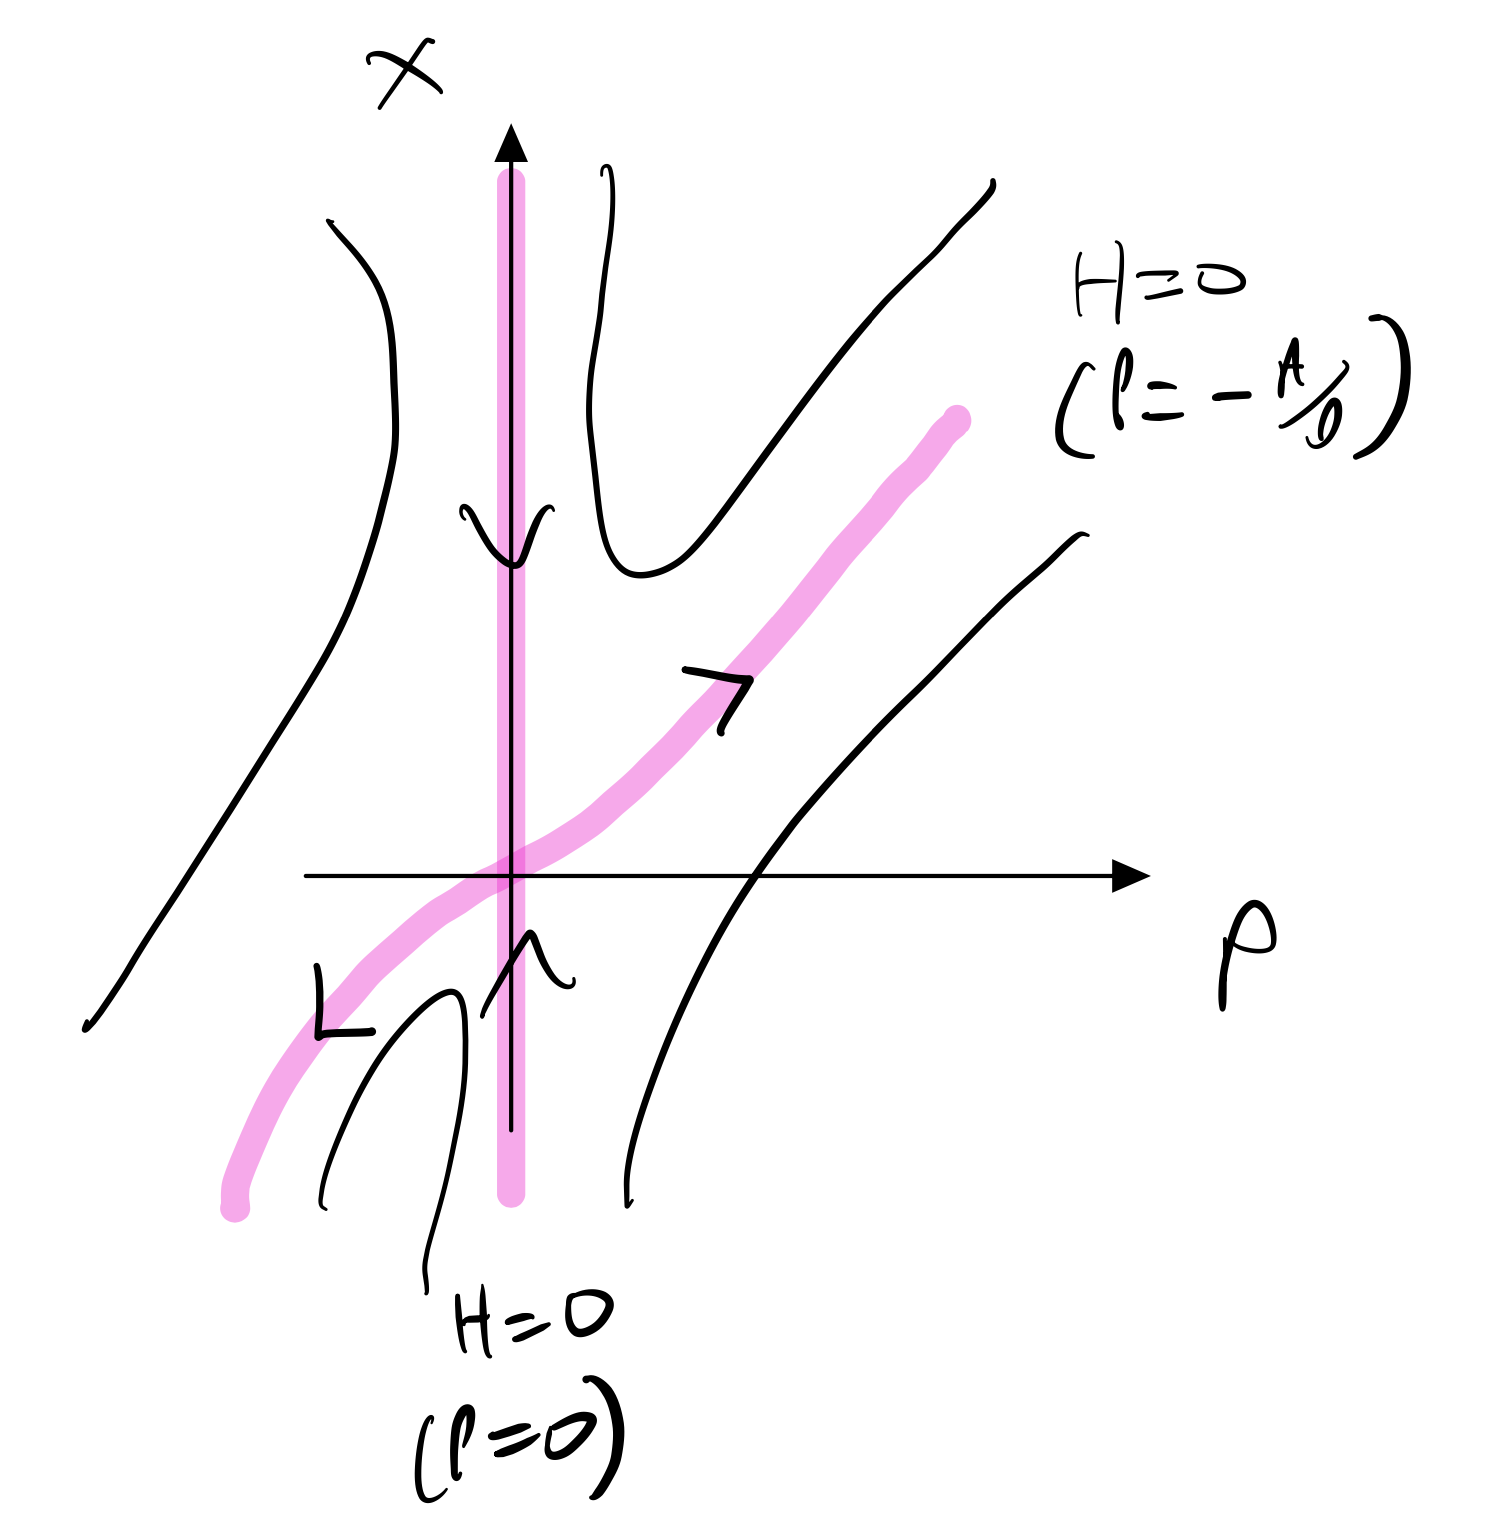
\includegraphics[scale=0.3]{Lectures/Figures/lec16-phasespace.png}
\end{center}

In equilibrium of this problem, what is $P(X_0)$? Let us write the action:
\begin{equation}
    iS[X_0] = - \int dt P\dot{X} = -\int_0^{X_0}P(X)
\end{equation}
Then taking $P(X) = -\frac{A}{D} = -\frac{V'}{D}$:
\begin{equation}
    iS[X_0] = -\frac{1}{T}\int_0^{X_0}dx V'(X) = \frac{1}{T}(V - V_0)
\end{equation}
which is just the Boltzmann distribution!

A last point. Suppose the potential has a metastable minimum:

\begin{center}
    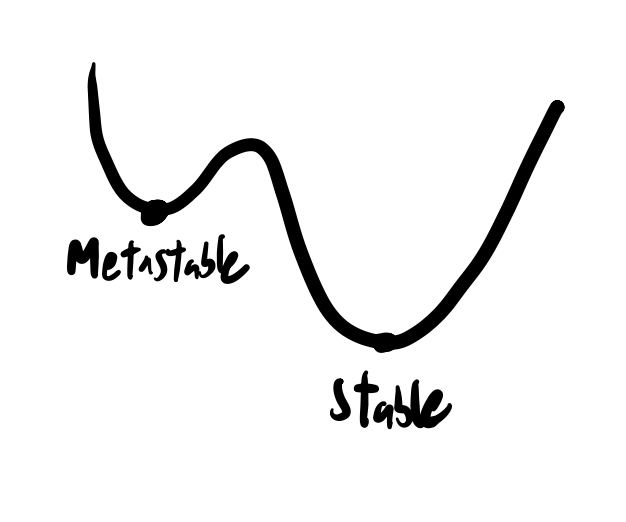
\includegraphics[scale=0.4]{Lectures/Figures/lec16-metastableminima.png}
\end{center}

Then, what I am interested in is the probability of escape, given by the shaded region:

\begin{center}
    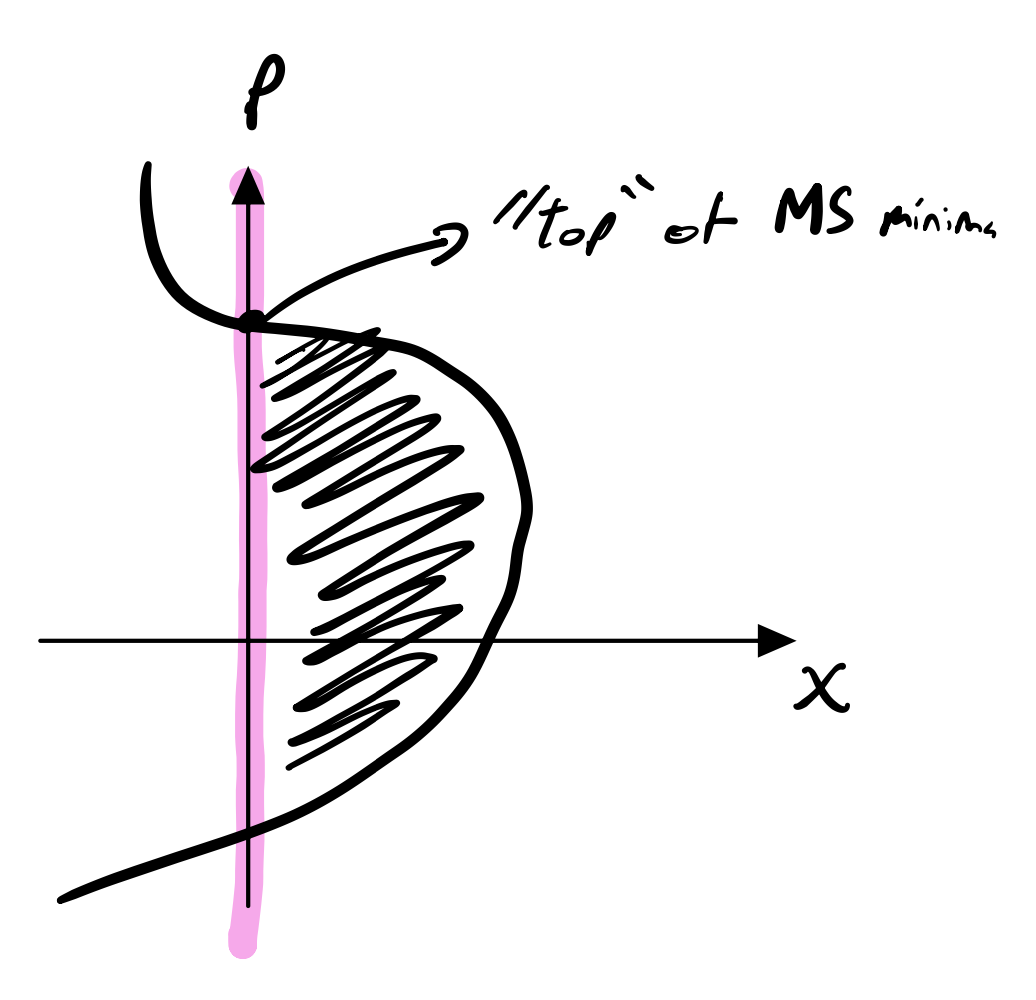
\includegraphics[scale=0.3]{Lectures/Figures/lec16-metastablephase.png}
\end{center}

which gives:
\begin{equation}
    S[X_S] = -\frac{V(X_S) - V(0)}{T}
\end{equation}
which is just WKB.

Here, we find an optimal trajectory, which gives us where we want to be. This is of course an approximation. We can go back and add more terms to our theory, making it a dynamical field theory. 

Note: The best review of this material comes from Kamenev.

\subsection{Where have we come?}
There are generic and universal properties of theories. They are made most evident at the point where these theories are hardest to solve. The underlying principle behind this universality is scaling and embodied by the renormalization group. The definition of the interesting point/phase transition is associated with the scale invariant quantities. This doesn't always happen, and almost any real system deviates from this, but such deviation can itself lead to interesting phenomenology, e.g. in the case of disorder and spin glasses.

If you have the time, next week we'll discuss quantum critical points (adding back the non-linear terms and seeing their effects). We will also study the laser and fluids/porous media, which gives us anomalous scaling/stretched power laws. 

\end{document}